\documentclass[editMode]{00_ufdissertation}\sloppy
\usepackage[colorlinks=true]{hyperref}
%%%%%%%%%%%%%%%%%%%%%%%%%%%%%%%%%%%%%%%%%%%%%%%%%%%%%%%%%%%%%%%%%%%%%%%%%%%%%%%%
%%%                 User Package and Style File loading.
%%%%%%%%%%%%%%%%%%%%%%%%%%%%%%%%%%%%%%%%%%%%%%%%%%%%%%%%%%%%%%%%%%%%%%%%%%%%%%%%

%\usepackage{CustomMacros}%  This is a user macro/style file.

\usepackage{tikz}%       tikz is used by almost everyone, but certainly by me for this.
\usepackage{pgfplots}%   pgfplots is tikz but better.

\usepackage{algpseudocode}

\usepackage{booktabs} %This package can be used to make heavier/lighter \hline commands with \toprule, \midrule, \bottomrule
\usepackage{tabularray}
\usepackage{graphicx}


\usepackage{scrextend}
\deffootnote{1.5em}{0em}{\thefootnotemark\quad}
\usepackage[all]{nowidow} %avoids single lines of text at the top or bottom of page.  If any of your packages cause this package not to work, you will have to manually remove any orphans/widows or add a line penalty
%%%%%%%%%%%%%%%%%%%%%%%%%%%%%%%%%%%%%%%%%%%%%%%%%%%%%%%%%%%%%%%%%%%%%%%%%%%%%%%%
%%%                     User Configuration commands
%%%%%%%%%%%%%%%%%%%%%%%%%%%%%%%%%%%%%%%%%%%%%%%%%%%%%%%%%%%%%%%%%%%%%%%%%%%%%%%%

%% Uncomment the relevant line below if you have tables or figures.
\haveTablestrue%        Uncomment this if you have tables in your thesis.
\haveFigurestrue%       Uncomment this if you have figures in your thesis.
%\haveObjectstrue%       Uncomment this if you have Objects in your thesis. This is almost certainly not the case however.

%%%%%%%%%%%%%%%%%%%%%%%%%%%%%%%%%%%%%%%%%%%%%%%%%%%%%%%%%%%%%%%%%%%%%%%%%%%%%%%%
%%% Below are the commands to set the degree type, department, graduation time, and chair. 
%       Most of these are self explanatory. 
%       Note: The \chair command takes an optional argument for a cochair. 
%           So if John was your chair and Jacob was a cochair, you would use \chair[Jacob]{John}.
%           If John was your chair and you had no cochair, you can simply use \chair{John}.
%%%%%%%%%%%%%%%%%%%%%%%%%%%%%%%%%%%%%%%%%%%%%%%%%%%%%%%%%%%%%%%%%%%%%%%%%%%%%%%%

\title{The working title of Nicholas Terrel's doctoral dissertation}%  Put your title here.

\degreeType{Doctor of Philosophy}%   Official name of your degree; eg "Doctor of Philosophy".
\major{Chemistry}%                    Your official Department
\author{Nicholas Terrel}%                  Your Name
\thesisType{Dissertation}%              Dissertation (PhD) or Thesis (Masters)
\degreeYear{2025}%                      Intended graduation year (not the year you submit the thesis)
\degreeMonth{May}%                   Month of graduation should be May, August, or December.
\chair{Adrian Roitberg}%                   Chair and Cochair (see comment block above).

%%%%%%%%%%%%%%%%%%%%%%%%%%%%%%%%%%%%%%%%%%%%%%%%%%%%%%%%%%%%%%%%%%%%%%%%%%%%%%%%
%%% For each of the following, type in the name of the file that contains each section. 
% They are assumed to be tex files, but if they aren't the command takes an optional argument for the extension.
%So, you could load dedication.tex as your dedication file using \setDedicationFile{dedication}
% You could load dedication.txt instead with \setDedicationFile[txt]{dedication}.

% NOTE: For some compilers they may or may not add a .tex to the end of the file automatically.
% If you get a "couldn't find dedication.tex.tex" type error, try the command with an empty optional argument,
%e.g. \setDedicationFile[]{dedication}
%%%
%%%%%%%%%%%%%%%%%%%%%%%%%%%%%%%%%%%%%%%%%%%%%%%%%%%%%%%%%%%%%%%%%%%%%%%%%%%%%%%%

%%% These are REQUIRED sections; easiest to do via these commands.

\setDedicationFile{01_dedication}%                 Dedication Page
\setAcknowledgementsFile{01_acknowledgements}%     Acknowledgements Page
\setAbstractFile{01_abstract}%                     Abstract Page (This should only include the abstract itself)
\setReferenceFile{8_references}{achemso}%         References. First argument is your bibtex source file
%                                                       the second argument is your bibtex style file.

\setBiographicalFile{9_biography}%                Biography file of the Author (you).

%%% These are NOT required, so only use them if you actually need/have them.

\setAbbreviationsFile{01_abbreviations}%           Abbreviations Page
\setAppendixFile{7_appendix}%                     Appendix Content; hyperlinking might be weird.
\multipleAppendixtrue%                          Uncomment this if you have more than one appendix, 
%                                                   comment it if you have only one appendix.


%%%%%%%                     End of File Assignment
%%%%%%%%%%%%%%%%%%%%%%%%%%%%%%%%%%%%%%%%%%%%%%%%%%%%%%%%%%%%%%%%%%%%%%%%%%%%%%%%

\begin{document}

%%%% Here you just need to include/input your actual work. 
%       The above files (dedication, acknowledgement, titlepage, etc etc) will all be added for you 
%       using the files you assigned above. 
%       If you want to input the above files manually you can comment out the \setFILE command above 
%       and use \input or \include here. Generally you want to use \include to get your pagebreak.
%       NOTE: If you input manually you will have to do some/all the formatting manually.

\bibstyle{achemso}% Removed \usepackage{} command from line 11 and set the bibliography style here instead (must be within \begin{document})

\chapter{Introduction and background} 
\label{top_of_intro}
The landscape of computational chemistry has shifted greatly over the past decade. 
The development of computational tools for chemical physics centers on approximating solutions to the Schr{\"o}dinger equation \cite{schrodinger_eqn}, whether through the development of electronic structure theory or, more indirectly, by employing classical mechanics to model molecular dynamics (MD) with force fields that have been tuned to experimental and high-accuracy quantum mechanical (QM) data.
Prior to the emergence of machine-learned methods, advancements in the field were driven by specialized approaches to solving chemical equations \cite{trp_cage_roitberg, dft_qm_mm_roitberg}, 
as well as relying on the exponential growth of hardware capabilities to simulate increasingly complex systems.
Well-established \textit{ab initio} quantum chemical methods, such as density functional theory (DFT) \cite{dft_first_paper, perspective_fifty_years_DFT, wB97X}
or coupled cluster methods \cite{coupled_cluster_first_paper, ccsd(t)_f12, dplno_ccsd(t)*},
provide close agreement with experimental methods and have long been considered the gold standard for electronic structure calculations.
Such methods carry a computational cost that scales steeply with system size---at $O(N^3)$ or greater scaling with $N$ electrons---limiting their utility in simulation of large systems or timescales relevant to many macroscopic observations. 

Computational chemistry has the persistent challenge of balancing chemical accuracy and computational cost. 
With few exceptions, approximations are necessary to determine a solution for any chemical system of interest. 
There are a variety of options for computing molecular energies but, regardless of the sophistication of the approach taken in approximating a potential energy surface (PES), there is a trade-off between the level of detail of the system and the chemical accuracy of the determined solution.
Efficient sampling techniques \cite{remd_adrian1, remd_adrian2, remd_umbrella} 
and hardware acceleration \cite{gpu_dft, gpu_quantum_chem1, gpu_quantum_chem2} 
played an essential role in mitigating some of these computational bottlenecks during the early 21st century.
The 2010s saw great strides in parallel computing, namely incorporating graphics processing units (GPUs) in chemical simulations \cite{ gpu_accelerated_AMBER, gpu_accelerated_AMBER18}
and \textit{ab initio} computations \cite{parallel_ab_initio_luehr}. 
The  complexity of larger systems make full QM calculations computationally prohibitive, necessitating hybrid approaches such as QM/MM to balance accuracy and efficiency in order to model the behavior of, for example, protein-ligand interactions \cite{dft_qm_mm_roitberg, QMtoMM_thermo_cycle}.
Some approaches to \textit{ab initio} computations increase computational efficiency by using lower-level theory with corrections to correlate with higher-accuracy methods, such as atom-centered potentials applied in the Hartree-Fock method \cite{correcting_HF_atom_centered_potentials}, though such approaches rely on hand-tuning which limits their utility as generalized potential models.
The need for a paradigm shift was clear: in order to address chemical problems ever-growing in complexity, new methodologies for efficiently computing results at quantum-levels of accuracy needed to be explored.
The work detailed here exists at this intersection, with the aim of bridging the gap between the chemical accuracy of interatomic potential models and the computational efficiency required to extend their applicability to larger and more complex systems. 

\section{The Modern Era of Computational Chemistry}
\label{sec:ML_in_chem}
The emergence of machine learning (ML) marked a transformative era of computing. 
As highlighted by LeCun \cite{deep_learning_lecun}, deep learning models have excelled in many areas of data processing and, while the most popularly discussed applications are in image and natural language processing, learning models have excelled at pattern recognition and prediction in scientific data.
By leveraging vast amounts of quantum mechanical data, learning models can be trained to approximate the solutions to the Schrödinger equation with remarkable accuracy, mimicking the results of high-level QM computations.
Data-driven models have made it possible to predict molecular energies \cite{deep_tensor_NNs_schutt, prediction_errors_ml_lower_than_dft_faber, ml_atomization_energies_rupp}, 
forces \cite{interatomic_ff_ML_glielmo, md_onthefly_ml_forces_li}, 
and other properties \cite{PerSpect_ml, TensorMol}
at speeds many orders of magnitude faster than computing such data with traditional QM methods on an approximate scale $O(N)$. 

Approaches to \textit{ab initio} molecular dynamics (AIMD) involve computing the interactions between nuclei and electrons, which becomes numerically demanding as the system grows larger than a few atoms.
Additionally, atomic motion must be modeled on very short timescale for dynamic calculations, leading to AIMD being an impractical approach for many chemical systems.
On the other hand, MD with classical physics treat molecules with a sort of ball-and-spring representation, where atoms oscillate around equilibrium bonding distances with neighboring, bonded atoms.
This approach to chemical simulations has long been the standard for studying macromolecular systems, notably biomolecules and polymers.
However, many systems of biological relevance include changes to bonding (\textit{e.g.}, reactions taking place in protein active sites), which force fields are unable to model due to explicitly defining the molecular topology.

Machine learning offers a route to circumvent this computational bottleneck by learning from precomputed data: models trained on small-scale, high-quality QM data have been shown to capture the physics of complex molecular systems and scale this behavior up to large-scale systems \cite{ml_mm_largescale}. 
The use of machine-learned potential energy surfaces (ML-PES) has been particularly advantageous for using MD simulations to explore complex chemical potential energy landscapes, which were previously inaccessible due to these computational constraints. 
The strength of ML-PES lies in their capability to balance chemical accuracy with computational cost, allowing for simulations of QM-realm behavior to be modeled at force field computational efficiency. 
Further, ML-PES differ from classical force fields in their ability to model changes in bonding \cite{reactive_nnp_behler, yinuo_reactive_MLPs}, whereas traditional force field models parameterize bonds and explicitly connect atoms in the system topology.
Advances in ML-PES advance the scope of computational chemistry by providing insights into chemical phenomena that were previously out of reach.
The use of ML-PES is not flawless, however, as machine-learned models can very easily migrate into regions of chemical space that they are ill-equipped to handle, \textit{i.e.}, chemical behavior outside of the data the model was trained on.
To minimize this, there are a few important considerations when implementing a machine-learned interatomic model: atomic representation, model architecture, and the quality and availability of training data.


\subsection{Atomic Representation}
\label{subsec:ML_atomic_representation}
In order to train learning models, or use any computational method for chemical systems, one must consider the molecular (or atomic) representation which defines the system. 
This is especially important in atomistic ML models, where the atomic representation is the input which the predictive algorithm uses to estimate a property of the system.
Many viable pre-defined atomic descriptors have been reported in the literature \cite{atom_centered_symmetry_function_behler, PIP_NN, DeePMD, esders_atomic_NNP}, which focus on identifying the local chemical environment surrounding each atom. 
Some applications further refine these representations with learnable descriptors, which can fit to more complex data on-the-fly as needed \cite{wACSF, SchNet, PhysNet, AIMNet_NSE, NequIP, interatomic_descriptors_kabylda}.
The most popular of these approaches for describing local atomic environments was developed by Behler and Parrinello \cite{atom_centered_symmetry_function_behler}, and further modified to better fit to training data \cite{TensorMol, ani-1}.
Behler-Parrinello (BP) symmetry functions were among the earliest successes in generalized machine-learned interatomic potential models \cite{behler_parrinello}, demonstrating the capabilities of ML-PES to capture complex, many-body interactions within chemical systems.
An example of modified BP atom-centered symmetry functions \cite{ani-1}, computed for each atom to identify neighboring species within a pre-defined cutoff radius, are shown in Equations \ref{eq:cosine_cutoff_function}, \ref{eq:radial_symmetry_function}, and \ref{eq:angular_symmetry_function}. 
The first of these equations is the cutoff function, $f_C$, used to smoothly fade out atoms near the boundary of the local atomic environment defined by $R_C$. Here, $R_{ij}$ is the Euclidean distance between two atoms $i$ and $j$. 

\begin{equation}
f_C(R_{ij}) = 
\begin{cases} 
0.5 \times \cos\left(\frac{\pi R_{ij}}{R_C}\right) + 0.5 & \text{for } R_{ij} \leq R_C \\
0.0 & \text{for } R_{ij} > R_C 
\end{cases}
\label{eq:cosine_cutoff_function}
\end{equation}

Within the specified cutoff radius, modified BP symmetry functions are comprised of two components. 
The first of these components is a radial symmetry function $G^{A_{\text{mod}}}_m$, which probes outwards from a central atom to determine the distances to all neighboring atoms with a series of Gaussian functions of width $\eta$ centered at $R_s$.

\begin{equation}
  G_{m}^{\text{R}} = \sum_{j \neq i}^{\text{all atoms}} \mathrm{e}^{-\eta (R_{ij} - R_{s})^2} f_{C}(R_{ij})
  \label{eq:radial_symmetry_function}
\end{equation}

The second equation used in constructing BP-type symmetry functions is the angular component $G^{_{\text{mod}}}_m$, which uses Gaussian functions---similar to $G^{A_{\text{mod}}}_m$, despite a more complex formulation---to compute three-body angular factors surrounding atom $i$ and all possible pairs $j$ and $k$. 
Here, $R_{ij}$ and $R_{ik}$ are pairwise distances between the central atom and each of the neighboring atoms. 
Two new parameters, $\theta_{s}$ and $\xi$, are used to define the angular environment by controlling the angle and width of the Gaussian probe respectively. 
$\theta_{ijk}$ represents the angle between $i,j,k$, and the parameters $\eta$, $R_s$, and $f_C$ serve the same purpose as in Eqn. \ref{eq:radial_symmetry_function}.

\begin{equation}
    G^{A_{\text{mod}}}_m = 2^{1-\xi} \sum_{j,k \neq i}^{\text{all atoms}} \left( 1 + \cos(\theta_{ijk} - \theta_s) \right)^\xi \exp \left[ -\eta \left( \frac{R_{ij} + R_{ik}}{2} - R_s \right)^2 \right] f_C(R_{ij}) f_C(R_{ik})
    \label{eq:angular_symmetry_function}
\end{equation}

With a well-defined constructor, such as atom-centered symmetry functions, one must consider an encoding which preserves key structural and chemical information while maintaining rotational, translational, and permutational invariance.
This encoding, often represented as a vector of descriptors, serves as the input to a learning model, determining its ability to distinguish variations in chemical environments and generalize across diverse molecular systems.
The utility of atom-centered symmetry functions and atomic descriptors is further explored in section \ref{subsec:AEV}.


\subsection{Model Architecture}
\label{subsec:ML_model_architecture}

The representation of atomic environments is an important facet of machine-learned interatomic potential models, but the predictive power of a learning model is determined by the choice of architecture. 
A variety of ML model architectures have been explored in the literature to address challenges in chemical simulation, including: 
graph neural networks (GNN) \cite{gnn_property_prediction1, gnn_property_prediction2}, 
Gaussian process regression models \cite{gaussian_process_regression1,gaussian_process_regression2}, 
gradient-domain machine learning \cite{ml_energy_conserving_ff_chmiela}, 
and deep artificial neural networks (ANN) \cite{pes_fitted_by_NN_handley, ab_initio_pes_using_ml_lu, ml_pes_jiang}. 
Of these, some models---such as Gaussian process regression models---prioritize interpretability and precision of predictions, while others, particularly ANN potential models, emphasize the scalability and accuracy of high-dimensional potential energy landscapes in diverse systems.

Historically, neural network models were seen as an excellent tool for specialized approaches to understanding specific chemical systems \cite{specialized_nnp1, specialized_nnp2}, but breakthroughs in flexible, generalizable models have shifted the focus to building models which can predict properties of any molecular system within the realm of the data on which it was trained \cite{behler_parrinello, ani-1}. 
Deep neural networks are a mathematical framework involving a series of nodes assembled in layers. 
An example of a small but typical deep neural network is given in \ref{fig:nn_arch}, created using NN-SVG \cite{NN_SVG}.

\begin{figure}[!h]
    \centering
    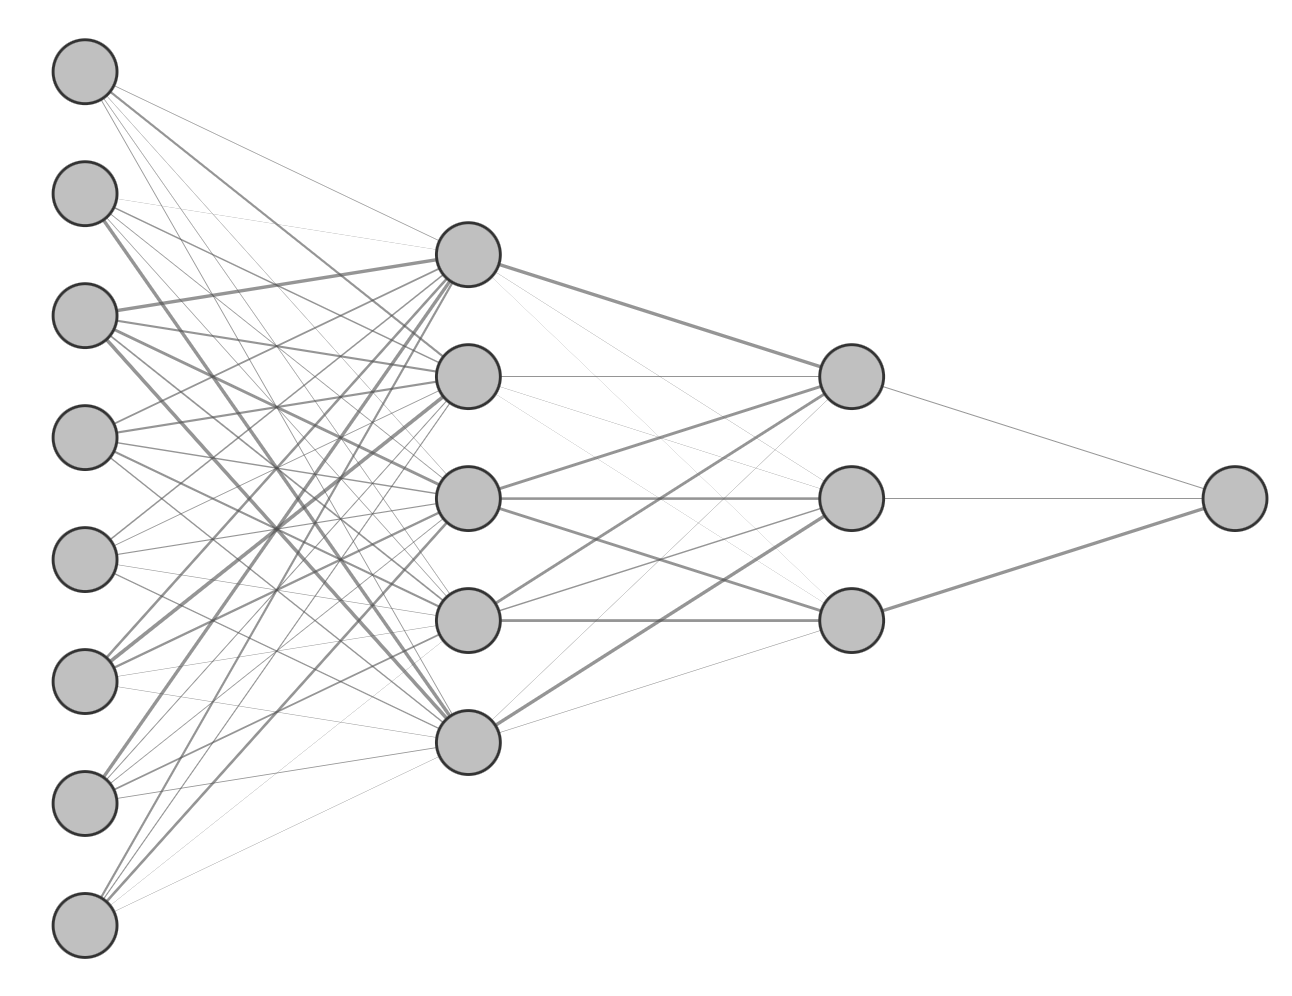
\includegraphics[width=0.8\linewidth]{Images/useful figures/nn_arch.png}
    \caption[Example structure of deep neural network]{Example structure of a deep neural network architecture comprised of an input layer, two hidden layers, and an output layer. The weights on each connection are represented by the intensity of the line the nodes.}
    \label{fig:nn_arch}
\end{figure}

Neural networks are typically funnel-shaped, reducing high-dimensional data to a lower dimensional representation as information is passed through the layers. 
The nodes in a single layer are connected to each node in the adjacent layers via weights, which are iteratively updated in order to reproduce the behavior of the data pushed through the network throughout the training process. 
The nodes receive a signal from either the input (at the input layer) or from connected nodes, which varies in intensity depending on the weight of the connection.
Higher-weighted connections have a stronger influence over the activation of the subsequently connected node.
The signal input to a node passes through a nonlinear activation function, which transforms the weighted-sum of all inputs from the previous layer into some output value.

The connections between neural network nodes can be expressed with a simple mathematical formulation, shown in Eqn. \ref{eq:nn_eqn}, where the output value $y$ is obtained from the weighted (by $w_i$) sum of inputs $x_i$, which is often (though not always) adjusted with a bias value $b$. 

\begin{equation}
y = \sum_{i}^{n} (w_i x_i) + b
\label{eq:nn_eqn}
\end{equation}

For the input and hidden layers, this value is passed onto the next layer, where the same operation takes place.
The output layer produces a prediction value for the given input, though sometimes the output value undergoes one last transformation to shift into the range of values expected by the data used in training.

The size and shape of neural networks greatly influence their ability to capture complex behavior in chemical systems.
Shallow networks with few neurons are excellent tools for learning the patterns in low-dimensional data, but many interacting chemical species require an increasingly broad and deep network size to learn the landscape of possible chemical interactions.
However, larger network sizes are not necessarily better: excessively deep neural networks are more costly to train and increase risks of overfitting, while networks with too many neurons expect higher-dimensional behavior than the interactions captured in the training data.
Balancing the size of networks with the complexity and scope of the data used in training is vital for designing model architectures that achieve the accuracy and efficiency that has become synonymous with interatomic neural network potential (NNP) models. 

Supervised training of ML models involves iteratively passing data through the networks and asking the model to predict a desired property of the data.
This output prediction is compared to a reference value, as training data is labeled, and the predictive error is computed to weigh in the loss, or cost, function which determines how much the weights need to update in order to better capture the behavior represented in the training data. 
In interatomic potential models, at least within the scope of the work presented here, the labeled data is \textit{ab initio} computations of molecular energy and the forces acting upon atoms within a molecular conformation.
The weights are updated via a fine-tuning process known as backpropagation, which uses a stochastic gradient descent optimizer such as Adam \cite{adam_optim} to change the weights based on the gradients of the loss function at each training iteration. 
Another important hyperparameter used in training neural network models is the learning rate, which controls the step size in weight adjustments.
Learning rate plays an important role in reaching convergence when training: a large value can prevent the model from reaching stable predictions, while low learning rates can slow the training process and lead to increased computational costs to reach converged behavior.

Achieving broad generalizability of chemical systems requires large quantities of carefully crafted training data.
Training efficiency can be increased by batching data into smaller segments, which helps the model learn the relationship between molecular structure and the desired predicted properties without specifically memorizing individual pieces of the training data, which we refer to as overfitting.
The choice of training data greatly impacts the ability of a model to extrapolate between conformational and configurational relationships observed in training with the novel use cases encountered in inference. 
Without representing generalized behavior in the training data, a model will be unable to represent generalizable performance and applicability.
Section \ref{subsec:Data quality and availability} explores the importance of comprehensive training data in the development of ML models.

\subsection{Data Quality and Availability}
\label{subsec:Data quality and availability}

Statistical learning models are bounded in accuracy by the quality and quantity of data used in training. 
Many applications of machine learning, such as computer vision, have an abundance of data available for training a model to artificially reproduce. \cite{deep_learning_lecun}
In computational chemistry, however, the object is largely to explore and model behavior that is not understood well, meaning the data which describes phenomena of interest is often sparce and must be generated specifically \cite{ml_energy_conserving_ff_chmiela, pes_fitted_by_NN_handley, ab_initio_pes_using_ml_lu, protein_ff_fragmentation_nn_wang, PES_gasphase} for use in training a learning model to reproduce the physical behavior of systems of interest. 

Data quality is an abstract and difficult to define concept.
In the context of chemical simulation, high-quality data encompasses the accuracy of the underlying physics utilized, as well as the diversity of chemical environments modeled.
Ideally, a properly constructed ML interatomic potential model can learn to represent any dataset, though in practice this is difficult to achieve.
Chemical space is immense, and could be considered practically infinite; up to $10^{60}$ organic molecules \cite{chemical_space} fall into the space loosely defined by Lipinski's rule of five \cite{lipinski} for druglike molecules.
Curating a dataset which represents all possible behavior even limited to this subsection of chemical space is challenging due to the vast possibilities in configurational and conformational diversity.

Poor-quality data can lead to systematic errors in learned potential energy landscapes, reducing the reliability and transferability of ML potential models.
Deficiencies in data quality arise from many factors including, but not limited to: the approximations made in one's choice of \textit{ab initio} theory, which become a source of error in computed molecular energy and atomic forces; limited sampling of conformational and configurational chemical space, restricting the exposure of varied chemical environments to the model; and biases in data selection, which can lead to an overrepresentation of chemical motifs and skew predictive capabilities or lead to overtraining.
Addressing these challenges requires careful dataset curation to capture the accuracy of the underlying physics represented in training data with broad coverage of relevant chemical environments.

The accuracy of reference data labels is vital to the fidelity of an ML model. 
In NNP models trained on \textit{ab initio} molecular energy computations this corresponds to the level of quantum theory utilized in generating the training data, such as DFT \cite{dft_first_paper} or coupled-cluster \cite{coupled_cluster_first_paper} methods.
Lower-level methods introduce approximation errors that will be learned by the model, whereas higher-level, more chemically accurate methods are too computationally prohibitive to apply to large systems or for generating vast quantities of data.
One possible solution to this trade-off is the use of transfer learning, where the base-level physics are learned from lower-level theory, and the model is later fine tuned with a small subset of data produced by more computationally expensive methods.
Applications of transfer learning are discussed in greater detail in Subsection \ref{subsec:ANI_datasets}.

Beyond the accuracy of reference data, diversity plays an integral role in the robustness of a model.
Datasets limited to a narrow region of chemical space---\textit{e.g.}, only sampling equilibrium geometries or from a small subset of chemical species---will result in less generalizable inference performance when encountering unseen molecular structures, despite reporting low errors during testing and validation.
Conformational sampling of molecular structures in off-equilibrium geometries is relatively straightforward, requiring the identification of regions of chemical space where model uncertainty is highest and distorting bond angles and distances around those regions.
This type of sampling is widely used in active learning approaches to generating data that fills gaps in ML model understanding.
Sampling new molecular configurations via active learning is more involved; after identifying high-uncertainty predictions, new structures must be strategically selected to include underrepresented chemical motifs.

In addition to the quality of data used in building training sets, one must consider the availability of that data.
For ML interatomic potentials trained on QM energies, data availability pertains to the feasibility of generating large datasets of molecular properties, where molecular size and atomic complexity are the limiting factors to computing vast amounts of data at sophisticated levels of theory.
Public datasets of first-principles calculations \cite{qm9, qm40} help to mitigate this limitation, though these are the result of ongoing efforts to expand the availability of high-accuracy quantum chemical data.

This consideration is further applicable to tools used to predict experimental results such as NMR chemical shifts \cite{shiftx, legolas} from structural geometries.
For example, the neuraL nEtwork enGine fOr caLculating chemicAl Shifts (LEGOLAS) \cite{legolas} gives rapid, accurate predictions of NMR chemical shifts for backbone atoms of proteins, making it a useful approach to structure elucidation and validation in molecular biology.
However, like all ML models, its performance is intrinsically tied to the quality and availability of training data.
LEGOLAS exhibits high accuracy for well-represented chemical environments, but shows poor inference performance on atoms in residues with sparse (or high-uncertainty) training data.
This highlights a fundamental obstacle in machine-learned predictions of chemical systems: achieving reliable generalization requires datasets that comprehensively capture the vastness of chemical space that could be encountered in real-world applications.

The interplay between data availability and quality with the transferability of a fully-trained ML model highlights the importance of dataset curation for developing a generalized ML interatomic potential model.
The broader implications of data limitations extend to various chemical applications, from force field development, modeling of chemical reactions, and prediction of molecular properties.
The ability of ML models to generalize behavior across the complexity of chemical space remains a challenge, though exemplary models have shown success in producing high-accuracy predictions.
One such example is explored in Section \ref{sec:ANI_intro}, which will remain the focus of the work presented in the subsequent chapters, and serves as a case study for understanding how neural network potentials can be applied to streamlining energy calculations at quantum-levels of accuracy, as well as the simulation of reactive chemical environments.


\section{The Artificial NeurAl networK engINe for Molecular Energies: ANI}
\label{sec:ANI_intro}

Within the realm of machine learning in chemistry and neural network potentials, the Artificial NeurAl networK engINe for Molecular Energies (ANAKIN-ME or, more commonly, ANI) \cite{ani-1} was a landmark development in potential energy surface predictions.
Building on the foundations set by earlier NNP models, such as HDNN \cite{behler_parrinello} by Behler and Parrinello, ANI-1 used an atom-specific neural network architecture to predict molecular energies with chemical accuracy comparable to density functional theory at a speedup of approximately $10^6$.
Implemented in a C++ and CUDA program called NeuroChem, ANI-1 was trained on a dataset \cite{ani-1_dataset} of 17.2 million small organic molecules containing only hydrogen, carbon, nitrogen, and oxygen atoms. 
Despite the training set containing only up to 8 heavy (non-hydrogen) atoms, the model performed well on test sets of 10-24 atoms---within 1 kcal/mol of the DFT reference energy for near-equilibrium structures \cite{ani-1}.
ANI-1x \cite{ani-1x} and 1ccx \cite{ani-1ccx} were introduced as an improvement over ANI-1 by leveraging smaller, more carefully crafted datasets to achieve greater accuracy, generalization, and scalability; the cultivation of these datasets is explored in Subsection \ref{subsec:ANI_datasets}.
Figure \ref{fig:accuracy-cost} qualitatively demonstrates how the various published ANI models perform against routinely applied methods in computational chemistry, showcasing that ANI is capable of predicting molecular energies with first-principles levels of accuracy at approximately the same cost as force field methods.

\begin{figure}[!ht]
    \centering
    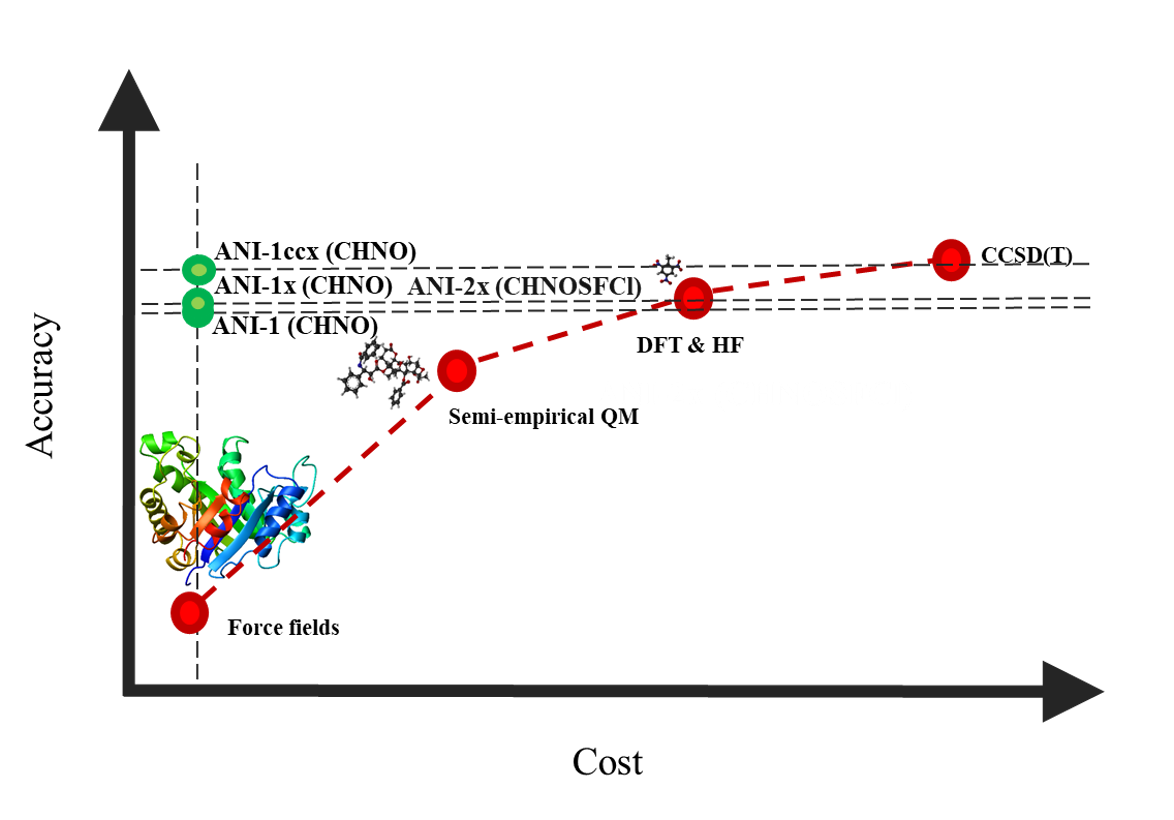
\includegraphics[width=1\linewidth]{Images/accuracy-cost.png}
    \caption[Approximate scaling of compute time versus chemical accuracy in various computational chemistry methods]{
    Approximate scaling of compute time versus chemical accuracy in various computational chemistry methods. Neural network potential models in the TorchANI package compute energies at DFT (or greater) levels of accuracy, at a cost similar to that of force fields.
    }
    \label{fig:accuracy-cost}
\end{figure}

The ANI methodology was further extended to sulfur, fluorine, and chlorine with the release of ANI-2x \cite{ani-2x, 2x_dataset} and implemented in Python using the PyTorch library \cite{pytorch} in the TorchANI package \cite{torchani}.
With these advancements, and adaptations to traditional QM/MM embedding approaches for boundary atoms, the ANI-2x potentials have been applied to hybrid ML/MM schemes \cite{ml_mm_galvelis, ml_mm_santi_y_jonny1, ml_mm_santi_y_jonny2}.
ANI-style networks have also proven useful in rapid, parallelized predictions of NMR chemical shift ($\delta$) values for protein backbones \cite{legolas, torchani}, particularly in their application in molecular dynamics simulations.
Reactive potentials such as ANI-1xnr \cite{ani-1xnr} further extend the predictive capabilities of ANI neural network potentials; refer to \ref{subsec:ANI_datasets} for details on the dataset used in training this reactive potential.

To better understand the ANAKIN-ME methodology, we must look more closely at a few aspects: the descriptor, Atomic Environment Vectors; the structure of ANI neural networks; and the datasets used for training, validating, and testing ANI models.

\subsection{The Atomic Environment Vector}
\label{subsec:AEV}

A fundamental component of the predictive accuracy of ANI models is the construction of the Atomic Environment Vector (AEV) \cite{ani-1}, which provides a systematic approach to encoding local atomic interactions.
Using the modified BP symmetry functions \cite{behler_parrinello} given in Equations \ref{eq:radial_symmetry_function} and \ref{eq:angular_symmetry_function} within a specified cutoff radius---5.2 \angstrom for the radial component and 3.5 \angstrom for the angular component---an atom-centered representation of the local chemical environment is constructed into a fixed-length vector.
An example of the angular AEV radius is given in Figure \ref{fig:aev_radius}.
The leftmost image shows the molecule used in the example, while the middle image is a demonstration of the cutoff radius, and the rightmost image shows how atoms outside of this radius are not seen by the atom an AEV is being constructed for.

\begin{figure}[h!]
    \centering
    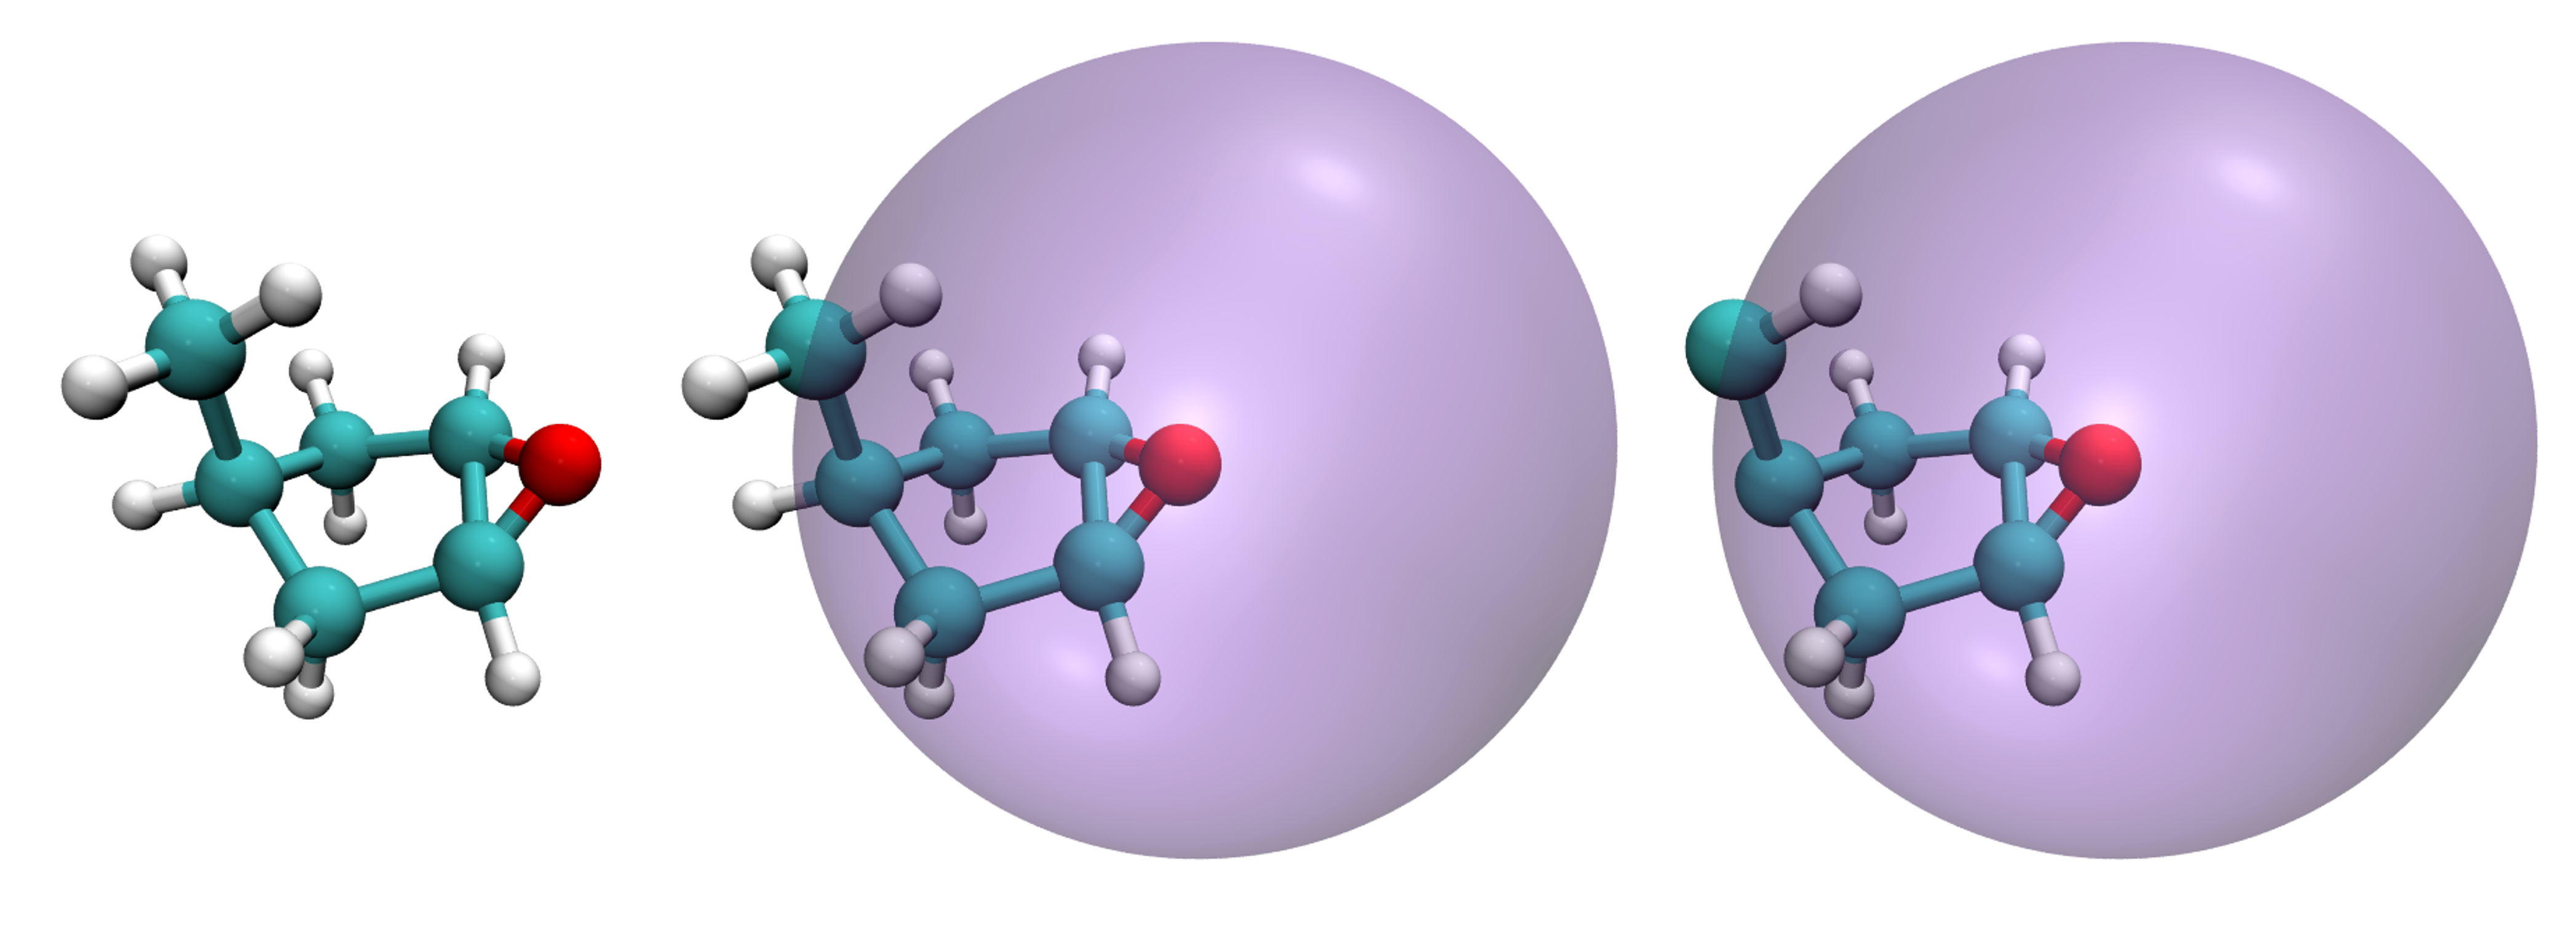
\includegraphics[width=1\linewidth]{Images/aev_radius/aev_radius_combined.png}
    \caption[Demonstration of AEV angular cutoff radius.]{Angular cutoff radius for the oxygen in C$_6$H$_{10}$O. Note that three hydrogen atoms fall outside of the cutoff radius, making them effectively invisible to the oxygen atom.}
    \label{fig:aev_radius}
\end{figure}

As described in Subsection \ref{subsec:ML_atomic_representation}, the radial component embeds two-body interactions based on distances between atoms, while the angular component embeds three-body interactions for all possible pairs of neighboring atoms.
This representation is designed to be rotationally, translationally, and permutationally invariant, meaning that chemically equivalent atoms are treated consistently regardless of their spatial orientation or ordering within the molecular structure.
Unlike Behler-Parrinello symmetry functions, the AEV computer utilized in the ANI methodology incorporates information about the atom types (elements) encoded in the atomic representation, which in turn yields lower-error predictions on multi-molecule training sets and permits better transferability \cite{ani-1}.
Figure \ref{fig:aev_construction} is a schematic representation of the AEV construction. 
For a full list of parameters used in the TorchANI AEV computer, see Appendix \ref{appendix:AEV_param}.

\begin{figure}[hb]
    \centering
    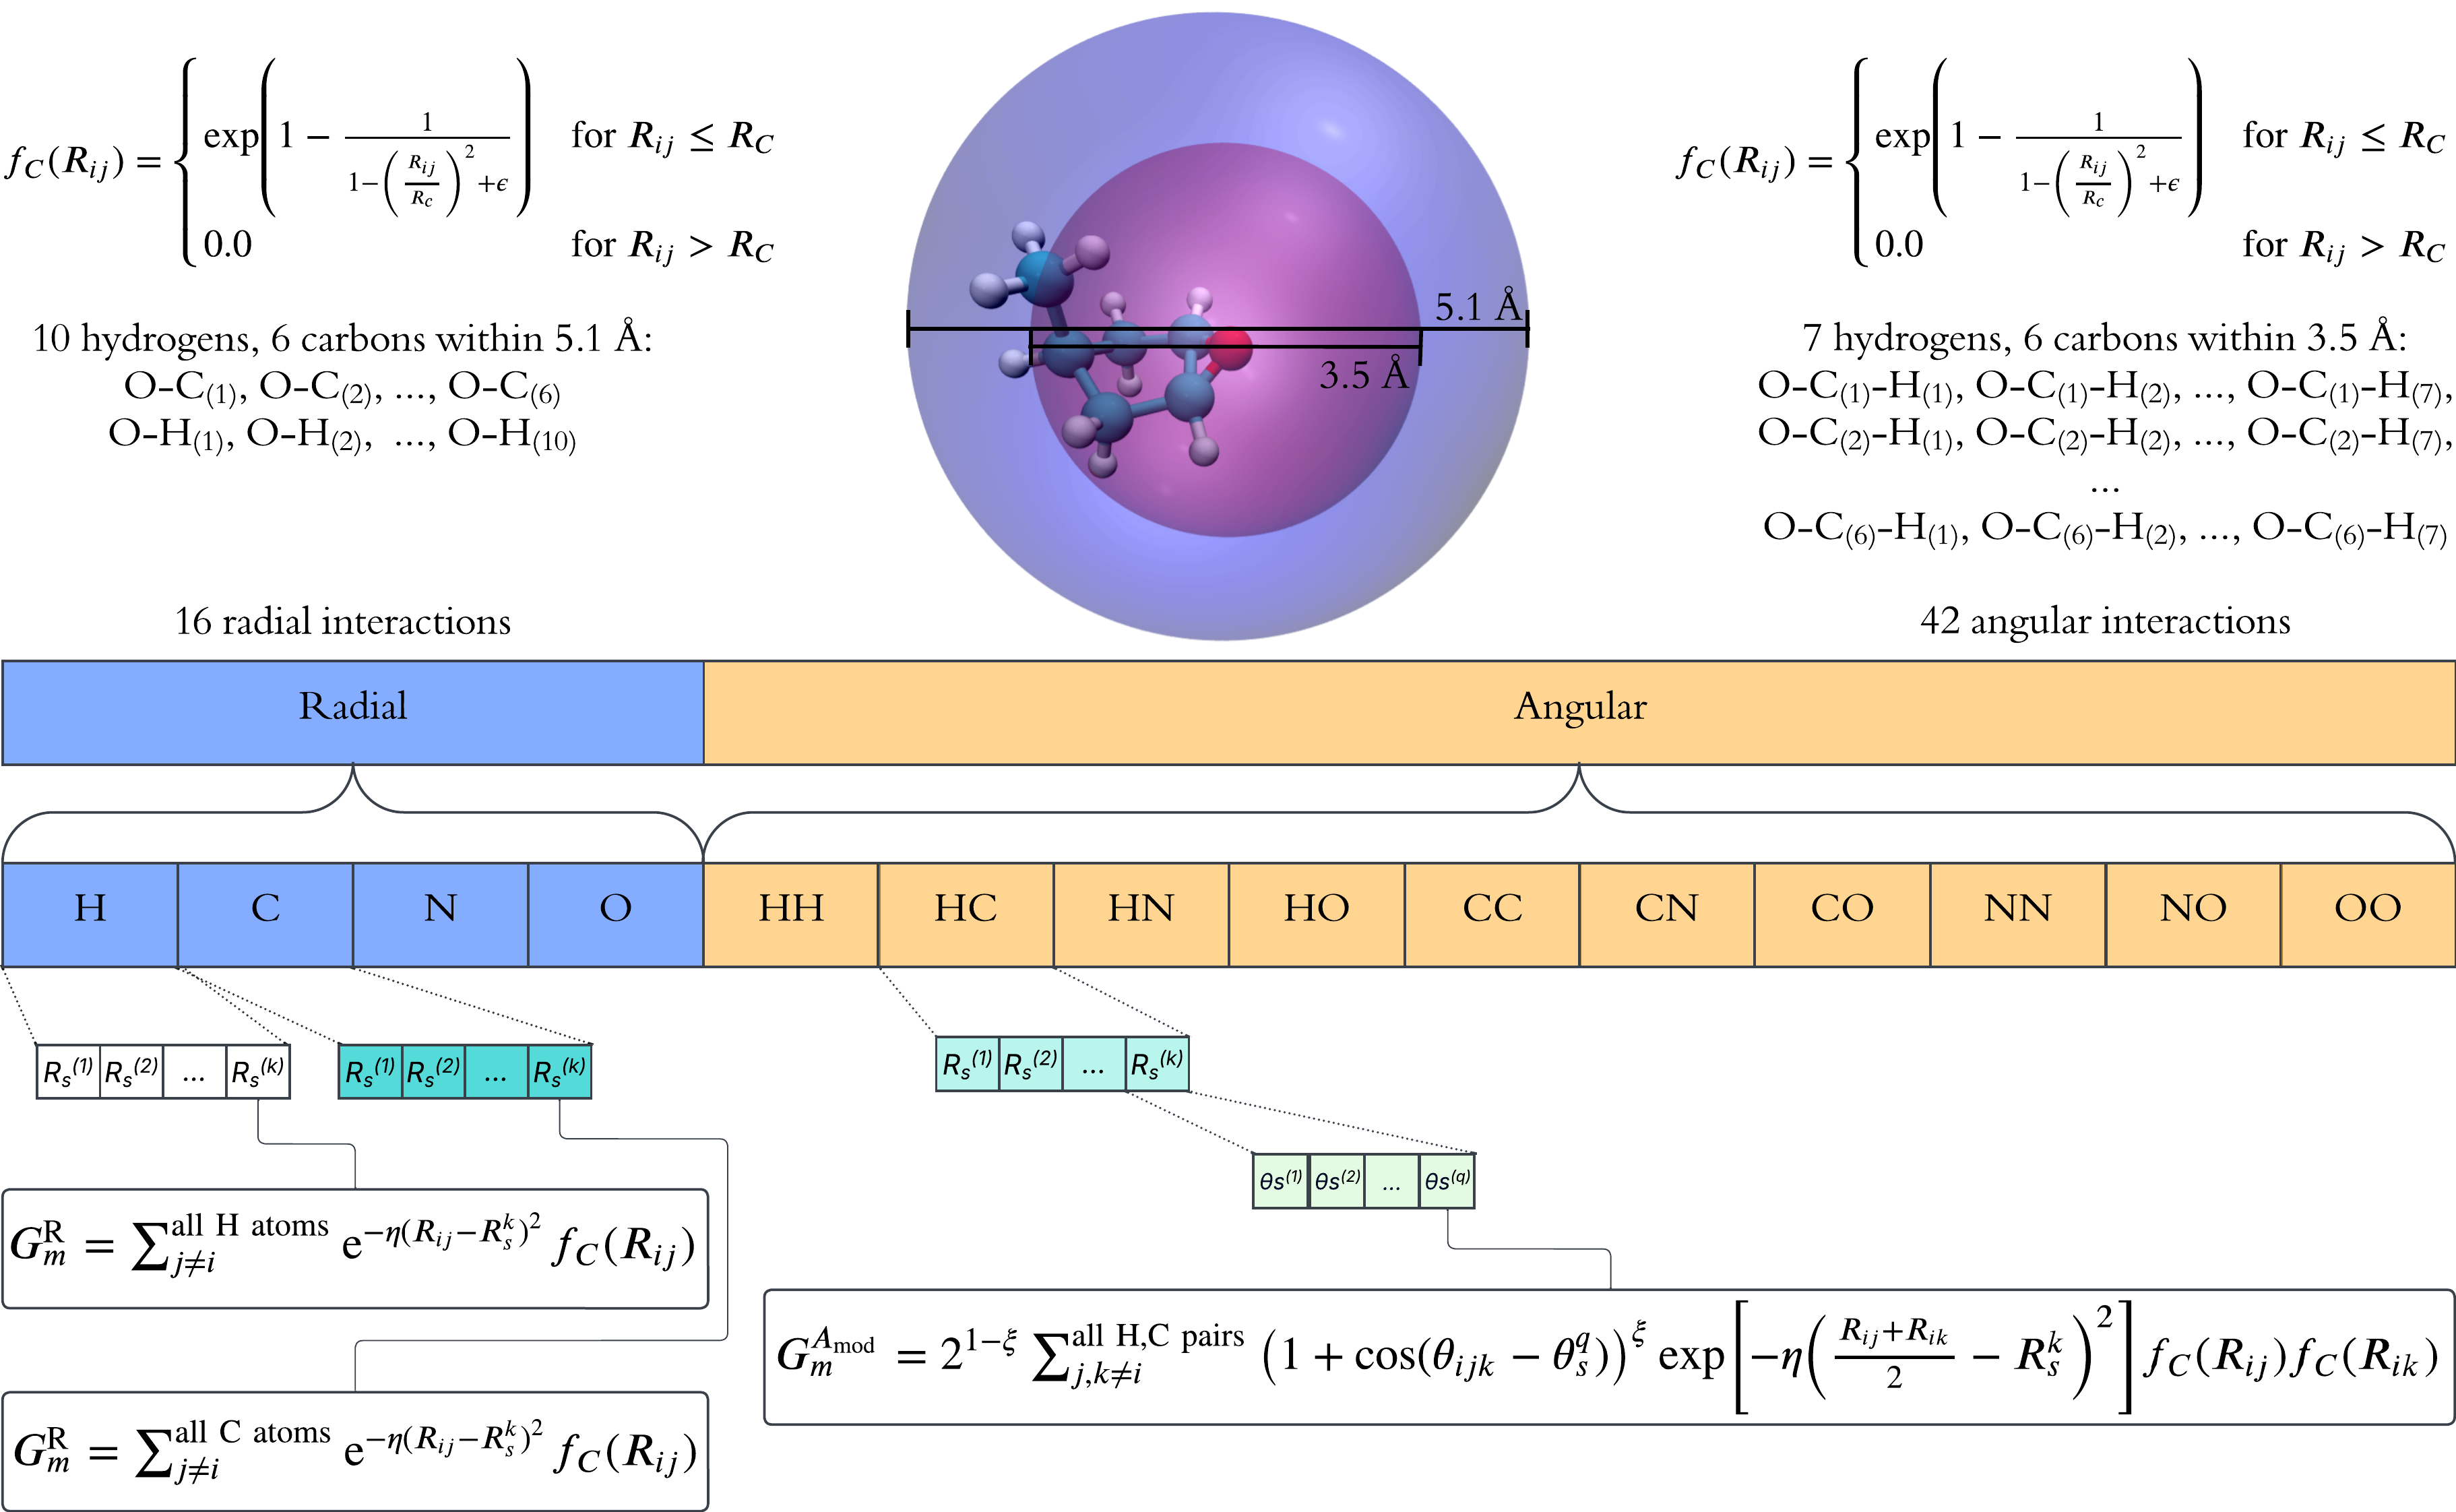
\includegraphics[width=1\linewidth]{Images/aev_radius/AEV_construction.png}
    \caption[Example of atomic environment vector construction]{Example of the terms in an AEV for the lone oxygen in the C$_6$H$_{10}$O molecule used in Fig. \ref{fig:aev_radius}.}
    \label{fig:aev_construction}
\end{figure}

During training and inference, AEVs serve as the inputs to element-specific neural networks, where they are used to predict the contribution of each atom to the total molecular energy.
This relationship is explored in detail in Subsection \ref{subsec:total_E_sum_AEs}.
The scalability of ANI predictions is due to this representation of local atomic environments and, though it neglects long-range interactions, does well to predict molecular energies for systems much larger than those included in the training sets \cite{ani-1x, ani-2x}.

The use of a robust descriptor is vital to creating a generalized representation of chemical environments, and serves as the basis for modeling chemical behavior.
However, a robust descriptor is just one component of a successful ML model; the neural network architecture built around these descriptors enable efficient learning of the chemical relationships in QM data.
The following section explores the architecture of ANI models, and how the fixed-length AEV is used as an input to produce predictions of molecular energy.


\subsection{ANI Model Architecture}
\label{subsec:ANI_model_arch}

The ANI models use a modular neural network architecture, where each unique atom type employs a species-specific feedforward network to learn the relationships between local atomic environment and the contribution of each atom in the system to the total molecular energy.
This energy decomposition makes it possible for ANI to efficiently scale to systems outside of the scope of the training data. 
Each of the species-specific networks are similar in structure, containing the same number of neurons in the input layer but employ different hidden layer shapes due to variations in atomic bonding and dataset composition.
Full network specifications for ANI-1x and 2x-like networks are provided in Appendix \ref{appendix:NN_arch}.

The hidden layers transform the input AEV into a high-dimensional latent feature space where patterns in atomic interactions and energy can be learned effectively.
The input signal undergoes dimensional reduction with each hidden layer, becoming more abstract to capture nonlinear, chemically relevant patterns in the data input to the network. 
This funnel-shaped network structure, combined with the robust descriptor detailed in Subsection \ref{subsec:AEV}, are key in the ability of ANI models to make generalized predictions beyond the training dataset.

Neural networks are highly flexible, and can learn to predict properties of unseen data based on trends in the, often, very high-dimensional data used in training.
Supervised training, as mentioned in Subsection \ref{subsec:ML_model_architecture}, is the iterative optimization process of updating the weights connecting nodes in neural networks to minimize the error between predicted and labeled data.
This optimization is based on the output of a loss function.
For ANI models, the most basic chemical property trained to is the total molecular energy.
The predictive error of an ANI model is minimized in training using a mean squared error loss function that quantifies the difference between predicted molecular energy and the QM reference values.
An example of the energy loss function utilized in training a typical ANI model is given in Eqn. \ref{eq:energy_loss_function}.

\begin{equation}
    \mathcal{L}_{\text{2x}} =
    \frac{1}{N_{\text{M}}} 
    \sum_{i=1}^{N_{\text{M}}} 
    \left( \frac{ \left( E_{\text{ANI}}^\text{o} - E_{\text{QM}}^\text{o} \right)^2}
    {\sqrt{N_{\text{atoms}}}} \right)
    \label{eq:energy_loss_function}
\end{equation}

Here, $E_{\text{ANI}}^\text{o}$ is the molecular energy predicted by the ANI model and $E_{\text{QM}}^\text{o}$ is the reference QM energy; the atomic self-energies (discussed further in \ref{subsec:total_E_sum_AEs}) are excluded from these values.
The computed mean square error is normalized by the atom count ($N_{\text{atoms}}$) of the system such that large systems do not dominate the computed loss.
Loss is computed in the forward pass for a batch of $N_{\text{M}}$ molecules and the result of this function is used in the backward pass with the Adam optimizer \cite{adam_optim} to determine how dramatically the weights are updated for the next training iteration in order to make energy predictions more closely match the reference values, minimizing the loss calculated for each batch of molecules. 
This process of iteratively updating weights is called backpropagation.
Batching data into small (relative to the overall dataset) segments allows backpropagation to be accelerated by efficiently updating the weights of each network based on a representative subset of molecules. 

Flexible neural network architecture, along with the reliablity of AEV descriptors as the input to harness the power and efficiency of NNPs, enable ANI models to be scalable to large systems and provide generalized representations of atomic interactions within molecules.
There is still, however, one important aspect of the ANAKIN-ME methodology to explore: the dataset used in training, which is crucial to the transferability of ANI models.


\subsection{The ANI Datasets}
\label{subsec:ANI_datasets}

Machine-learned models perform, at best, to the limit of the data used in training.
Creating a generalized dataset of organic molecules and chemically accurate energies is the most complex and computationally prohibitive aspect of an accurate ML interatomic potential model.
The ANI-1 dataset \cite{ani-1_dataset} contained 57,951 unique molecular configurations from the GDB-11 enumeration dataset \cite{gdb-11-1, gdb-11-2}, with conformational sampling pushing this to over 17 million structures.
Calculating QM single-point energies for all structures in the dataset is highly taxing, and would require that a trained model is extremely versatile to justify the tremendous computational expense; a more efficient data selection approach was necessary to extend the applicability of the model further.

The ANI-1x potential \cite{ani-1x} was introduced as an improvement over ANI-1 by leveraging active learning to expand the chemical space explored in the ANI dataset by focusing on regions where the model exhibited high uncertainty. 
The ANI-1x dataset \cite{1x_1ccx_datasets} was generated from a subset of ANI-1, achieving lower energy RMSE predictions with a quarter of the data \cite{ani-1x}. 
This was described as a ``less is more" approach, where the inclusion of highly informative training data led to a greater reduction in error than simply increasing the dataset size indiscriminately.
In order to generate new conformational data from the initial ANI-1 configurations, four techniques were employed: molecular dynamics sampling, normal mode sampling, dimer sampling, and torsion sampling. 
These are excellent approaches to generating new conformational data, but fall short in the uncertainty metric used in deciding what data is performing poorly.
The deficiencies of this approach to data sampling are further explored in Chapters \ref{chapter2} and \ref{chapter3}. 

Along with ANI-1x, a transfer learning approach to approximating coupled-cluster calculations was developed: ANI-1ccx \cite{1x_1ccx_datasets}. 
By selecting only 10\% of the molecular conformations in the ANI-1x dataset---recomputed with MP2/(aug-)cc-pV[TQ]Z \cite{1ccx_ccsd(t)} extrapolation and CCSD(T) correlation energy corrections with the (aug-)cc-pVTZ \cite{1ccx_basis} basis set---ANI-1ccx predicts energies at approximately CCSD(T) levels of accuracy $10^9$ faster than full CCSD(T) calculations.
Utilizing the same active learning scheme with data from the GDB-13 \cite{gdb-13} and GDB-17 \cite{gdb-17} enumeration datasets, the ANI-2x dataset was produced to include sulfur, fluorine, and chlorine.
The selection of just seven elements (H, C, N, O, S, F, and Cl) increases the applicability of ANI from the limited subset of small organic molecules to encompass 90\% of all druglike molecules \cite{ani-2x}.

Published ANI models \cite{ani-1, ani-1x, ani-2x} are primarily trained on data computed at the $\mathrm{\omega}$B97X level of density functional theory \cite{wB97X} with a 6-31G* basis set \cite{6-31g*}, which provides a balance of moderate chemical accuracy at reasonable computation speeds.
The average time for a single-point energy prediction with ANI-2x is approximately 0.02 seconds, while the training data required an average of 552 seconds per single-point calculation \cite{ani-2x}.
Table \ref{tbl:dataset_sizes} contains dataset sizes, purposes, and details about the composition of each of the published ANI datasets.
Specialized datasets for in-house use are not considered in the work presented here, though other datasets have been created for unique purposes.

\begin{table}[!ht]
\centering
\caption[Datset sizes for ANI-1, 1x, 1ccx, 2x, COMP6v1, and COMP6v2]{
Dataset sizes for ANI-1, 1x, 1ccx, 2x, COMP6v1, and COMP6v2.
Selected conformer counts are for data available at the $\mathrm{\omega}$B97X level of theory with a 6-31G* basis set, with the exception of the ANI-1ccx dataset.
Datasets listed here are available at other levels of theory, though $\mathrm{\omega}$B97X is the only data specifically referenced in this dissertation.
}
\label{tbl:dataset_sizes}
    \begin{tabularx}{\textwidth}{{l r l p{7.4cm}}}
      \hline
      Dataset & \# conformers & Utility & Note \\
      \hline
      ANI-1 & 17,216,350 & Original training set & Sampled from 57,951 unique molecules; up to 8 heavy atoms \\
      ANI-1x & 4,956,005 & 1x-like training set & Sampled with active learning from ANI-1; up to 63 atoms\\ 
      ANI-1ccx & 489,515 & Transfer learning set & Sampled with active learning from ANI-1x; up to 55 atoms \\
      ANI-2x & 9,651,712 & 2x-like training set & Includes all 1x conformers plus compounds containing S, F, Cl; up to 63 atoms \\
      COMP6v1 & 101,352 & 1x-like testing set & Benchmark data $\notin$ training sets; up to 312 atoms \\ 
      COMP6v2 & 157,728 & 2x-like testing set & Includes all of COMP6v1 plus molecules containing S, F, Cl; up to 312 atoms \\
      \hline
    \end{tabularx}
\end{table}

Specialized datasets for use with ANI-styled networks have pushed the boundaries of machine-learned interatomic potentials; ANI-1xnr \cite{ani-1xnr}, for example, was developed to model reactive potential energy surfaces, incorporating transition state geometries into the training data to improve predictive accuracy for bond-breaking and bond-forming processes.
Such models have demonstrated significant improvements in modeling molecular reactivity, making them useful in studying chemical reactions---notably prebiotic chemistry, as discussed in Chapters \ref{chapter4} and \ref{chapter5}.



% Modified from old template.
\chapter{Exploration of atomistic predictions}
\label{chapter2}

Atomic interactions are the foundation on which many ML models---especially interatomic potential models---are built.
Accuracy is well-defined in quantum chemical methods via systematic convergence and comparison to experimental data, but wavefunction-based approaches are computationally expensive and are limited to system sizes of only a handful of atoms.
Measuring predictive accuracy is difficult when approximating the results of first principles computations for systems that exceed the size limitations of QM approaches.
This raises a vital question to the efficacy of ML models: how do we assess the reliability of atomistic neural network potential models for systems that exceed the size limitations of QM computations?

The scalability of NNP models stems from partitioning molecules into atomic components, characterized by their local chemical environment.
However, this introduces new challenges in generalization and transferability and, therefore, model reliability when exposed to new atomic interactions during inference.
This chapter serves as an assessment of the reliability of model predictions of molecular enery and atomistic energy contributions in ANAKIN-ME neural network potential models.
Section \ref{sec:ANI_predictions} contains a detailed look at the predictions of ANI neural networks from atomistic features to global properties and the measure of uncertainty used to determine the trustworthiness of a prediction.
The following section, \ref{sec:uncertainty_atomic_energies}, details the search for an improved metric of reliability in atomistic predictions.

\section{ANAKIN-ME Predictions}
\label{sec:ANI_predictions}

The ANI methodology provides a framework for atom-wise decomposition of molecular energies by using the atomic environment vector (AEV) representation to encode localized chemical interactions.
A decomposition approach allows for efficient, scalable predictions of energy for systems larger than the training data represents.
This is advantageous for simulating large systems, due to the size limitations of \textit{ab initio} computations.
The driving idea behind the AEV representation is that all atomic interactions within a system can be characterized by the localized environment. 
This neglects long-range interactions such as van der Waals forces and electrostatics, which are undoubtedly important for some systems, but has little influence on the predictive accuracy of single-point calculations of small organic molecules.
Corrective approaches to long-range interactions have been explored, such as ANI-MBIS-q \cite{ml_mm_santi_y_jonny2}, which considers long-range electrostatics using a separate, parallel network to predict partial charges.
For small, charge-neutral molecules, localized interactions encoded in the AEV have been shown to capture the relationship between molecular energy and atomic species and their positions \cite{ani-1, ani-1x, ani-2x}.

Though some partitioning schemes exist in quantum theory, such as Bader's Atoms in Molecules \cite{bader_aim}, there is no general consensus for decomposing the energy of a molecular system into a sum of atomic contributions.
The energy decomposition approach taken by ANI is a learned relationship decided by the individual atomic neural networks during training, explained in greater detail in Subsection \ref{subsec:total_E_sum_AEs}.
The uncertainty measure of predicted energies, referred to as the QBC, is defined in Subsection \ref{subsec:ANI_uncertainty}, followed by a case study in Subsection \ref{subsec:flaws_in_qbc} of the reliability of the QBC as a measure of empirical uncertainty in ANI predictions.

\subsection{Molecular Energy as a Sum of Atomic Contributions}
\label{subsec:total_E_sum_AEs}

The predicted molecular energy for a molecule input to an ANI model is computed as a sum of atomic contributions, given in Eqn. \ref{eq:total_E_sum_AEs}, where $E_{\text{Total}}$ is the molecular energy prediction and $\varepsilon_i$ is the atomic energy contribution for atom $i$.

\begin{equation}
    E_{\text{Total}} = \sum_{i}^{\text{atoms}} \varepsilon_i
    \label{eq:total_E_sum_AEs}
\end{equation}

To visualize atomic energy predictions, a small testing subset was created using the first conformer of each molecular formula in the ANI-1x training dataset.
This testing set, referred to as 1x-test ($N=$ 3,114), is used to explore some trends in predicted atomic energies for the carbon, hydrogen, nitrogen, and oxygen atom types across an ensemble of eight models.
Testing on this subset gives insight on the performance of ANI models for well-characterized systems, as this was the data used in training the model.
The ANI-1x and 2x potential models were trained using self-atomic energies (SAEs), where the predicted atomic energy values form a distribution centered at zero. 
This means that, by definition, each atom has either no net contribution to the molecular energy, or contributes an energy deviation that is relative to the baseline for that atom type.
The atomic energy contributions predicted by the ANI-2x model for C, H, N, and O atoms across the 1x-first test set are given in Figure \ref{fig:2x_ae_per_model}.

\begin{figure}[!h]
    \centering
    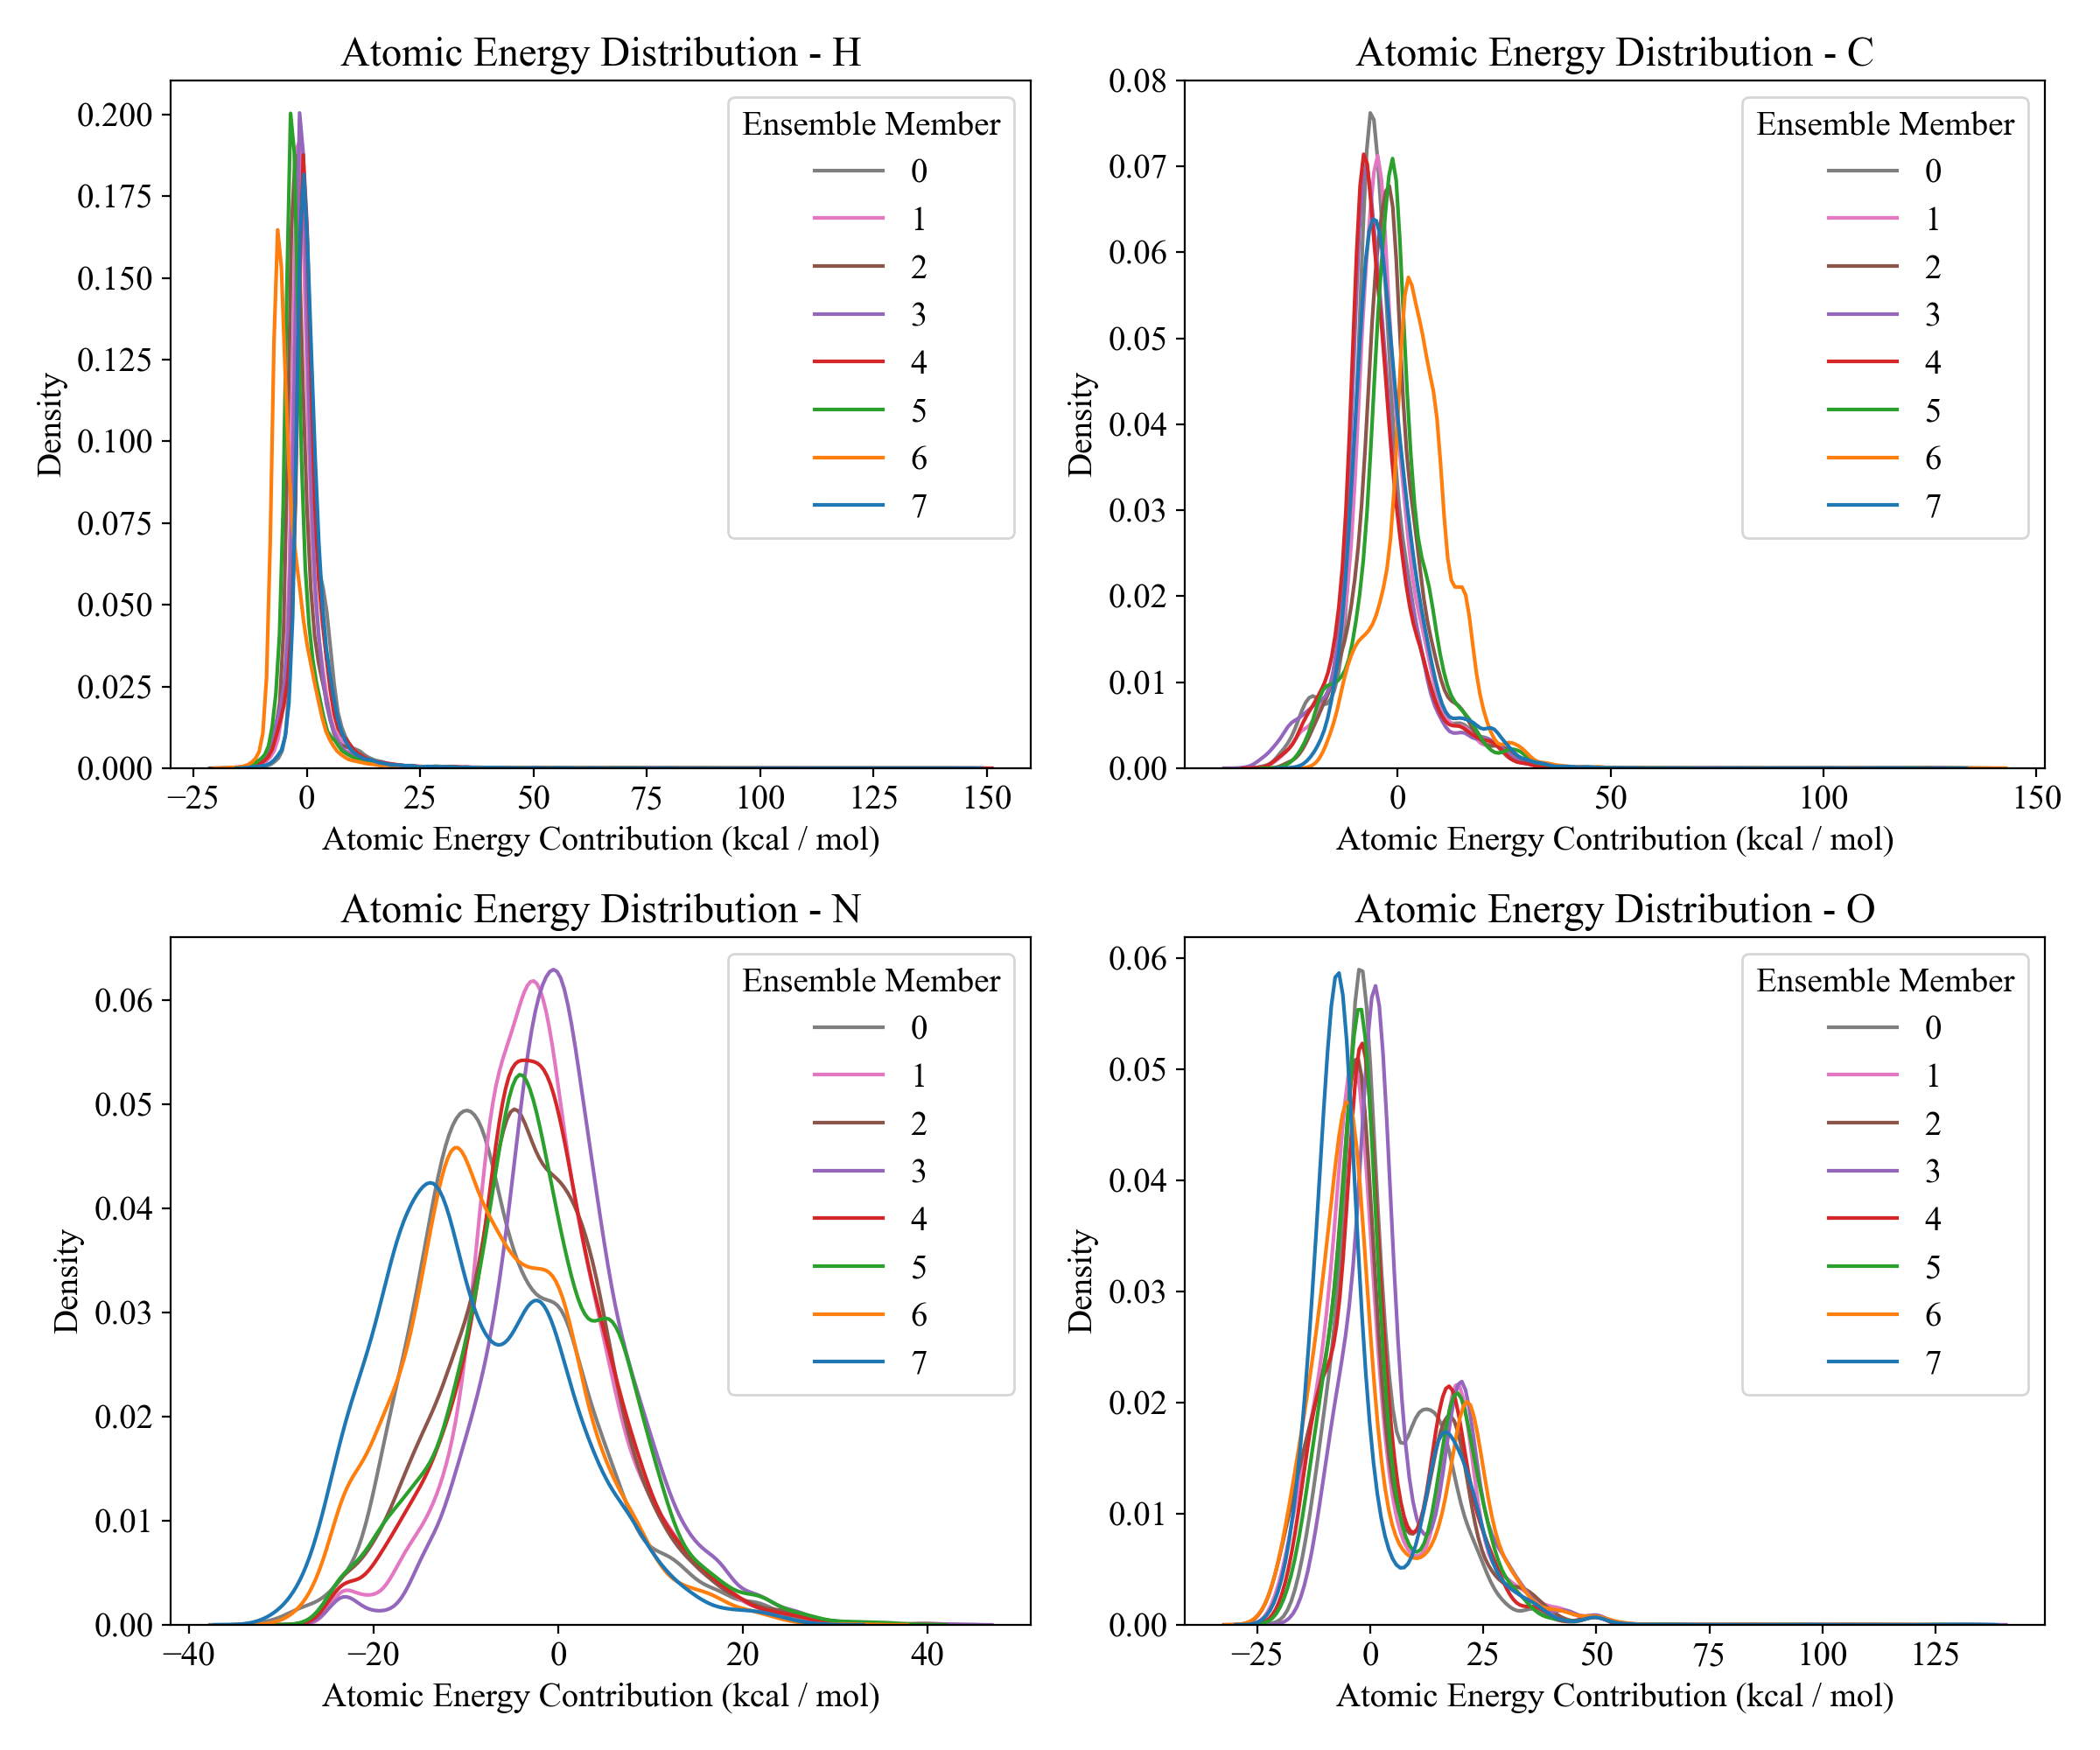
\includegraphics[width=1\linewidth]{Images/2x_outputs/2x_1x-first_ae-per-model.png}
    \caption[Atomic energies predicted by ANI-2x]{Per-model distribution of atomic energy contributions by atom type for the ANI-2x potential. Values shown in kcal/mol for HCNO atom types on the 1x-first subset.}
    \label{fig:2x_ae_per_model}
\end{figure}

Shifting atomic energies with SAEs causes the model to learn relative energy contributions rather than absolute values. 
Refined ANI models, such as ANI-2xr, are trained with slightly different hyperparameters.
The largest change between ANI-2x and 2xr is the removal of biases from neuron outputs; Eqn. \ref{eq:nn_eqn} shows the method for computing the weighted-sum output of each neuron ($y$) from the input ($x_i$) multiplied by its weight ($w_i$).
Traditionally, artificial neural networks use biases to output some value, even when the weighted sum of input values is close or equal to zero.
For interatomic potentials, if we pass a single atom with no neighbors through a network, we would expect to get exactly the energy of that atom in space with no other interacting particles.
By removing the biases from the species-specific networks, we can achieve this goal and add a bit more physicality to the behavior of the neural network outputs.
To replace the biases, we add a final shift to the output: the EnergyShifter.
This is a protocol within TorchANI which adds the ground state atomic energy (GSAE) to each atom, shifting the output values of the NNs toward physically meaningful values.
Ground state atomic energies are calculated at the level of theory used in producing training data from a neutrally charged atom isolated in space with the proper spin multiplicity (ensuring a ground-state electronic configuration).
Thus, the total energy prediction in ANI-2xr networks are computed as shown in Equation \ref{eq:total_E_GSAEs}.

\begin{equation}
    E_{\text{Total}} = \sum_{i}^{\text{atoms}} \varepsilon_i + \text{GSAE}_i
    \label{eq:total_E_GSAEs}
\end{equation}

Here, the total energy is a sum of atomic contributions as in Eqn. \ref{eq:total_E_sum_AEs}, and $\text{GSAE}_i$ is the ground state atomic energy for atom $i$, which shift the network outputs toward more physically meaningful values.
The ground state atomic energies for each atom in the ANI networks are given in \ref{appendix:GSAEs}.
In addition to the removal of biases and the replacement of self-atomic energies with GSAEs, ANI-2xr is trained with the addition of a simple, analytical xTB repulsion term \cite{xtb_repulsion}.
The inclusion of repulsion to the potential introduces more physical behavior in regions of the potential energy surface that are difficult to sample, namely when two atoms get very close together.
Equation \ref{eq:repulsion} shows the form of this repulsion term for two atoms, where $a$ and $b$ (with atomic numbers $A$ and $B$, respectively) separated by a distance $r_{ab}$. 
The parameters $Y_A$ and $Y_B$ define the magnitude of the repulsive term for their respective elements, $\alpha_{A}$ and $\alpha_{B}$ are element-specific parameters, and $k_{AB}$ is a small correction for very light elements (H, He) and equal to 3/2 in all other cases.

\begin{equation}
\label{eq:repulsion}
    E_{\text{rep}}(r_{ab}) = 
    \sum_{AB}\frac{{Y_{A} Y_{B}}}{r_{ab}}
    \exp \left( -\sqrt{\alpha_{A} \alpha_{B}} {(r_{ab})}^{k_{AB}} \right)
\end{equation}

The ANI-2xr atomic energy distribution for hydrogen, carbon, nitrogen, and oxygen are given in Fig. \ref{fig:2xr_ae_per_model} for an eight-membered ensemble.
Note here that the distributions have slightly different shapes, as well as being shifted far from the zero-centered ANI-2x distributions shown in Figure \ref{fig:2x_ae_per_model}.

\begin{figure}[H]
    \centering
    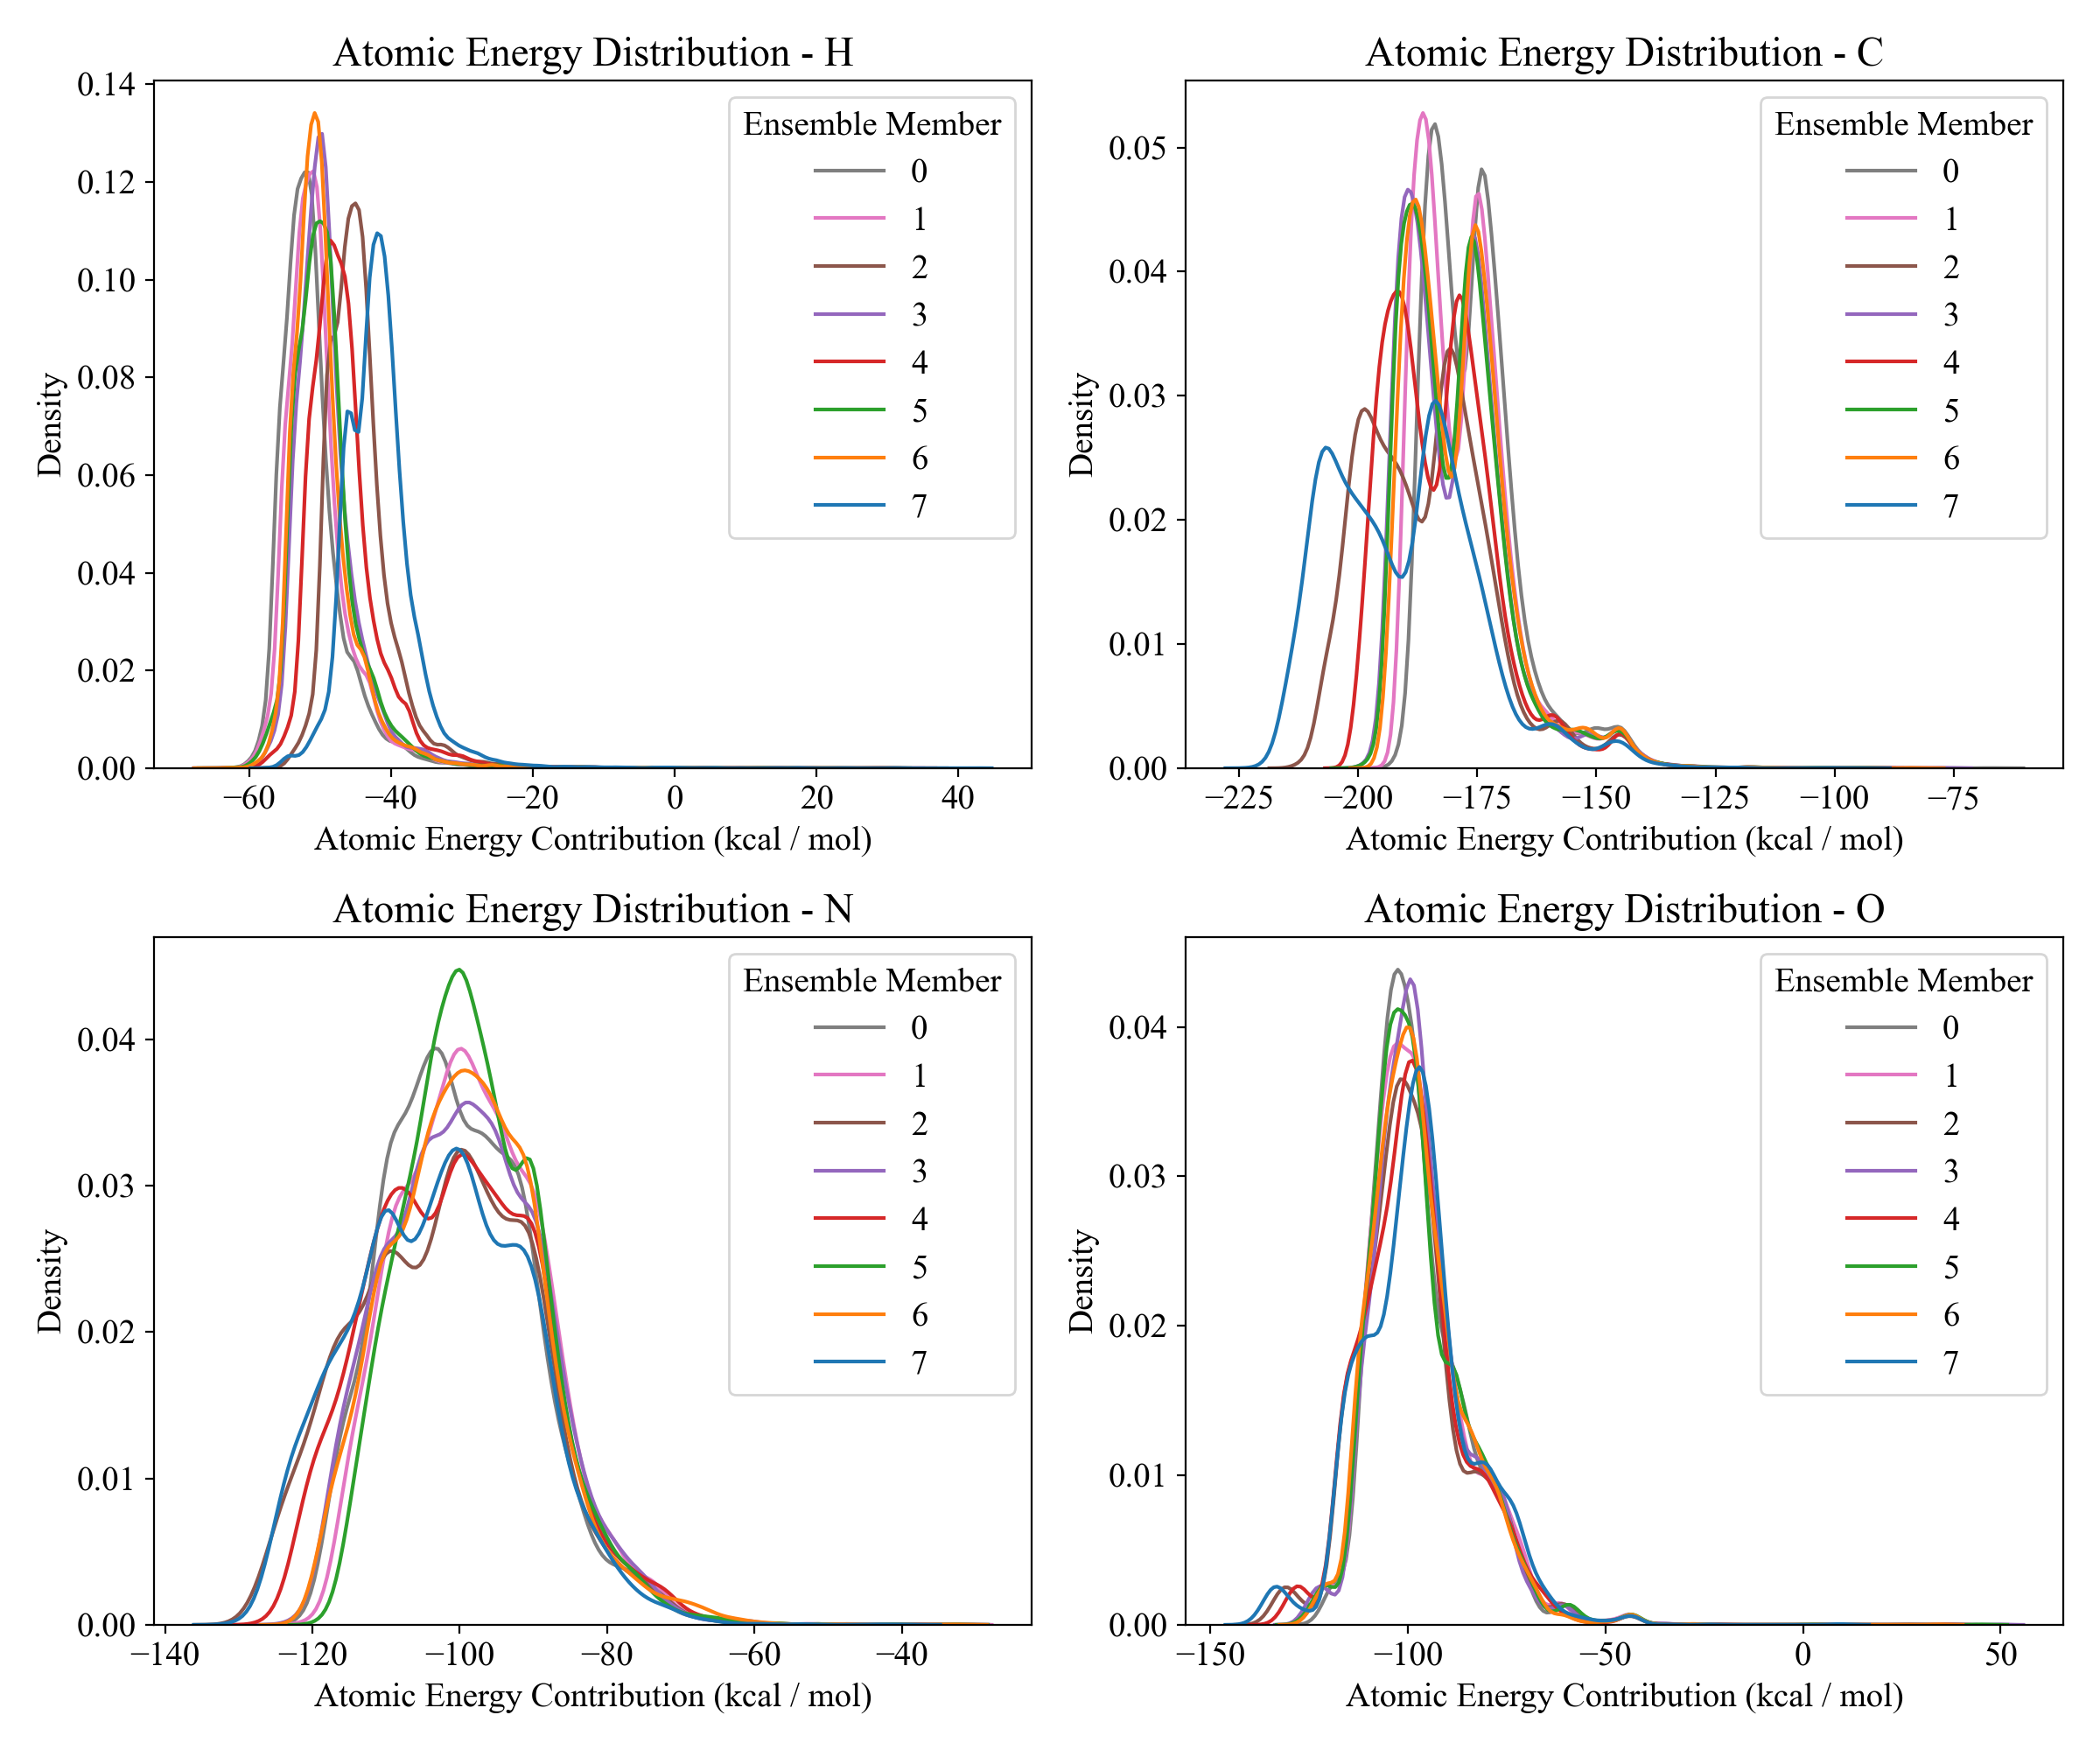
\includegraphics[width=1\linewidth]{Images/2xr_outputs/2xr_1x-first_ae-per-model.png}
    \caption[Atomic energies predicted by ANI-2xr]{Distribution of atomic energy contributions by atom type for the ANI-2xr potential. Values shown in kcal/mol for CHNO atom types on the 1x-first subset.}
    \label{fig:2xr_ae_per_model}
\end{figure}

The difference in the shapes of these distributions is an important aspect of analyzing the predictive uncertainty of ANI neural network potentials.
Due to the differences in hyperparameters used in training, such as the removal of biases, the use of the GELU activation function \cite{gelu} continuous second derivatives improving the smoothness of predicted potential energy surfaces, and the addition of ground state atomic energies and a repulsive term, ANI-2xr will be used to explore trends in uncertainty in predictions by ANI neural networks. 

\subsection{Uncertainty in ANI Neural Network Potentials}
\label{subsec:ANI_uncertainty}

ANI potential models use an ensemble of eight independently models, allowing for the estimation of predictive uncertainty.
This uncertainty metric is frequently used in active learning strategies to guide data selection for model improvement.
Predictive uncertainty has been measured in published models using $\hat{\rho}$; the value 0.23 kcal/mol was empirically chosen for sampling structures with high-error energy predictions via query by committee (QBC) in the active learning process \cite{ani-1x}.
The QBC value, given in Eqn. \ref{eq:energy_qbc}, can be thought of as a binary classifier: molecules with QBC values above 0.23 kcal/mol are highly-uncertain predictions and shouldn't be trusted, while values below 0.23 kcal/mol are trustworthy, agreed upon values by the ensemble.

\begin{equation}
\rho = \frac{\sigma_{E_{\text{Total}}}}{\sqrt{N_{\text{atoms}}}}
\label{eq:energy_qbc}
\end{equation}

This normalization accounts for the size of the molecule, ensuring that uncertainty values remain comparable across different molecular systems. 
In the development of ANI-1x, a threshold value of 0.23 kcal/mol was empirically chosen as the criterion for selecting molecules with high-energy uncertainty for further active learning \cite{ani-1x}.
However, while QBC serves as a useful uncertainty metric for guiding active learning, it introduces a size-dependent limitation. Because $\sqrt{N_\text{atoms}}$ appears in the denominator, molecules with a large number of atoms can exhibit low uncertainty values, even if individual atomic energy predictions are highly uncertain. 
This means that large structures may be misclassified as “low-error” molecules despite containing regions of high uncertainty in their atomic energy contributions. 
Consequently, high-error structures may slip through the active learning process, leading to gaps in the training data for larger molecules.

To explore this issue further, atomic energy predictions can be examined on a per-atom-type basis. 
Figure \ref{fig:2xr_comp6v1_mean-ae-per-atomtype} presents the distribution of mean atomic energy predictions using the ANI-2xr model on the COMP6v1 benchmark set. 
This per-atom decomposition allows for a finer-grained analysis of uncertainty, revealing how specific atomic environments contribute to total energy predictions and where potential weaknesses in the model may arise.

\begin{figure}[H]
    \centering
    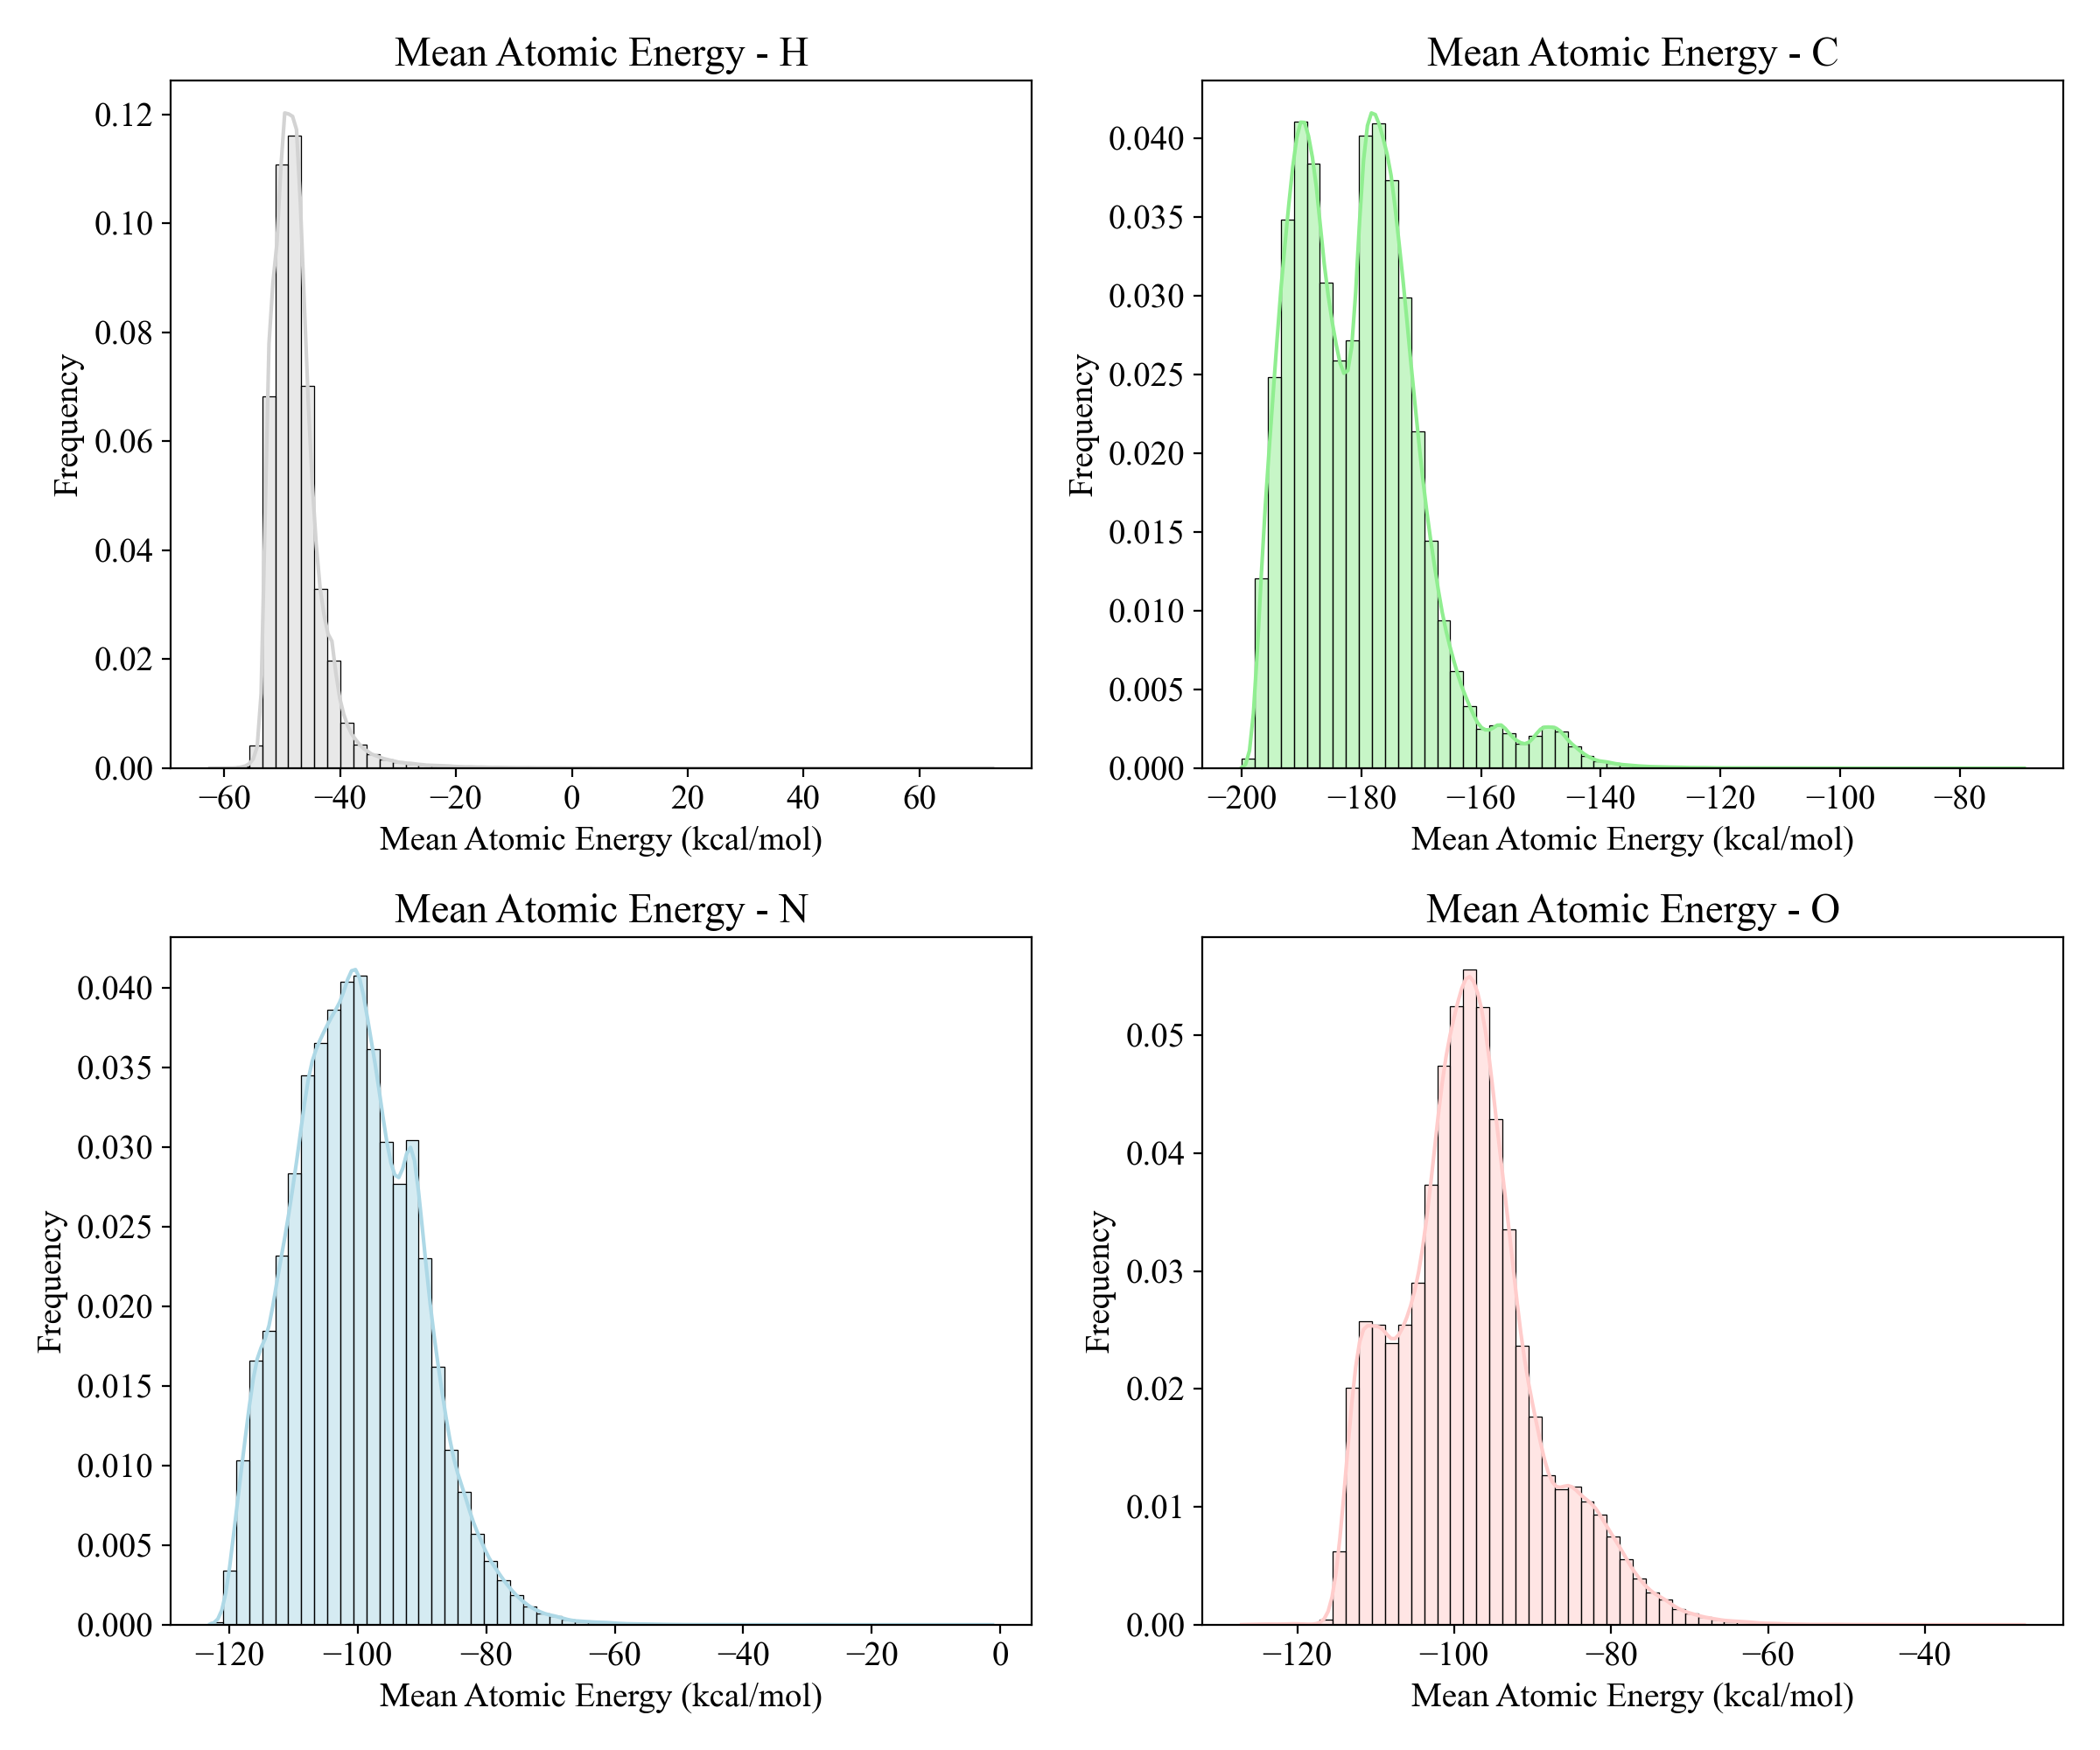
\includegraphics[width=1\linewidth]{Images/2xr_outputs/2xr_comp6v1_mean-ae-per-atomtype.png}
    \caption[Mean atomic energy prediction per-atom with ANI-2xr]{Distribution of predicted mean atomic energies using the ANI-2xr model on the COMP6v1 benchmark set.}
    \label{fig:2xr_comp6v1_mean-ae-per-atomtype}
\end{figure}

By analyzing per-atom energy contributions, it becomes possible to refine uncertainty quantification methods beyond QBC, addressing the size-dependent bias and improving the selection of high-error molecules for retraining in future ANI models.

\subsection{Exploration of the Flaws in Measuring Uncertainty via Predicted Total Energy}
\label{subsec:flaws_in_qbc}

A clear example of size dependence in ANI uncertainty estimation can be illustrated by considering a small molecule with a high query-by-committee (QBC) value. Suppose we start with a simple molecule, such as propane (C\textsubscript{3}H\textsubscript{8}), where a particular atomic region exhibits a relatively high uncertainty in its predicted atomic energies. Because QBC normalizes by the square root of the number of atoms $\left(\sqrt{N_\text{atoms}} \right)$, the uncertainty estimate is influenced heavily by molecular size.

Now, consider a structurally similar but larger molecule, \authorRemark{REWRITE THIS TO THE m-epoxide EXAMPLE ... } such as undecane (C\textsubscript{11}H\textsubscript{24}), which is derived from propane by extending one of its methyl functional groups into a 10-carbon chain. Despite this significant increase in molecular size, the region of high atomic uncertainty in the original molecule still exists—for example, in the same local chemical environment near the initial site of uncertainty. However, because $\left(\sqrt{N_\text{atoms}} \right)$ is much larger, the total molecular uncertainty value ($\rho$) is now lower, even though the model's uncertainty in that specific region has not improved.

This example demonstrates how large molecules can exhibit deceptively low QBC values, making it more difficult to identify high-error structures in active learning. As a result, potentially problematic regions of uncertainty can be overlooked in training set refinement, leading to overconfidence in predictions for large systems. Such effects highlight the need for alternative uncertainty quantification methods that account for localized atomic errors rather than relying solely on global molecular uncertainty metrics.

As the energy of molecules is predicted as a sum of atomic contributions---and therefore, one could say, the networks are actually predicting atomic energies---the first exploration into an atomistic uncertainty method was into the atomic energy contribution predicted for each atom.

\section{Uncertainty of Atomic Energy Predictions}
\label{sec:uncertainty_atomic_energies}

Predictive uncertainty in ANI neural network potentials extends beyond total molecular energy predictions, affecting atomic energy contributions on a per-atom basis. The standard deviation in atomic energy predictions across an ensemble of ANI models provides insight into how confidently the model assigns energetic contributions to individual atoms. Figure \ref{fig:2xr_comp6v1_stdev-ae-per-atomtype} illustrates the distribution of atomic energy standard deviations for different atom types (H, C, N, O) using the ANI-2x model on the COMP6v1 benchmark set. Higher uncertainty in atomic energy predictions often correlates with underrepresented chemical environments in the training data, where the model struggles to generalize beyond learned patterns. Additionally, atoms in highly strained or reactive regions tend to exhibit greater variance, reflecting the challenge of accurately capturing energy contributions in chemically complex systems.

\begin{figure}[H]
    \centering
    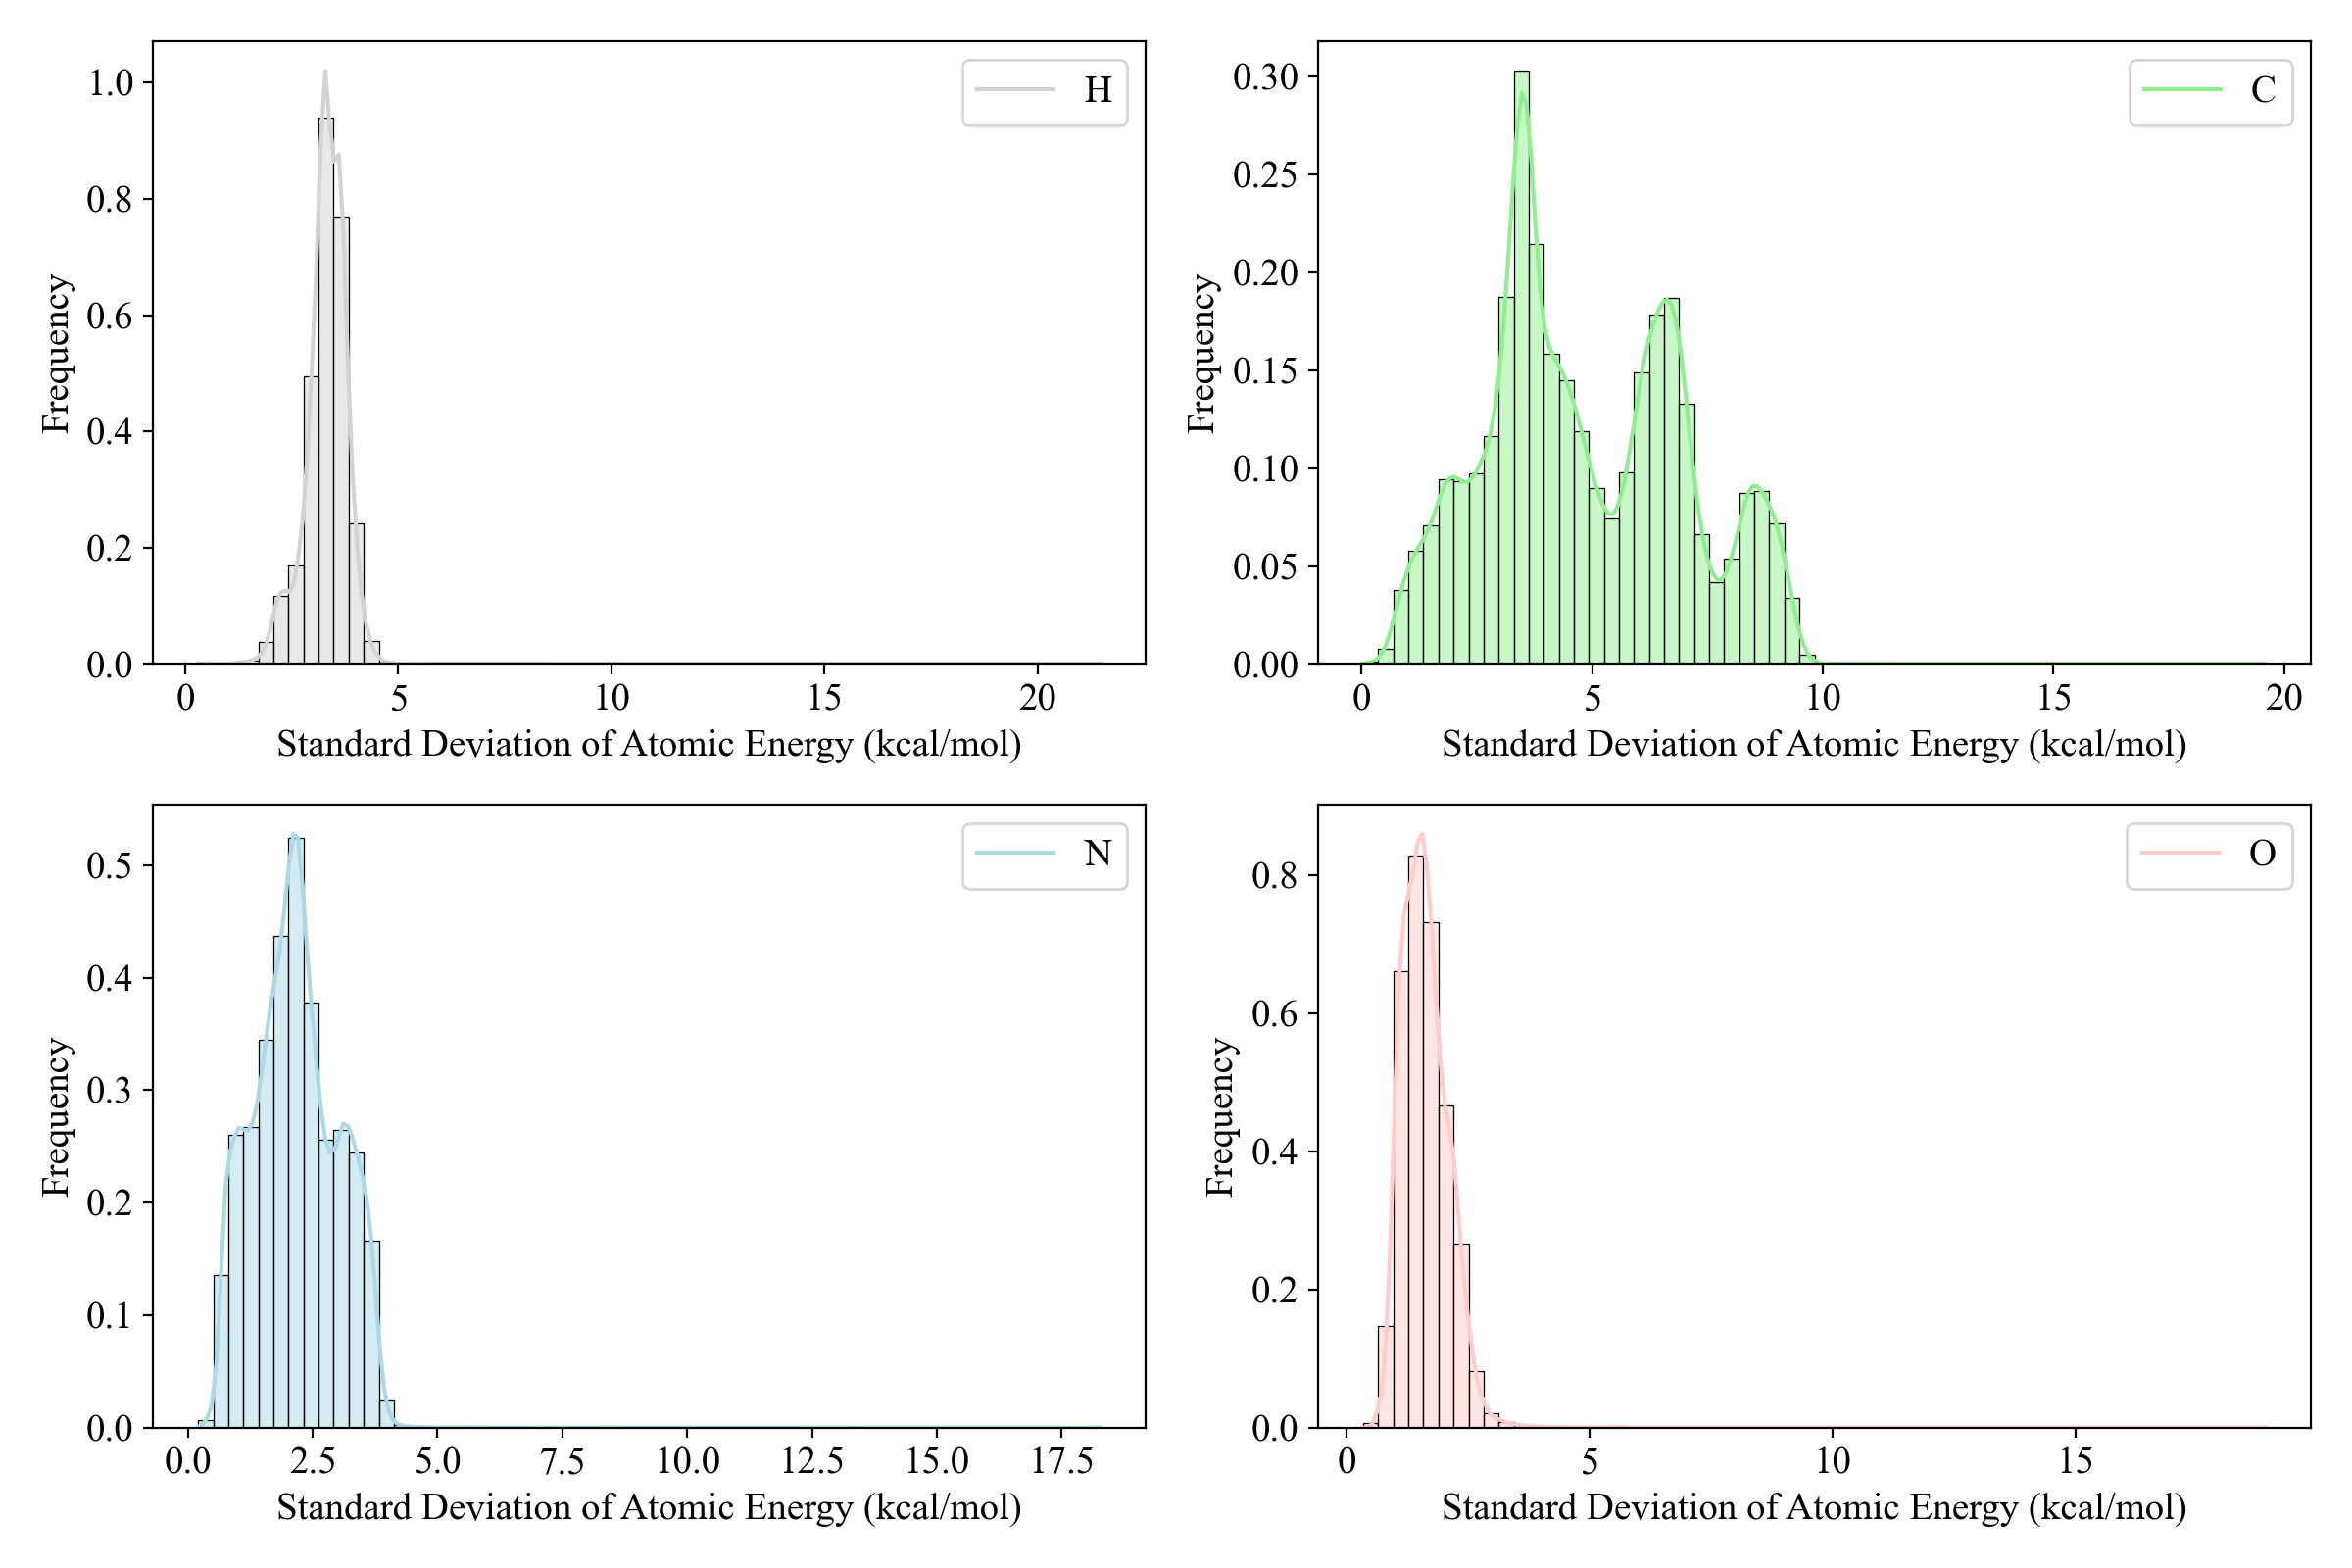
\includegraphics[width=1\linewidth]{Images/2xr_outputs/2xr_comp6v1_stdev-ae-per-atomtype.png}
    \caption[Standard deviation in predicted atomic energy contribution for H, C, N, O atom types]{Distribution of standard deviation in predicted atomic energies using the ANI-2x model on the COMP6v1 benchmark set.}
    \label{fig:2xr_comp6v1_stdev-ae-per-atomtype}
\end{figure}

Higher uncertainty in atomic energy contributions often arises in chemically complex or underrepresented environments in the training data. While carbon and oxygen atoms typically exhibit lower variance due to their frequent occurrence in organic molecules, hydrogen atoms display a broader spread, reflecting their dependence on local bonding environments. This is particularly relevant in systems where heteroatoms or extended conjugation patterns influence local electronic structure, leading to higher variability in atomic energy assignments.
An illustrative example of this phenomenon can be seen in methane (CH\textsubscript{4}), which is a highly symmetric molecule with four chemically equivalent hydrogen atoms and a single carbon center. Figure \ref{fig:ch4_stdev_ae} presents the standard deviation in atomic energy contributions for CH\textsubscript{4} across the ANI-2xr model ensemble, compared to the total energy uncertainty distribution in the 1x-first test set.

\begin{flushleft}
\begin{multiFigure}
    \addFigure{0.31}{Images/ch4.png}
    \addFigure{0.68}{Images/ch4_example/ch4_2xr_total-e-qbc.png} \\
    \addFigure{1}{Images/ch4_example/ch4_2xr_stdev-ae.png}
\captionof{figure}[CH\textsubscript{4} atomic energy distribution vs 1x-first]{
(A) Structure of geometry-optimized CH\textsubscript{4}; 
(B) Plot of the distribution of total energy QBC across the 1x-first test set, 
(C) standard deviation in predicted atomic energy for hydrogen (left) and carbon (right); 
the red lines show the standard deviation in CH\textsubscript{4} total energy (B) and atomic energy contributions (C).
}
\label{fig:ch4_stdev_ae}
\end{multiFigure}
\end{flushleft}

While total molecular energy predictions for CH\textsubscript{4} remain relatively low in uncertainty, the per-atom standard deviations reveal higher variability in atomic energy contributions, particularly in hydrogen. This suggests that even in highly symmetric molecules, ANI's per-atom energy assignments may be non-trivial, introducing potential sources of error in energy decomposition analyses.

The per-atom uncertainty in ANI models is not only influenced by the training data but also by learned covariances across network predictions. The atomic energy contributions predicted by different models within the ANI ensemble exhibit correlated variations, where changes in one atomic energy may be systematically offset by adjustments in another.
For example, Table \ref{tbl:ch4_AEs} reports the atomic energy contributions predicted by each model in the ANI-2xr ensemble for CH\textsubscript{4}. While the individual atomic energies fluctuate across models, the sum of atomic energies remains tightly constrained, with a standard deviation an order of magnitude lower than that of the individual atomic contributions.

% Tables suck, but this helped me align columns and headers separately:
\begin{table}[hbt]
\centering
\caption[CH\textsubscript{4} atomic energy contributions per-model]{
Atomic energy contributions by atom type in a geometry-optimized molecule of CH\textsubscript{4}, with four equivalent hydrogen atoms. 
Additionally, the sum over all atoms, and that sum after passing through the TorchANI EnergyShifter. 
Values obtained from an ensemble of ANI models (ANI2xr); the last column shows the standard deviation of predictions across the ensemble. 
All values are in kcal/mol.
}\label{tbl:ch4_AEs}
    \begin{tabularx}{\textwidth}{%
    >{\raggedleft\arraybackslash}r  % Numeric
    >{\raggedleft\arraybackslash}r  % Numeric
    >{\raggedleft\arraybackslash}r  % Numeric
    >{\raggedleft\arraybackslash}r  % Numeric
    >{\raggedleft\arraybackslash}r  % Numeric
    }  
\hline
Model & Carbon & Hydrogen  & Sum of atomic energies & Molecular energy \\
\hline
Mean prediction & -199.0069 & -55.1013 & -419.4123 & -25413.8125 \\
1 & -219.4329 &  -50.0170 &  -419.5012 &  -25413.9043 \\
2 & -194.7117 &  -56.1991 &  -419.5081 &  -25413.9102 \\
3 & -192.8823 &  -56.6466 &  -419.4689 &  -25413.8691 \\
4 & -201.5683 &  -54.4451 &  -419.3490 &  -25413.7500 \\
5 & -196.5227 &  -55.7060 &  -419.3471 &  -25413.7500 \\
6 & -212.9323 &  -51.5945 &  -419.3103 &  -25413.7109 \\
7 & -186.5623 &  -58.2018 &  -419.3694 &  -25413.7715 \\
8 & -187.4427 &  -58.0003 &  -419.4441 &  -25413.8457 \\
Standard deviation &  11.7621 &  2.9412 &  0.0775 &  0.0775 \\
\hline
\end{tabularx}
\end{table}

This covariance, defined in Eqn. \ref{eq:covariance}, reflects a learned compensation mechanism where certain atomic energy predictions systematically adjust in response to others.

\begin{equation}
    \label{eq:covariance}
    \text{cov}(x, y) = \mathbb{E}[(x - \mathbb{E}[x])(y - \mathbb{E}[y])]
\end{equation}

This suggests that ANI models learn relative atomic energy distributions, where variations in one atom's contribution are counterbalanced by adjustments in others to maintain a stable total molecular energy. To better understand this effect, Figure \ref{fig:ch4_covariance} presents covariance matrices of atomic energy contributions for CH\textsubscript{4} and pentane (C\textsubscript{5}H\textsubscript{12}), highlighting correlation patterns between atomic contributions in molecules of different sizes.

\begin{flushleft}
\begin{multiFigure}
    \addFigure{0.2}{Images/covariance/ch4_labeled.png}
    \addFigure{0.65}{Images/covariance/ch4_covariance.png}
    \addFigure{0.28}{Images/covariance/c5h12_labeled}
    \addFigure{0.65}{Images/covariance/c5h12_covariance.png} \\
\captionof{figure}[Atomic energy covariance matrices]{
(A) Geometry-optimized structure of CH\textsubscript{4}; 
(B) Matrix visualizing the covariance of atomic energies predicted by ANI-2xr for this structure of CH\textsubscript{4}; 
(C) Structure of geometry-optimized C\textsubscript{5}H\textsubscript{12}; 
(D) Covariance matrix for predicted atomic energies of C\textsubscript{5}H\textsubscript{12}.}
\label{fig:ch4_covariance}
\end{multiFigure}
\end{flushleft}

This compensatory behavior suggests that ANI models do not learn absolute atomic energies in isolation, but rather relative energy distributions that maintain a consistent total molecular energy. As a result, variations in one atomic contribution are often counterbalanced by adjustments in neighboring atoms, preserving overall energetic stability while allowing individual atomic predictions to fluctuate.
These covariance effects contribute to the observed size dependence in ANI model uncertainty, where molecular energy predictions remain stable while per-atom uncertainties fluctuate.
This behavior is due to learned covariances across networks, where, for example, carbon atomic energies learn to offset hydrogen energy contributions in the training process. This relationship is defined in Eqn. \ref{eq:total_e_covariance}.

\begin{equation}
    \sigma_{E_{\text{total}}}^2 = \sum_i^{N \text{ (atoms)}} \sigma_{E_{\text{atomic}}}^2 + 2 \sum_i^N \sum_{j \neq i}^N \text{cov}(x_i, y_j) = \sum_{i,j}^N \text{cov}(x_i, x_j)
    \label{eq:total_e_covariance}
\end{equation}

This covariance-driven redistribution of uncertainty is a key challenge in using ANI for uncertainty-aware simulations, as it impacts force predictions, molecular dynamics stability, and error estimation in out-of-sample predictions.

\section{Need for a Practical, Physical Quantity to Estimate Uncertainty}
\label{sec:practical_physical_quantity_for_uncertainty}

The predictive uncertainty in ANI models has primarily been examined through atomic energy distributions, but these values lack intrinsic physical meaning beyond their role in reproducing the total molecular energy. A fundamental limitation of atomic energy assignments is their model dependence—each of the eight neural networks in the ensemble learns a slightly different decomposition of molecular energy, leading to inconsistencies in per-atom contributions. This variability makes atomic energies ill-suited as a reliable uncertainty measure, as they do not correspond to an independently verifiable physical property.

A more robust alternative lies in atomic forces, which ANI models also predict as derivatives of the potential energy surface, shown in Equation \ref{eq:force_dE}. 
\begin{equation}
    \vec{F} = -\nabla E
    \label{eq:force_dE}
\end{equation}

Unlike atomic energies, forces directly correspond to the physical structure and motion of molecules, as they describe how atoms interact under the influence of a potential. Forces dictate molecular geometry, vibrational frequencies, reaction pathways, and dynamics, making them a natural choice for evaluating model reliability. Since ANI is trained to approximate the true quantum mechanical PES, its force predictions serve as an indirect measure of how well the model captures the curvature of the PES, providing insight into both local stability and model confidence.

The combined energy and force loss function used in ANI training, given in Eqn. \ref{eq:force_loss}, minimizes the molecular energy error while also penalizing discrepancies in predicted atomic forces. This introduces an additional constraint that enhances the physical reliability of the learned potential energy surface:

\begin{equation}
\mathcal{L}_{\text{E \& }\vec{\text{F}}} = 
\frac{1}{N_{\text{M}}} 
\sum_{i=1}^{N_\text{M}} 
\left[ \left( \frac{
\left( E_{\text{ANI}}^{\text{o},i} - E_{\text{QM}}^{\text{o},i} \right)^2}
{\sqrt{N_{\text{atoms}}}} \right)
+ 0.1 \ast \left( 
\frac{\sum_{j=1}^{N_{\text{atoms}}} 
\left( \vec{f}_{\text{ANI}}^{j} - \vec{f}_{\text{QM}}^{j}\right)^2}{N_{\text{atoms}}} 
\right) \right]
\label{eq:force_loss}
\end{equation}

This loss function consists of two key components that work together to optimize both molecular energy and atomic force predictions. The first component addresses energy loss by computing the mean squared error (MSE) between the predicted molecular energy and the reference quantum mechanical energy. To ensure that large molecules do not disproportionately influence the optimization process, the loss is normalized by the square root of the number of atoms in the system. This normalization maintains consistency in model performance across different molecular sizes. The second component focuses on force loss, which is calculated as the difference between the predicted atomic forces and the quantum mechanical reference forces. Since each atom experiences forces that determine molecular motion and stability, the force loss is averaged over all atoms in the molecule, treating each force vector as an independent target for training. To balance the contributions of energy and force errors, a scaling factor of 0.1 is introduced, preventing one component from dominating the learning process. This ensures that the model refines both energy and force predictions simultaneously, leading to a more physically meaningful representation of molecular interactions.

By training ANI to predict forces along with energies, we gain access to a physically meaningful metric for uncertainty estimation. Since forces describe how gradients of the potential energy surface vary across atomic positions, their accuracy directly reflects the model's ability to approximate quantum mechanical interactions.
When an ANI model encounters a molecule outside of its training distribution, its force predictions may become erratic or inconsistent across the ensemble, reflecting the model’s lack of confidence in extrapolating beyond familiar chemical environments. By analyzing the standard deviation in force predictions across the ANI ensemble, we can construct a size-independent measure of uncertainty that is directly tied to physical observables rather than arbitrary atomic energy assignments.
This insight forms the foundation for the next chapter, where we explore how force-based uncertainty metrics can be used to assess ANI model reliability in molecular simulations, and how these methods compare to traditional QBC-based energy uncertainty approaches.%
\chapter{Uncertainty in atomic force predictions}
\label{chapter3}

The reliability of machine-learned interatomic potentials depends not only on the accuracy of reproducing reference quantum mechanical data but also on the ability of such models to quantify uncertainty in predictions, as the desired applications of such ML models are for (large) systems that ground-truth data is inaccessible due to prohibitive scaling and the limits of computational efficiency.
Ensemble-based methods, such as ANI models, offer an empirical approach to assessing predictive confidence; however, a robust, universally applicable, and physically meaningful uncertainty measure for atoms of different species remains a challenge.
In the broader field of deep learning, uncertainty quantification has been explored through various strategies, including ensemble averaging \cite{optimal_ensemble_averaging_naftaly, ensemble_deep_learning_review_ganaie}, scalable uncertainty estimation methods \cite{scalable_uncertainty_scalia, scalable_uncertainty_lakshminarayanan}, and dropout-based implementations \cite{dropout1, dropout2, uncertainty_quantification_dropout_wen} to improve predictive capabilities by temporarily removing nodes from the input and hidden layers. 

These approaches aim to distinguish between epistemic uncertainty, which arises from model limitations and can be reduced with additional training data, and aleatoric uncertainty, which reflects inherent noise in the data itself. 
In atomistic simulations, these principles suggest that uncertainty estimation must capture both model limitations and physical constraints imposed by molecular interactions \cite{uncertainty_atomistic_ml_peterson}.
Within the domain of neural network potentials, ensembles have been widely used to quantify predictive confidence, offering a direct measure of variance in model outputs \cite{uncertainty_of_nnp_ensembles_kahle}. 
However, most existing uncertainty estimation techniques focus on energy predictions, rather than on the fundamental physical quantities that dictate molecular behavior. 
Since forces define the curvature of the potential energy surface, an uncertainty measure derived from force predictions would provide deeper insight into model reliability and transferability.

This chapter explores uncertainty estimation in ANI models without altering the already well-performing neural network model architecture. 
We seek an explainable \cite{uncertainty_quantification_yang} uncertainty quantification metric to determine whether force-based uncertainty offers a more practical and scalable alternative to traditional energy-based uncertainty measures.


\section{Potential Solution}
\label{sec:uncertainty_potential_solution}

In the search for a reliable atomistic metric to estimate uncertainty in molecular energy predictions, we face a fundamental challenge: the true energy of a system is unknown during inference, making direct error quantification impossible. 
Instead, we require a proxy quantity, one that can be predicted by the network and used as an internal measure of confidence without explicit reference to a ground truth.
Atomic energies, while conceptually appealing, proved unsuitable for this purpose; due to the model-dependent energy decomposition, different networks in the ANI ensemble learn distinct atomic energy contributions, leading to inconsistent assignments across models.
Attempts to reduce the uncertainty in predicted atomic energies in a purely data-driven ML model inevitably compromises the accuracy of the total molecular energy prediction.

For an uncertainty measure to be viable, it must be supported by fundamental physical principles and computed in an explainable manner within the existing neural network framework. 
Unlike atomic energies, forces are directly governed by quantum mechanical principles, as they correspond to the gradient of the potential energy surface with respect to atomic coordinates (Eqn. \ref{eq:force_dE}). 
Because every atom in a molecular system experiences forces, this quantity is universally defined---except in the case of a true global minimum, which is inconsequential for MD applications---offering a more consistent target for uncertainty estimation.

A considered alternative approach could involve using dipole moments as an uncertainty metric, given their sensitivity to electronic structure and molecular geometry.
However, dipoles present two key limitations: they do not exist for certain molecular systems, such as nonpolar molecules, and they are global properties, meaning they do not offer localized atomic-level uncertainty estimates.
In contrast, atomic forces remain well-defined even in near-equilibrium geometries, with only minor fluctuations in magnitude depending on molecular stability.

Since molecular dynamics simulations almost exclusively explore non-equilibrium conformations, the forces acting on atoms are virtually always nonzero, reinforcing their utility as a generalizable measure of model confidence.
Even in the case of global equilibrium, models should be tuned to agree on atomic forces predicted to be equal to zero. 
Thus, forces present a promising avenue for quantifying predictive uncertainty at the atomistic level and can be used to explore whether the variability in these values provides a meaningful, physically grounded measure of model reliability.


\subsection{Forces}
\label{subsec:forces}

Atomic forces provide a direct means of assessing the landscape of the potential energy surface (PES), making them a natural candidate for evaluating uncertainty in ANI predictions. 
Since forces correspond to the gradient of energy with respect to atomic positions, they encode local curvature information that is critical for modeling molecular behavior, including geometry optimizations, vibrational properties, and molecular dynamics simulations. 
Unlike atomic energy decompositions, which lack a strict physical interpretation, atomic forces are observable, well-defined, and physically meaningful across all molecular systems.

Forces act on individual atoms and directly govern how they respond to their immediate chemical environment. This atom-wise resolution makes forces particularly valuable for assessing model performance at a finer scale, where uncertainty can be linked to specific atomic interactions rather than a global molecular quantity. 
Because forces inherently reflect the steepness and shape of the potential energy surface, they provide insight into how well the model captures subtle variations in bonding, steric effects, and reaction coordinates---critical aspects that define the accuracy of interatomic potentials.

The first approach taken in assessing model agreement in predicted forces was to compute the cosine similarity of the force vector predicted, for each atom, by each model in the ensemble. This relationship is given in Equation \ref{eq:cosine_similarity}.

\begin{equation}
\text{cosine similarity} = \frac{\vec{f_1} \cdot \vec{f_2}}{\max(\|\vec{f_1}\|_2 \cdot \|\vec{f_2}\|_2, \epsilon)}
\label{eq:cosine_similarity}
\end{equation}

Here, two force vectors, $\vec{f_1}$ and $\vec{f_2}$, which point in exactly the same direction would have a cosine similarity of 1, orthogonal vectors would have a value of 0, and anti-parallel vectors would have a similarity value of -1.
The parameter $\epsilon$ is a small number ($10^{-8}$) to prevent the possibility of division by zero. 
Figure \ref{fig:2d_2xr_comp6v1-forces-cos_sim} presents a per-model cosine similarity analysis of atomic force predictions from COMP6V1 benchmark dataset across the ANI-2xr ensemble compared to reference DFT forces. 

\begin{figure}[H]
    \centering
    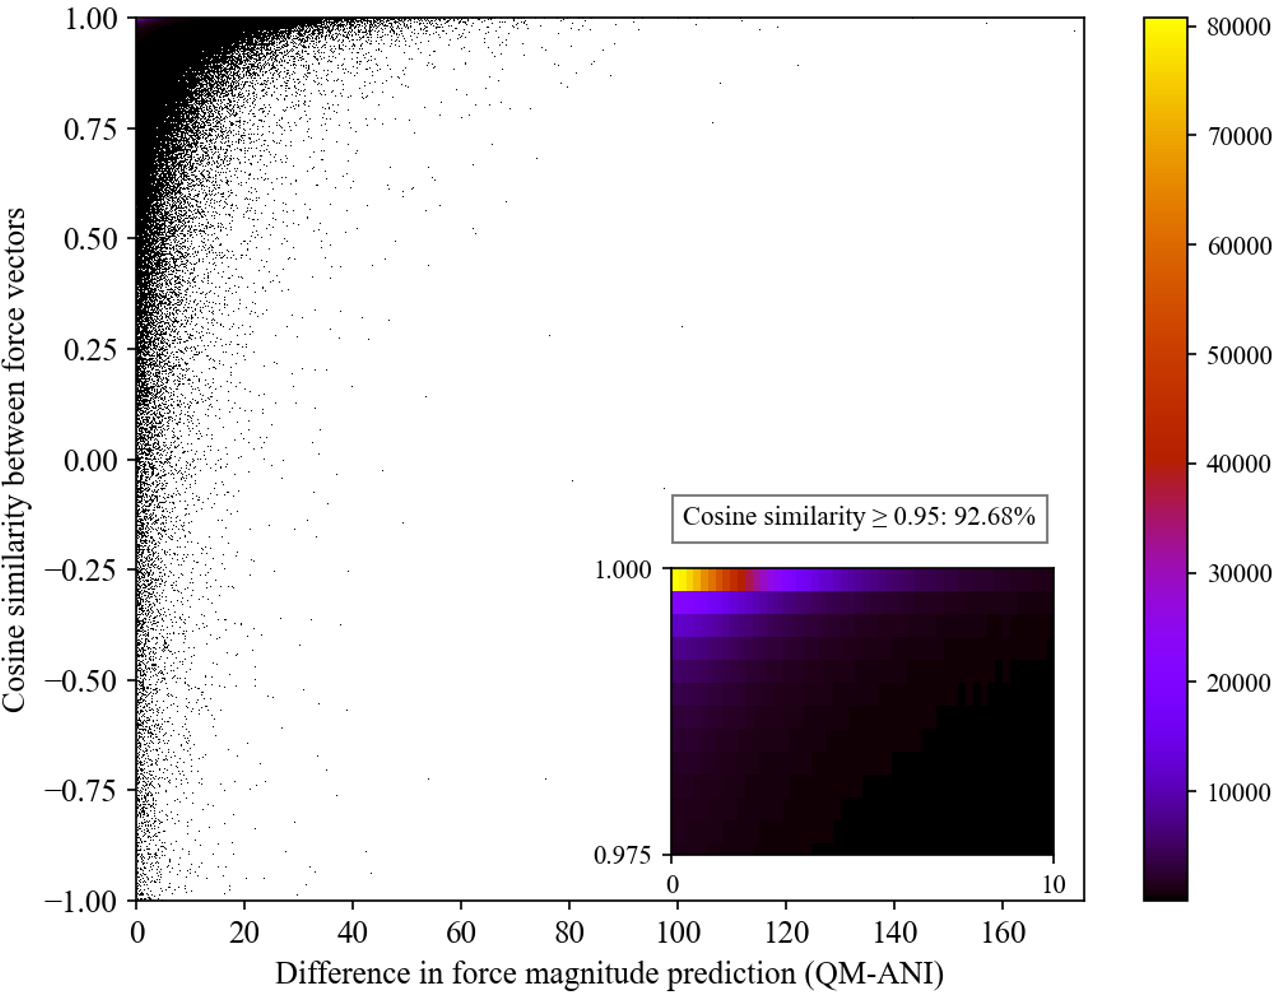
\includegraphics[width=1\linewidth]{Images/2xr_forces/cos_sim-hist2d-insert.png}
    \caption[2D histogram of cosine similarity measure of predicted atomic force vectors]{ \authorRemark{Give these different captions} \\
    Cosine similarity between ANI predicted forces (per-model) versus the DFT reference forces on the COMP6v1 benchmark dataset.
    }
    \label{fig:2d_2xr_comp6v1-forces-cos_sim}
\end{figure}

This metric captures the directional agreement between predicted and true force vectors, illustrating that ANI models, in nearly all cases, predict forces that align closely with the correct direction on the PES. 
Even in cases where predictions deviate, these errors tend to occur in low-error structures near equilibrium, where the magnitude of the force vector is very small. 
This suggests that while absolute force magnitudes vary across the ensemble, the network reliably captures the qualitative features of the PES.
The cosine similarity data is re-plotted in three dimensions in Figure \ref{fig:2xr_comp6v1-forces-cos_sim}, further demonstrating the directional agreement of predicted atomic forces.

\begin{figure}[H]
    \centering
    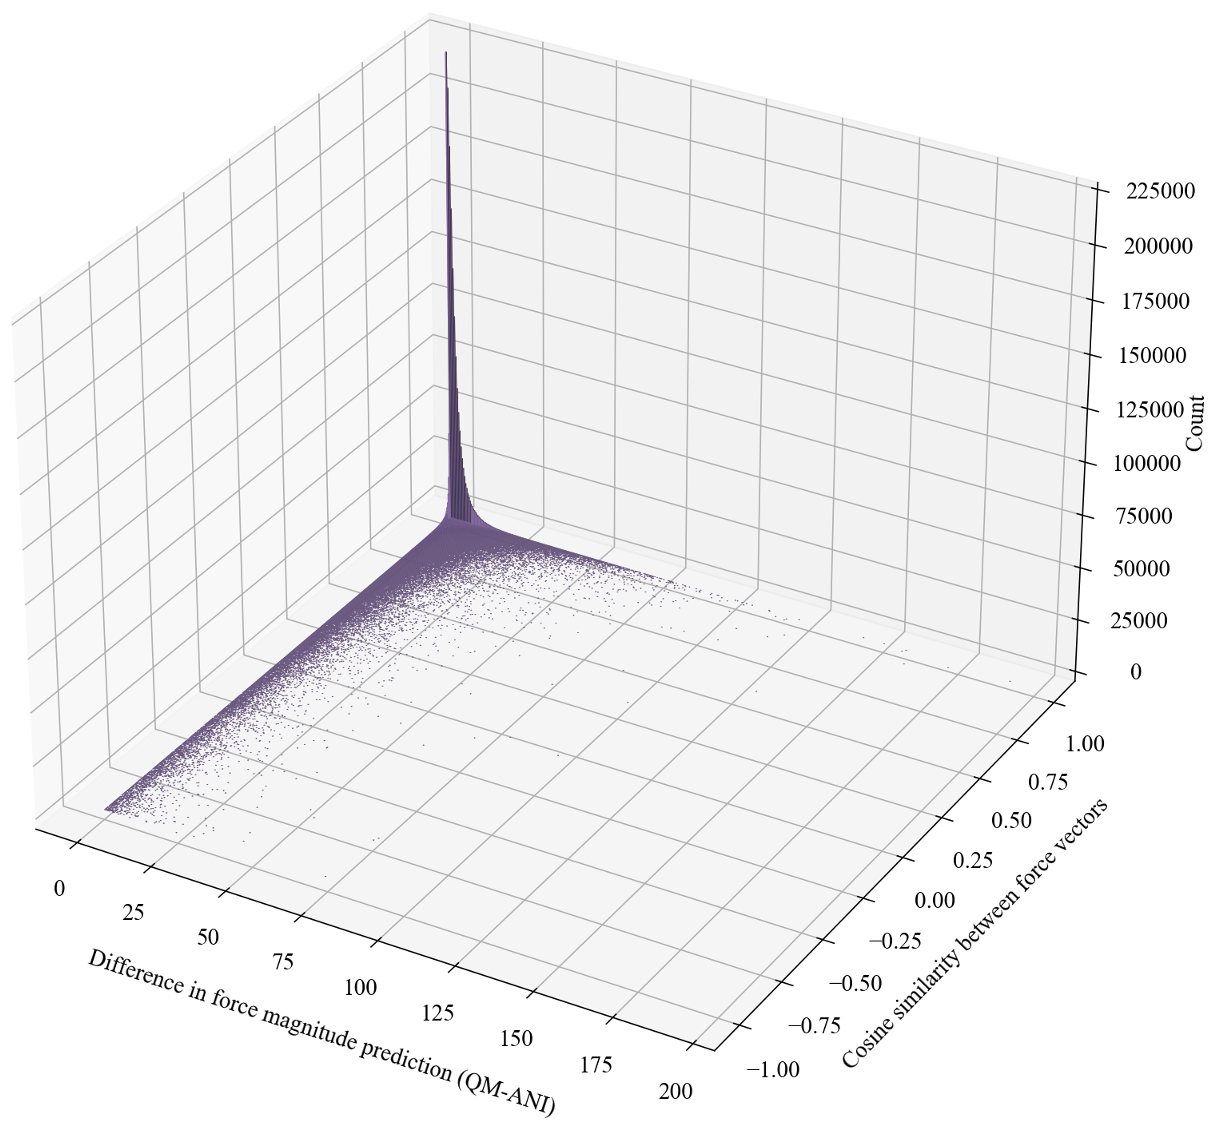
\includegraphics[width=1\linewidth]{Images/2xr_forces/2xr_comp6v1_force-cosine_sim-bar3d.png}
    \caption[3D histogram of cosine similarity measure of predicted atomic force vectors]{
    Cosine similarity between ANI predicted forces (per-model) versus the DFT reference forces on the COMP6v1 benchmark dataset.
    }
    \label{fig:2xr_comp6v1-forces-cos_sim}
\end{figure}

One of the key advantages of using force predictions for uncertainty quantification is their sensitivity to local errors in the PES. 
Atomic forces provide spatially resolved information that reflects the stability of individual atoms within their local chemical environment. 
This enables a more granular assessment of uncertainty, where high-uncertainty atoms may indicate regions of the molecule that are poorly represented in the training data. 
Additionally, because forces influence molecular motion in dynamics, uncertainty in force predictions may translate directly to instabilities in simulations, making it important to assess their reliability in MD applications.

Another consideration is the role of ensemble-based predictions in force uncertainty estimation. In ANI, force vectors are obtained independently from each model within the ensemble, meaning that variations in force predictions across the ensemble provide a direct measure of model disagreement. This disagreement can be leveraged as an uncertainty metric, where a high standard deviation in force predictions signals regions of chemical space where the model lacks confidence. Importantly, unlike atomic energies, which exhibit compensatory behavior across the ensemble (as discussed in Section \ref{sec:uncertainty_atomic_energies}), force predictions do not sum to a fixed total value. This means that force uncertainty is not artificially constrained, making it a more reliable measure of true model uncertainty rather than an artifact of network training.

Beyond uncertainty quantification, force predictions also offer practical advantages for improving the robustness of ANI models. Since forces define the shape and curvature of the PES, incorporating force-based uncertainty into active learning strategies could enhance the selection of training data, ensuring that new data points are sampled in regions of highest uncertainty. This approach has been explored in other uncertainty-aware machine learning models \cite{uncertainty_atomistic_ml_peterson}, but its application to force-driven active learning in ANI remains an open area of research.

In summary, atomic forces provide a compelling alternative to atomic energy-based uncertainty measures, offering physically meaningful, localized, and dynamically relevant information about model reliability. The strong directional agreement between ANI-predicted and reference forces demonstrates that, even in cases of mild uncertainty, the model remains faithful to the underlying physics of molecular interactions. The following sections will further explore the statistical properties of force predictions and investigate how ensemble variance can be used as a practical uncertainty metric in molecular simulations.

While atomic forces present a promising avenue for uncertainty quantification, they also introduce a new challenge: each atom's force prediction consists of three independent vector components, corresponding to the 
$x$,$y$, $z$ directions. Unlike total energy, which is a scalar quantity that can be directly compared across different molecules, force vectors introduce dimensional complexity when attempting to reduce uncertainty to a single measure. A meaningful uncertainty metric must distill this multi-component information into a single scalar value that captures the reliability of force predictions without discarding essential physical details.

Force vectors inherently contain two distinct aspects: direction and magnitude. In the previous analysis, we evaluated force directionality by considering cosine similarity between predicted and reference force vectors. This measure allowed us to assess how well the ANI models capture the qualitative structure of the potential energy surface, ensuring that forces point in the correct directions even when individual model predictions differ. However, directional agreement alone does not provide a complete picture of uncertainty—forces with similar orientations may still differ significantly in magnitude.

To develop a comprehensive force-based uncertainty measure, it is necessary to investigate the second aspect of force predictions: magnitude variations across the ensemble. If models in the ensemble consistently predict similar force magnitudes, we can infer that the model is making confident predictions in that region of chemical space. Conversely, if the ensemble exhibits high variance in force magnitudes, this suggests increased uncertainty, potentially indicating that the model has encountered an unfamiliar molecular environment.

The following sections will focus on force magnitude variability as a key metric for uncertainty estimation. By examining how force magnitudes fluctuate across the ensemble, we aim to construct a single, physically meaningful uncertainty measure that accounts for both the direction and strength of predicted atomic interactions.

\subsection{Force Magnitudes}
\label{subsec:force_magnitudes}

While the previous section demonstrated that ANI models accurately predict the direction of atomic forces, an equally important aspect of force reliability is their magnitude. The magnitude of an atomic force vector determines how strongly an atom is being pulled or pushed within the potential energy surface (PES), making it a crucial factor in molecular dynamics simulations, vibrational analysis, and transition state searches. If a neural network potential (NNP) systematically underestimates or overestimates force magnitudes, it could lead to errors in predicted reaction kinetics, structural stability, or even failures in long-time dynamical simulations.

\begin{figure}[H]
    \centering
    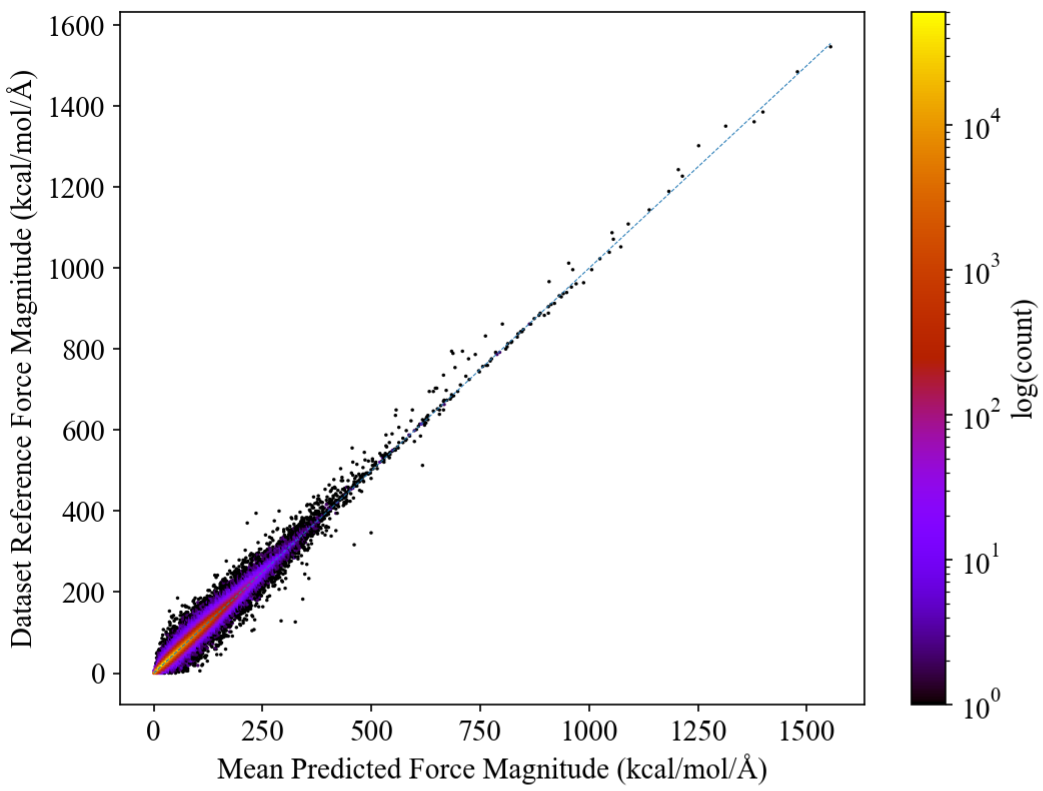
\includegraphics[width=1\linewidth]{Images/2xr_forces/2xr_comp6v1_force-dft-vs-mean_ani.png}
    \caption[Mean predicted atomic force magnitude vs DFT reference]{Predicted force magnitudes vs DFT reference force magnitudes on the COMP6v1 benchmark dataset.}
    \label{fig:2xr_comp6v1-forces-ani_vs_ref}
\end{figure}

Figure \ref{fig:2xr_comp6v1-forces-ani_vs_ref} presents a comparison between the mean force magnitudes predicted by ANI-2x models and the corresponding reference DFT forces. The near-perfect correlation indicates that ANI is not only capable of capturing the qualitative structure of the PES but also reproduces the quantitative force magnitudes with remarkable accuracy. This suggests that ANI models, despite being trained primarily on total energy loss functions, inherently learn force relationships with high precision. The success of ANI in predicting force magnitudes reinforces its applicability for molecular simulations where atomic forces dictate physical behavior, ensuring that molecular geometries evolve realistically under machine-learned potentials.

Given this high level of accuracy, one might initially question whether force magnitudes could serve as an effective uncertainty measure. After all, if ANI reliably reproduces DFT-level force magnitudes, does this not indicate that its uncertainty is already minimized? However, a strong mean prediction does not necessarily preclude fluctuations at an individual atomic or molecular level, particularly across different models in the ensemble. The figure only represents the mean force magnitudes over all molecules in the dataset, without accounting for per-atom variability or systematic differences among individual models. Therefore, while ANI performs well on average, ensemble disagreement may still highlight regions of higher uncertainty, even in cases where the mean force magnitude closely aligns with the DFT reference.

One potential avenue for force-based uncertainty quantification is to examine the variance in predicted force magnitudes across the ensemble. Since the ANI methodology employs multiple independently trained neural networks, predictions for a given molecule are not derived from a single deterministic function but rather from an ensemble of models, each trained on slightly different data distributions and weight initializations. This introduces a natural measure of model uncertainty: when all models predict similar force magnitudes, the uncertainty is low, but when the predicted forces fluctuate across the ensemble, it signals that the model is less confident in that region of chemical space. This principle has been widely explored in the uncertainty literature \cite{uncertainty_atomistic_ml_peterson, uncertainty_of_nnp_ensembles_kahle}, but its specific application to force magnitudes in ANI models remains underdeveloped.

A second approach to leveraging force magnitudes for uncertainty estimation involves examining force magnitude outliers in chemically or structurally unusual environments. In equilibrium geometries, where atomic forces are inherently small, the variance in predicted forces may be less informative. However, in transition states, strained geometries, or reactive molecular conformations, force magnitudes often become large due to steep gradients in the PES. If ANI exhibits greater uncertainty in force magnitudes for these structures—particularly in cases where training data is sparse—this could indicate a fundamental limitation of the model in extrapolating beyond its training regime. Investigating this phenomenon could reveal whether large force magnitude uncertainty correlates with high prediction error in chemically meaningful ways.

Furthermore, force magnitudes provide a local, per-atom uncertainty measure that is inherently more granular than molecular energy-based uncertainty metrics. Unlike total energy, which represents a global property of a molecule, atomic forces vary from one atom to another within the same structure. This means that force-based uncertainty estimates could highlight specific atomic sites where the model is less confident, rather than giving a single uncertainty value for an entire molecule. This property makes force magnitudes an appealing candidate for identifying underrepresented chemical environments in a dataset, as regions with large force magnitude variance could indicate where additional data collection or active learning efforts should be focused.

Ultimately, while Figure \ref{fig:2xr_comp6v1-forces-ani_vs_ref} demonstrates that ANI’s force predictions are highly accurate, this analysis alone does not reveal the full picture of force-based uncertainty. The next step is to explore atomistic measures of uncertainty derived from force magnitudes, specifically by evaluating how force predictions fluctuate across models in the ensemble and whether these fluctuations serve as reliable indicators of model confidence. The following sections will focus on quantifying force-based uncertainty, assessing whether per-atom force variance correlates with true model error, and determining whether this approach offers a meaningful improvement over traditional energy-based uncertainty metrics.

\section{Analyzing the Uncertainty of Force Predictions}
\label{sec:analyzing_force_uncertainty}

Quantifying uncertainty in force magnitude predictions presents a significant challenge due to the wide variability of force magnitudes across different atomic environments. Since force magnitudes naturally depend on both atom type and the extent to which a structure deviates from equilibrium, direct comparisons across molecules or atomic species can be misleading. Ideally, a useful uncertainty measure would highlight high-energy error structures—cases where ANI predictions are unreliable—without being confounded by unrelated factors such as intrinsic force magnitude variation.

As an initial approach, we examined the standard deviation of force magnitudes across the ANI ensemble (figure forthcoming). While this metric does capture ensemble disagreement, it remains heavily biased by the absolute size of the force vectors—atoms experiencing large forces tend to have larger standard deviations, even when the model’s predictive confidence is high. To account for this, we next considered the coefficient of variation (relative standard deviation) in Equation \ref{eq:rel_stdev} defined as the standard deviation of force magnitudes divided by the mean force magnitude:

\begin{equation} 
\text{Relative standard deviation} = \frac{\sigma_{|\vec{F}|}}{\mu_{|\vec{F}|}}
\label{eq:rel_stdev}
\end{equation}

This normalization helps to mitigate the absolute magnitude dependence, but still shows strong correlations with vector size, as evidenced in Figure \ref{fig:2xr_comp6v1-force_uncertainty-violin}. Large force magnitudes, even when well-predicted, tend to exhibit higher relative standard deviations, limiting the ability of this metric to consistently identify high-error regions.

To further refine the approach, we introduced an alternative measure: the relative range (Eqn. \ref{eq:rel_range}), which captures the spread of predicted force magnitudes across the ensemble, relative to the mean force magnitude:
\begin{equation} 
\text{Relative range} = 
\frac{\max \left( |\vec{F}| \right) - \min \left( |\vec{F}| \right)}
                            {\mu_{|\vec{F}|}} 
\label{eq:rel_range}
\end{equation}

This metric (right panel of Figure \ref{fig:2xr_comp6v1-force_uncertainty-violin}) effectively scales the spread of force predictions to the mean, reducing the bias toward large-magnitude forces while still reflecting ensemble disagreement. Compared to relative standard deviation, relative range appears less dependent on force magnitude size, making it a potentially more reliable uncertainty quantifier.
However, to determine whether these force-based uncertainty measures provide meaningful insight into ANI model confidence, we must assess their relationship with total molecular energy error. 

\begin{figure}[H]
    \centering
    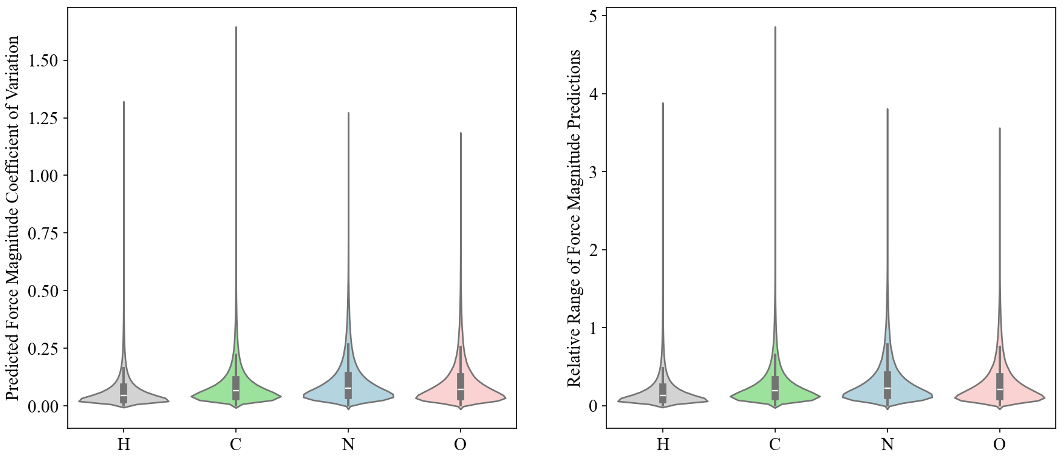
\includegraphics[width=1\linewidth]{Images/2xr_forces/2xr_comp6v1_force-uncertainty_violin.png}
    \caption[Uncertainty in force magnitude predictions: violin distribution]{Violin distribution of force magnitude uncertainty measures (relative standard deviation and relative range), computed for ANI-2xr predictions on the COMP6v1 benchmark dataset.}
    \label{fig:2xr_comp6v1-force_uncertainty-violin}
\end{figure}

Figure \ref{fig:2xr_comp6v1-mean_force_uncertainty_hexbin} presents a direct comparison between per-molecule averaged force uncertainty measures and energy error on the COMP6v1 benchmark dataset. If a clear correlation emerges, these metrics could serve as practical, physics-based uncertainty estimators, enabling more reliable assessments of ANI model reliability without requiring external validation data.

\begin{figure}[!hp]
    \centering
    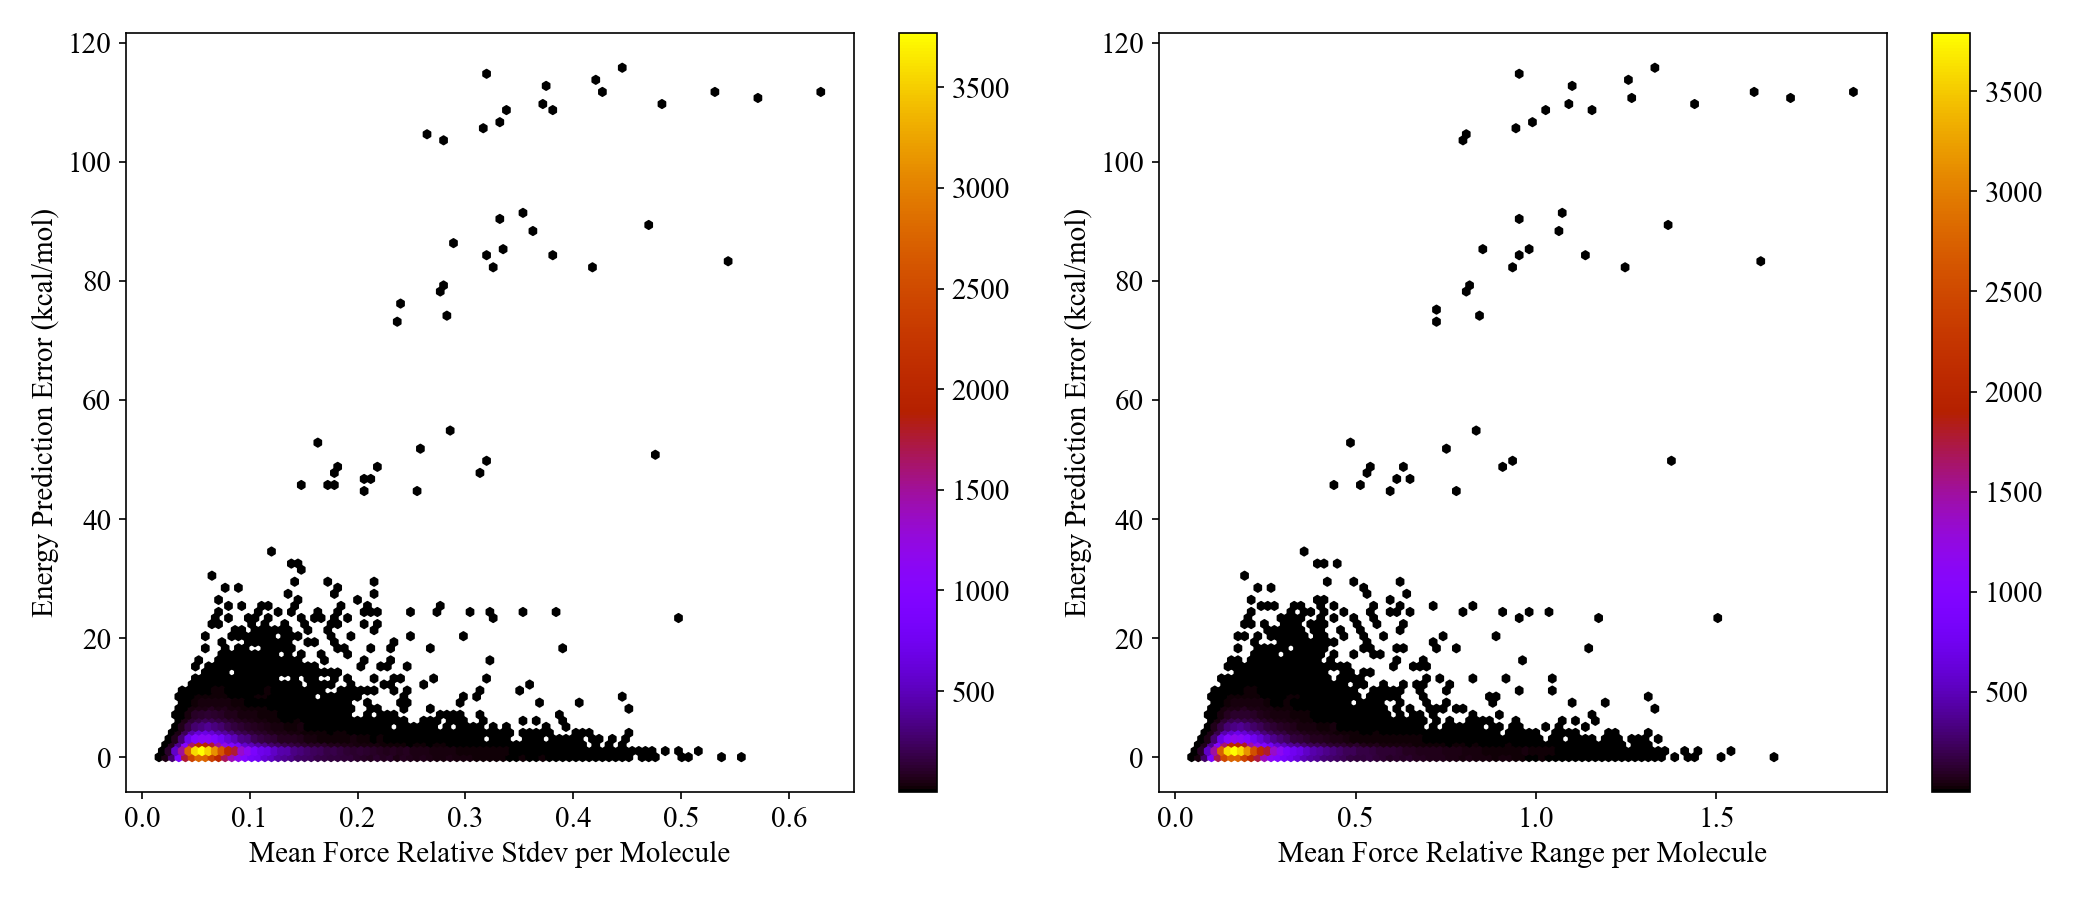
\includegraphics[width=1\linewidth]{Images/2xr_forces/2xr_comp6v1_force-mean-uncertainty-vs-energy.png}
    \caption[Average force uncertainty measures per-molecule versus energy error (COMP6v1)]{Averaged uncertainty measures per-molecule on the ANI-2xr predicted forces versus the energy error for the COMP6v1 benchmark dataset.}
    \label{fig:2xr_comp6v1-mean_force_uncertainty_hexbin}
\end{figure}

To refine our approach further, we explored alternative methods of aggregating atomic force uncertainties at the molecular level. One possibility was to assign greater importance to highly uncertain atomic forces when computing per-molecule uncertainty scores. Figure \ref{fig:2xr_comp6v1-mean_force_uncertainty_hexbin} presents the results of a straightforward averaging approach, where each molecule's force uncertainty is computed as the mean of its atomic uncertainties. While this yielded a reasonable correlation with molecular energy error, we hypothesized that higher-uncertainty atomic forces might contribute disproportionately to poor energy predictions.

To test this, we introduced exponential weighting of atomic force uncertainty measures, increasing the influence of large deviations when computing molecular-level uncertainty. The weighted mean was computed using an exponential function is given in Eqn. \ref{eq:outliers-weighted_sum}.

\begin{equation} 
\mu_{\text{weighted}} = \frac{\sum_i u_i e^{\alpha w_i}}{\sum_i e^{\alpha w_i}} 
\label{eq:outliers-weighted_sum}
\end{equation}

Where $\mu_i$ represents an atomic uncertainty measure (relative standard deviation or relative range), and $w_i$ is a weighting factor, with an adjustable hyperparameter $\alpha$ controlling the strength of weighting. The goal was to emphasize large deviations in atomic force predictions, ensuring that molecules with a few highly uncertain atomic forces would be flagged as high-error cases.


\begin{figure}[!hp]
    \centering
    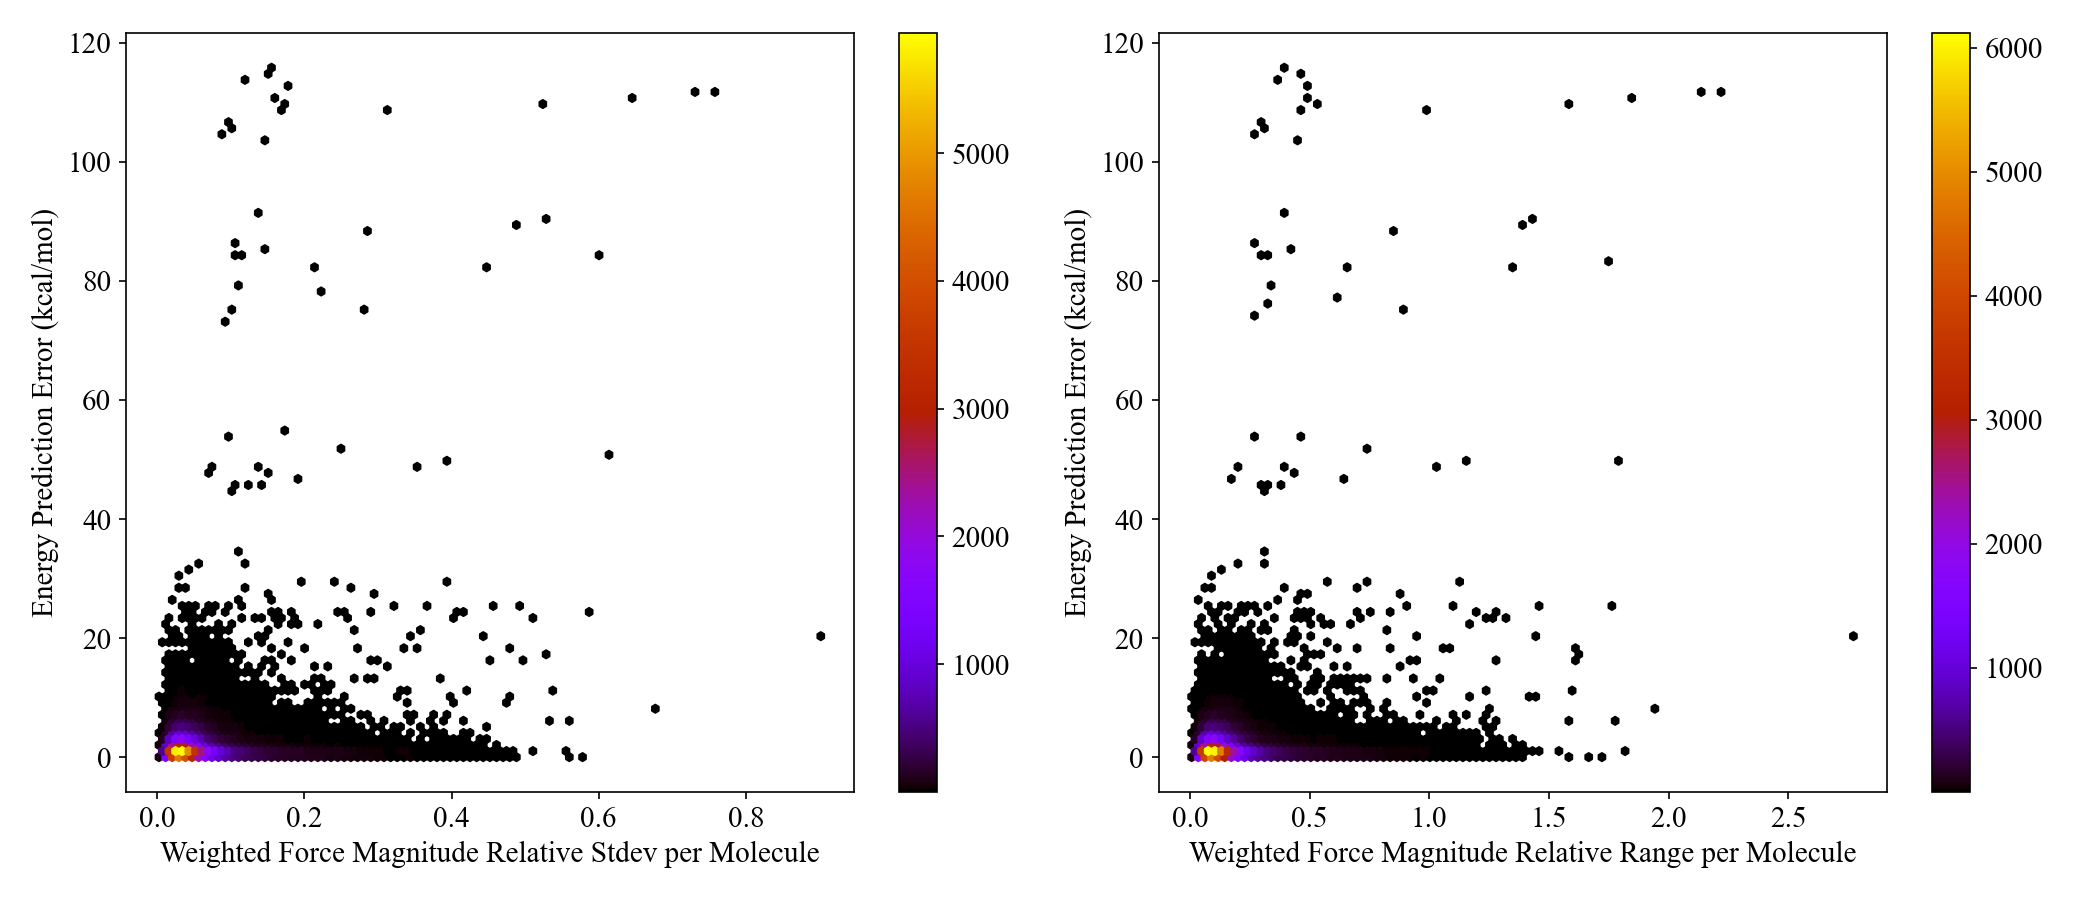
\includegraphics[width=1\linewidth]{Images/2xr_forces/2xr_comp6v1_force-weighted-uncertainty-vs-energy.png}
    \caption[Force uncertainty weighted by outliers versus energy error (COMP6v1)]{Outlier-weighted uncertainty measures for ANI-2xr predicted force magnitudes versus the energy error on the COMP6v1 benchmark dataset.}
    \label{fig:2xr_comp6v1-forces-weighed_uncertainty}
\end{figure}

However, Figure \ref{fig:2xr_comp6v1-forces-weighed_uncertainty} shows that this approach performed worse than simply averaging per-atom uncertainties. The exponential weighting appeared to overemphasize localized outliers, reducing the correlation with molecular energy error rather than improving it. This suggests that large atomic force deviations alone are not always indicative of high molecular uncertainty, and that a different approach was needed.

Given the shortcomings of our weighting approach, we instead focused on capturing the largest single force deviation per molecule. The maximum deviation metric is defined in Equation \ref{eq:max_force_deviation}.

\begin{equation} 
\text{Max deviation} = 
\frac{\left| \left(\max\limits_{m \in {1, \dots, 8}} \vec{F}_{\text{ANI}}^m \right)- \mu_{\text{ANI}} \right|}{\mu_{\text{ANI}}} 
\label{eq:max_force_deviation}
\end{equation}

Where $\vec{F}_{\text{ANI}}^m$ represents the predicted force vector from the $m^{\text{th}}$ model in the ANI ensemble and $\mu_{\text{ANI}}$ represents the mean predicted force magnitude for a given atom across the 8-model ensemble, ensuring that deviations are evaluated relative to the overall prediction spread. The maximum deviation captures the single most extreme disagreement among the ensemble members, highlighting cases where one model significantly diverges from the consensus. By normalizing this deviation by the mean force magnitude, this metric prevents small-force predictions (e.g., near equilibrium) from being overshadowed by inherently larger forces, making it a scale-invariant measure of uncertainty.

Figure \ref{fig:2xr_comp6v1-forces-highest_deviation} presents this maximum deviation measure against molecular energy error. Unlike earlier approaches, this metric highlights cases where at least one atomic force prediction deviates significantly from the ensemble consensus, offering a strong correlation with molecular energy uncertainty.

\begin{figure}[!ht]
    \centering
    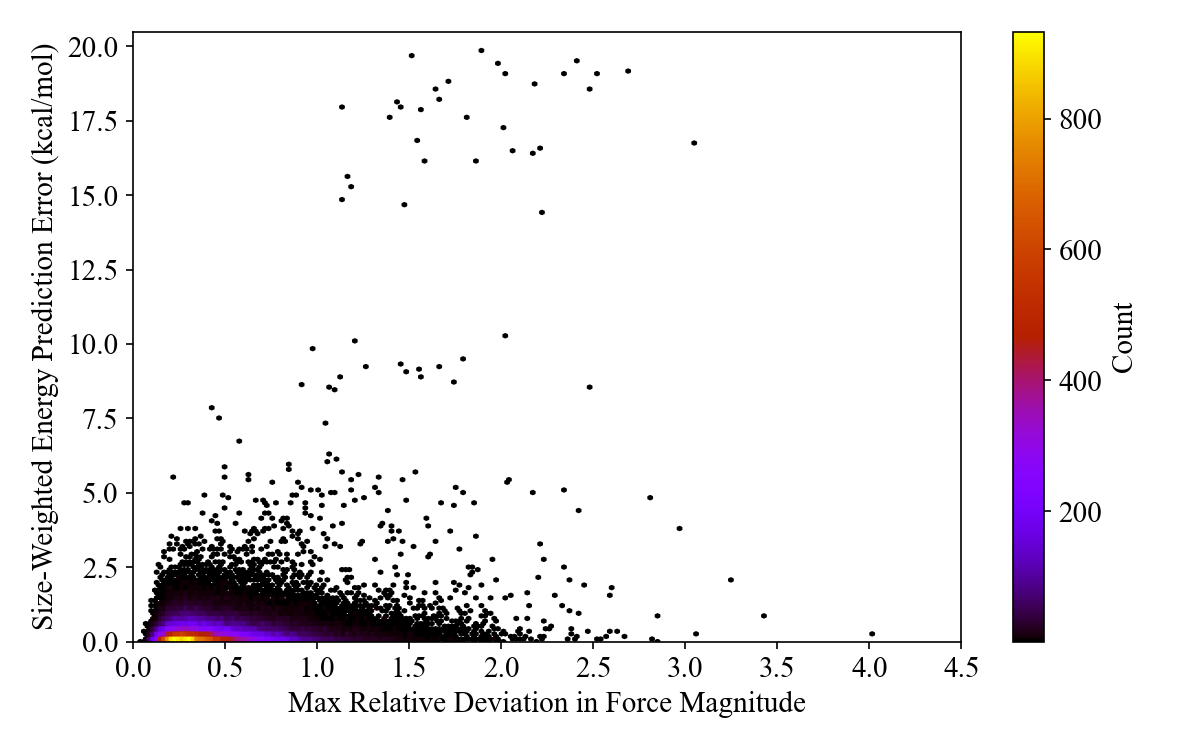
\includegraphics[width=1\linewidth]{Images/2xr_forces/2xr_comp6v1_force-highest-force_deviation-vs-energy.png}
    \caption[Maximum deviation in force magnitude prediction versus energy error (COMP6v1)]{Maximum deviation in force magnitude prediction by ANI-2xr versus energy error on the COMP6v1 benchmark dataset.}
    \label{fig:2xr_comp6v1-forces-highest_deviation}
\end{figure}

The results in Figure \ref{fig:2xr_comp6v1-forces-highest_deviation} demonstrate that the maximum deviation in force magnitude prediction serves as a robust indicator of molecular energy uncertainty. Unlike earlier uncertainty measures that were biased by intrinsic variations in force magnitude, this metric specifically identifies cases where at least one atomic force prediction deviates significantly from the ensemble mean, highlighting regions of the molecule where the model exhibits low confidence. This suggests a crucial improvement to the active learning framework: rather than selecting new training data based on the total energy uncertainty of an entire molecular conformation, we can refine the Query by Committee (QBC) process to target high-uncertainty atomic regions.

The original ANI-1x active learning strategy \cite{ani-1x} leveraged energy-based QBC to identify and sample high-uncertainty molecular structures. However, this approach is limited by its molecule-wide uncertainty aggregation, meaning it treats an entire molecule as either well-represented or underrepresented in the training data. Our findings suggest a more efficient sampling strategy: instead of selecting entire molecules based on total energy uncertainty, we can prioritize the specific conformations where atomic forces exhibit high model disagreement. By refining the active learning process to focus on atomic force uncertainty, we could accomplish three things. (1) Reduce the total amount of required training data while maintaining ANI’s predictive accuracy, similar to the "less is more" approach demonstrated in ANI-1x. (2) Ensure that newly sampled molecules contribute maximally to improving model generalization, by filling in high-uncertainty regions of atomic interactions rather than redundantly adding molecules that contribute little new information. (3) Improve transferability to unseen chemical systems by strategically selecting only the conformers that challenge the model, enhancing its ability to generalize beyond its training set.

The overarching goal is to make ANI equally powerful with less data—a principle demonstrated by the effectiveness of the ANI-1x dataset, which achieved lower molecular energy prediction errors using only a fraction of the original ANI-1 dataset. Applying a similar data-efficient philosophy to force-based uncertainty could significantly accelerate ANI model training and expand its applicability to larger and more diverse chemical spaces. Future iterations of ANI training could incorporate force-based uncertainty quantification into the active learning pipeline, refining data selection to directly address the weakest points of the model. This would not only reduce computational costs but also enhance the overall accuracy and reliability of ANI predictions, ensuring more consistent performance across a wider range of molecular systems.

Having established that atomic force uncertainty serves as a reliable indicator of molecular energy error, the next logical step is to develop a framework for systematically isolating and refining these high-uncertainty regions. Instead of selecting entire molecular structures for retraining, we propose a method to extract and focus on the specific atomic environments that contribute most to uncertainty—a process that could drastically improve the efficiency of the active learning pipeline.

\subsection{Atom Isolator}
\label{subsec:atom_isolator}

To this end, we began developing a tool called Atom Isolator, designed to automatically identify and extract high-uncertainty atoms from molecular structures. The goal of this approach is to refine the active learning process by targeting specific atomic environments rather than entire molecular conformations, thereby improving model accuracy with a smaller, more informative dataset. The first step in this process is identifying high-uncertainty atoms. Using the maximum deviation in force magnitude prediction as a metric, we flag atoms where ensemble disagreement exceeds a given threshold, indicating unreliable model predictions. 

These flagged atoms represent regions where the model is least confident in its force predictions and are therefore the most critical areas to improve. Once these high-uncertainty atoms are identified, the next challenge is truncating the molecular environment in a way that preserves relevant chemical context. Extracting only the flagged atoms would result in a loss of structural information necessary for meaningful predictions. To prevent this, Atom Isolator defines a tunable cutoff radius around each high-uncertainty atom, set to approximately 1.5 times the AEV cutoff. 
An example of this is given in Figure \ref{fig:atom_isolator}.

\begin{flushleft}
\begin{multiFigure}
\begin{centering}
    \addFigure{0.4}{Images/atom_isolator/c2h3n7o2-cropped.png}
    \addFigure{0.4}{Images/atom_isolator/c2h3n7o2_highlighted-cropped.png} 
    \addFigure{0.4}{Images/atom_isolator/c2h3n7o2_11isolator-cropped.png}
    \addFigure{0.4}{Images/atom_isolator/c2h3n7o2_2isolator-cropped.png} \\
\captionof{figure}[Example output from the atom isolator]{(A) C\textsubscript{2}H\textsubscript{3}N\textsubscript{7}O\textsubscript{2} molecule from ANI dataset, (B) atoms with a high force uncertainty value, and the atom isolator output from (C) atom 2 and (D) atom 11. Note that some of the molecule is truncated at the AEV cutoff in either case; refer to Fig. \ref{fig:aev_radius} for an example of this cutoff radius.
}
\label{fig:atom_isolator}
\end{centering}
\end{multiFigure}
\end{flushleft}

\authorRemark{This ensures that enough of the local atomic environment is retained to maintain chemically meaningful interactions, while avoiding unnecessary contributions from well-learned regions of the molecule. Finally, these extracted atomic environments are treated as independent molecular fragments, which can be reintroduced into the training process. By isolating and refining only the most uncertain atomic regions, this approach prioritizes data sampling where the model struggles most, rather than redundantly retraining on entire molecular structures that contain many well-predicted regions. This focused data augmentation strategy has the potential to significantly reduce dataset size while maintaining or even improving predictive accuracy.}


The process of isolating high-uncertainty atomic environments presents an opportunity to search for reduced molecular representations that retain the key chemical patterns associated with high-uncertainty predictions. Instead of retraining the ANI model on large, computationally expensive structures, we can use these fragmented environments to identify simpler molecular motifs that capture the essential bonding interactions contributing to uncertainty. This approach aligns with broader trends in molecular AI research, where efforts to develop compressed molecular representations have led to advances in AI-driven drug discovery \cite{mol_reps_in_AI_drug_discovery_david} and systematic chemical pattern matching through SMILES and SMARTS representations \cite{SMILES_pair_encoding_li, mol_patterns_SMARTS_schmidt, automated_fragment_gen_smiles_bilsland}.

One potential application of this method is to build a database of high-uncertainty motifs, which could guide targeted data augmentation by focusing additional QM calculations on molecular substructures that ANI struggles to learn. By leveraging direct chemical perception techniques, such as those proposed by Mobley et al. \cite{direct_chem_perception_mobley}, we could further refine how we define chemically relevant fragments, moving away from conventional atom-typing approaches in favor of AI-driven adaptive fragmentation. An additional challenge in this workflow is ensuring that the truncated molecular fragments remain chemically valid after removal from their original structure. When an atom is extracted from a larger molecule, its local bonding environment is disrupted, potentially leading to unrealistic chemical representations. To address this, we explored capping the truncated fragments with hydrogen atoms, a common strategy in force field parametrization and molecular fragmentation \cite{protein_ff_fragmentation_nn_wang}.

Hydrogen capping provides a straightforward way to satisfy valency constraints and maintain a chemically reasonable representation of the isolated substructure. However, this modifies the local atomic environment, altering the AEV input representation that the ANI model originally learned from. This poses a fundamental challenge: while capping ensures that the fragment is a well-defined molecule, it may no longer resemble the high-uncertainty environment that necessitated its selection in the first place. To mitigate this issue, we investigated identifying neighboring atoms beyond the AEV cutoff radius and incorporating their influence into the truncated system. The idea was that, rather than directly capping with hydrogen atoms, we could preserve electronic effects from adjacent atoms by selecting neighbors beyond the standard AEV interaction range. This would maintain the fragment’s chemical context without introducing artificial changes to its bonding patterns.

Developing an automated approach to extracting and refining high-uncertainty fragments could significantly improve active learning strategies for ANI models. By focusing on substructures that contribute most to model uncertainty, we can enhance predictive accuracy while minimizing computational cost. Future work will involve integrating pattern-recognition algorithms for detecting recurring uncertainty motifs, leveraging SMILES-based matching methods \cite{SMILES_pair_encoding_li} to identify chemically similar environments that may require additional training data. Ultimately, Atom Isolator represents a step toward precision-driven model refinement, where retraining efforts are concentrated on the most challenging chemical motifs rather than entire molecules. By developing a framework that systematically isolates, refines, and reintegrates uncertain atomic environments, we aim to reduce dataset redundancy while improving the robustness and generalizability of ANI predictions.

\subsection{Drawback: Configurational Sampling}
\label{subsec:drawback_config_sampling}

While the Atom Isolator approach offers a focused strategy for identifying and retraining high-uncertainty atomic environments, it presents a fundamental limitation: the lack of diverse configurational sampling. By extracting and truncating molecular substructures, we improve the representation of high-error atomic environments but do little to expand the broader diversity of molecular configurations that ANI encounters during inference. This raises a crucial question: Is targeting only localized uncertainty enough to enhance the generalizability of ANI models, or do we also need a systematic way to introduce new molecular configurations?

A fundamental distinction in molecular datasets is the difference between conformational and configurational diversity. Conformational sampling refers to generating different 3D structures (rotamers) of a given molecule, such as exploring torsional rotations around flexible bonds, bending of molecular frameworks, or sampling vibrational distortions near equilibrium geometries. While this form of sampling is important, it is inherently limited to a fixed set of molecular graphs, meaning that it does not expand the diversity of molecular connectivity patterns available to the model. Historically, ANI datasets—including ANI-1 \cite{ani-1} and ANI-2x \cite{ani-2x}—have relied heavily on conformational sampling to enrich training data. The molecules in these datasets were sourced from large enumerated molecular databases, such as GDB-13 \cite{gdb-13} and GDB-17 \cite{gdb-17}, which contain systematic lists of all possible stable organic molecules up to a given number of heavy atoms. These datasets provide exhaustive coverage of stable molecules with up to 13 or 17 heavy atoms, respectively, ensuring that small organic structures are well-represented.

However, a major issue with this approach is dataset redundancy. The GDB databases were designed for small molecule discovery and drug-like compounds, meaning that a vast majority of the structures they contain exhibit similar functional groups and molecular motifs. The result is an oversampling of certain chemical environments, leading to a model that performs well on common molecular patterns but struggles when exposed to molecules that differ significantly from those in training. The consequence of this presents a hole in configurational diversity—the model lacks exposure to entirely new molecular architectures. If we only expand the training set through conformational sampling, we remain constrained to a narrow region of chemical space, improving accuracy within that limited domain but failing to generalize beyond it. This means that ANI models will inevitably encounter molecules during inference that fall well outside their learned chemical space, leading to poor extrapolation and unreliable predictions for novel molecules.

To truly enhance ANI’s reliability, we need to go beyond conformational sampling and introduce configurational sampling—the process of systematically expanding the molecular connectivity space that the model has access to. While conformational sampling ensures that a given molecule’s low-energy geometries are well-represented, configurational sampling ensures that a model encounters diverse bonding topologies, functional group variations, and novel molecular frameworks.

A promising source of configurational diversity is ChEMBL \cite{ChEMBL_gaulton}, a large database of bioactive molecules with experimentally validated drug-like properties. Unlike GDB-derived datasets, which primarily contain small, stable organic molecules, ChEMBL includes a broader range of chemically relevant structures, including pharmacophores and complex heterocycles commonly found in medicinal chemistry, reactive intermediates and metabolites, which provide insights into chemical reactivity, and transition-state-like geometries, which are critical for understanding reaction dynamics. By incorporating ChEMBL-derived molecules into the training process, we can expand ANI’s knowledge of chemical space, enabling it to generalize more effectively to novel compounds.

Another approach to increasing configurational diversity is the systematic generation of new molecular fragments based on high-uncertainty atomic environments. As explored in the Atom Isolator section, truncated high-uncertainty regions provide insight into molecular motifs that challenge ANI’s predictions. If we can map these motifs to larger molecular frameworks, we may be able to generate new molecules that share key bonding characteristics but provide fresh chemical contexts for model training.

This discussion leads to a critical consideration: If ANI models struggle most in specific atomic environments, should active learning strategies focus on fine-tuning the model using extracted high-error substructures, or should they instead prioritize generating novel configurations that explore previously unseen regions of chemical space? The Atom Isolator approach enhances model refinement, but it does not necessarily expand the configurational diversity of the training set.

A more balanced solution may involve a hybrid approach—using high-uncertainty atomic fragments as a guide for selecting new molecular configurations from external databases, allowing the model to learn from both localized uncertainty and broader molecular diversity. This concept is explored in greater depth in Section \ref{sec:exploring_new_mol_configs}, where we examine how configurational sampling methods can be leveraged to improve ANI’s coverage of the potential energy surface.

\section{Outlook}

The exploration of uncertainty in ANI predictions has revealed both the strengths and limitations of current ensemble-based approaches. While total molecular energy uncertainty, measured via query by committee (QBC), has been a useful heuristic for active learning, our investigation has shown that atomic force uncertainty provides a more physically meaningful alternative. By shifting the focus from total energy deviations to localized force-based uncertainty measures, we have outlined a potential pathway toward more targeted and data-efficient model training strategies.

The development of the Atom Isolator provides a first step in refining active learning strategies, allowing us to focus training on high-uncertainty regions of molecular space rather than entire conformational ensembles. However, as discussed in Section \ref{subsec:drawback_config_sampling}, this approach alone does not fully address the need for configurational diversity in ANI training. Moving forward, an integrated approach—combining uncertainty-driven atomic substructure selection with configurational expansion strategies—may offer the most efficient path toward improving model generalization.

Beyond training set refinement, the uncertainty quantification methods explored in this work could also facilitate the expansion of ANI models to include additional elements, most notably phosphorus, which would enable the accurate simulation of RNA, DNA, and other biomolecular systems. The ability to systematically detect regions of high uncertainty provides a powerful tool for identifying failure modes in ANI predictions before they impact large-scale simulations. By applying these uncertainty-driven strategies, we could prioritize high-uncertainty phosphorus-containing structures for new data generation, ensuring that ANI models gain reliable predictive power in nucleotides, phosphate-containing cofactors, and other biologically relevant molecules.

With phosphorus incorporated into the ANI framework, ANI-based potentials would become directly applicable to the study of genetic materials, unlocking high-fidelity molecular dynamics (MD) simulations of RNA folding, DNA stability, and nucleotide interactions. The ability to capture long-timescale structural rearrangements in complex biomolecules—at a fraction of the computational cost of traditional quantum mechanical approaches—would significantly enhance large-scale biochemical modeling. Moreover, these improvements could extend beyond nucleic acids, refining ANI’s applicability to organophosphates, phosphate esters, and other reactive phosphorus-containing species that play critical roles in enzymatic catalysis, prebiotic chemistry, and metabolic pathways.

By leveraging physically interpretable uncertainty metrics, we can refine data selection strategies to efficiently expand ANI's chemical scope, enhance model reliability in complex biological environments, and accelerate the development of machine-learned potentials capable of scaling to new frontiers in biomolecular and reactive chemical simulations. While achieving this will require a balance between data efficiency and chemical diversity, the methods presented in this chapter suggest a clear pathway toward constructing the next generation of ANI models with significantly broader applicability.%
\chapter{LAMMPS-ANI Early Earth Chemistry} 

\section{CUDA-accelerated atomic environment vectors}

\section{GPU parallelization}

\section{ANI-1xnr}

\section{The Miller Experiment}%
\chapter{Hero Run Data Analysis} 
\label{chapter5}

The fully scaled version of the Early Earth simulation, referred to as the HiPerGator Hero Run, represents the most extensive molecular dynamics (MD) simulation ever conducted with a machine-learned interatomic potential. This ambitious project was a collaboration between the HiPerGator research computing team, NVIDIA, and the Roitberg group, leveraging cutting-edge GPU technology and state-of-the-art neural network potentials to model prebiotic chemistry on an unprecedented scale.

The Hero Run was conducted over six days, utilizing thousands of GPUs across the entire HiPerGator supercomputer to simulate 4.5 nanoseconds of reactive molecular dynamics. The temperature profile of the simulation was carefully designed to mimic potential prebiotic reaction conditions, incorporating both high-temperature chemistry and cooling cycles to explore the formation and stability of complex molecular species. The timeline of the simulation included: 0.05 ns heating from 0 K to 300 K, 0.2 ns heating from 300 K to 2500 K, 4.0 ns at 2500 K allowing extensive bond rearrangement, finally 0.25 ns cooling back to 300 K enabling the analysis of stable reaction products.
This temperature cycle was selected based on experimental and computational studies of high-energy impact chemistry, where transient high temperatures enable chemical bond rearrangement, followed by rapid cooling to capture stable reaction products.

The simulation encompassed a massive 22.8 million atoms, making it one of the largest reactive MD simulations ever conducted. ANI-1xnr, a machine-learned interatomic potential, provided near-quantum accuracy while maintaining the efficiency required to run such an extensive system. However, running a simulation at this scale posed significant computational challenges.
The next sections detail the strategies developed to process, analyze, and extract meaningful insights from this unprecedented dataset, including graph-based molecular identification, GPU-accelerated trajectory filtering, and large-scale clustering techniques.

\section{Molfind}
\label{sec:molfind}

MolFind is a protocol written in Python with RAPIDS 
%[cite] 
GPU-accelerated libraries which operates by translating each simulation snapshot into a graph data structure on the GPU, where atoms are represented as graph vertices and pairwise interactions (e.g., bonds or neighbor connections) become edges. To construct this graph, the tool leverages GPU-based neighbor-list building, using either cell-list or cutoff methods, and then uses the cuGraph library to create and store the adjacency information in GPU memory. Once the atom-level graph is established, MolFind performs connected-component searches to identify sets of atoms that form discrete molecular fragments, thus mapping the complex MD snapshot into discrete graph partitions. After extracting these connected subgraphs, it computes a flattened chemical formula for each fragment by collecting and sorting atomic species, which helps identify the basic stoichiometry. To capture structural details beyond mere composition, MolFind also assembles a “signature” string that encodes the internal connectivity—each bond is represented in a standardized format (e.g., sorted alphabetically as “C-H”) and aggregated to form a reproducible fingerprint. This combination of stoichiometric and connectivity descriptors ensures that fragments with identical compositions but different bond arrangements (e.g., isomers) can be distinguished. Finally, if desired, MolFind compares each fragment’s subgraph to a prebuilt reference database of molecular graphs. These comparisons involve GPU-accelerated manipulations and, where necessary, a final CPU-based isomorphism check with the NetworkX library 
%[cite] 
to verify exact structural matches. By keeping the core graph-building and connected-component search on the GPU, MolFind can scale to millions of atoms, enabling users to sweep through extended trajectories, track how molecular species evolve over time, and detect rare or unexpected products in large reactive systems.

\subsection{GraphMatcher}
\label{subsec:molfind_graphmatcher}

The GraphMatcher step in MolFind is responsible for determining whether a newly discovered fragment in a simulation matches any of the reference molecules in a provided database. After extracting the topology of each fragment as a graph (where nodes are atoms and edges represent bonds), MolFind adorns edges and nodes with additional labels—nodes store the atomic element, and edges store the bonded element pair (e.g., $\text{C–N}$, $\text{H–O}$). The tool then constructs an equivalent “reference graph” for each known molecule in the database, storing the same node and edge attributes. The matching procedure uses NetworkX’s GraphMatcher, specifically a categorical node match and categorical edge match strategy, to ensure that corresponding atoms and bonds must have the same chemical identity for the two subgraphs to be considered isomorphic. If the subgraph is determined to be isomorphic to a reference, MolFind assigns the corresponding label (e.g., “alanine” or “glycine”) to the fragment. 

In early development, some structures were mistakenly identified as alanine (Figure \ref{fig:mismatched_alanine}), underscoring the importance of carefully specifying node and edge attributes and verifying the molecular configuration.

\begin{flushleft}
\begin{multiFigure}
    \addFigure{0.5}{Images/early_earth/remakenot_alanine.png}
    \addFigure{0.5}{Images/early_earth/remakenot_alanine_silhouette.png}
\captionof{figure}[Mismatched structure of alanine]{
(A) Structure identified as alanine; 
(B) how the GraphMatcher was interpreting this structure, which makes it appear to be an alanine molecule.}
\label{fig:mismatched_alanine}
\end{multiFigure}
\end{flushleft}

In particular, if nodes were not distinctly labeled by their atomic species, or edges were not checked for precise element pairs, the GraphMatcher could falsely declare an isomorphism, conflating dissimilar fragments. By refining the graph-building procedure—ensuring that each node had the correct element label and each edge the correct pair of elements—MolFind began to more accurately match molecules in large-scale simulations. This adjustment led to corrected counts for species originally overestimated due to misidentification (Figure \ref{fig:graph_matching}). In practice, once node and edge attributes are rigorously assigned, the GraphMatcher becomes a powerful method for confirming the presence of specific molecules within highly complex molecular dynamics trajectories.

\begin{figure}[!ht]
    \centering
    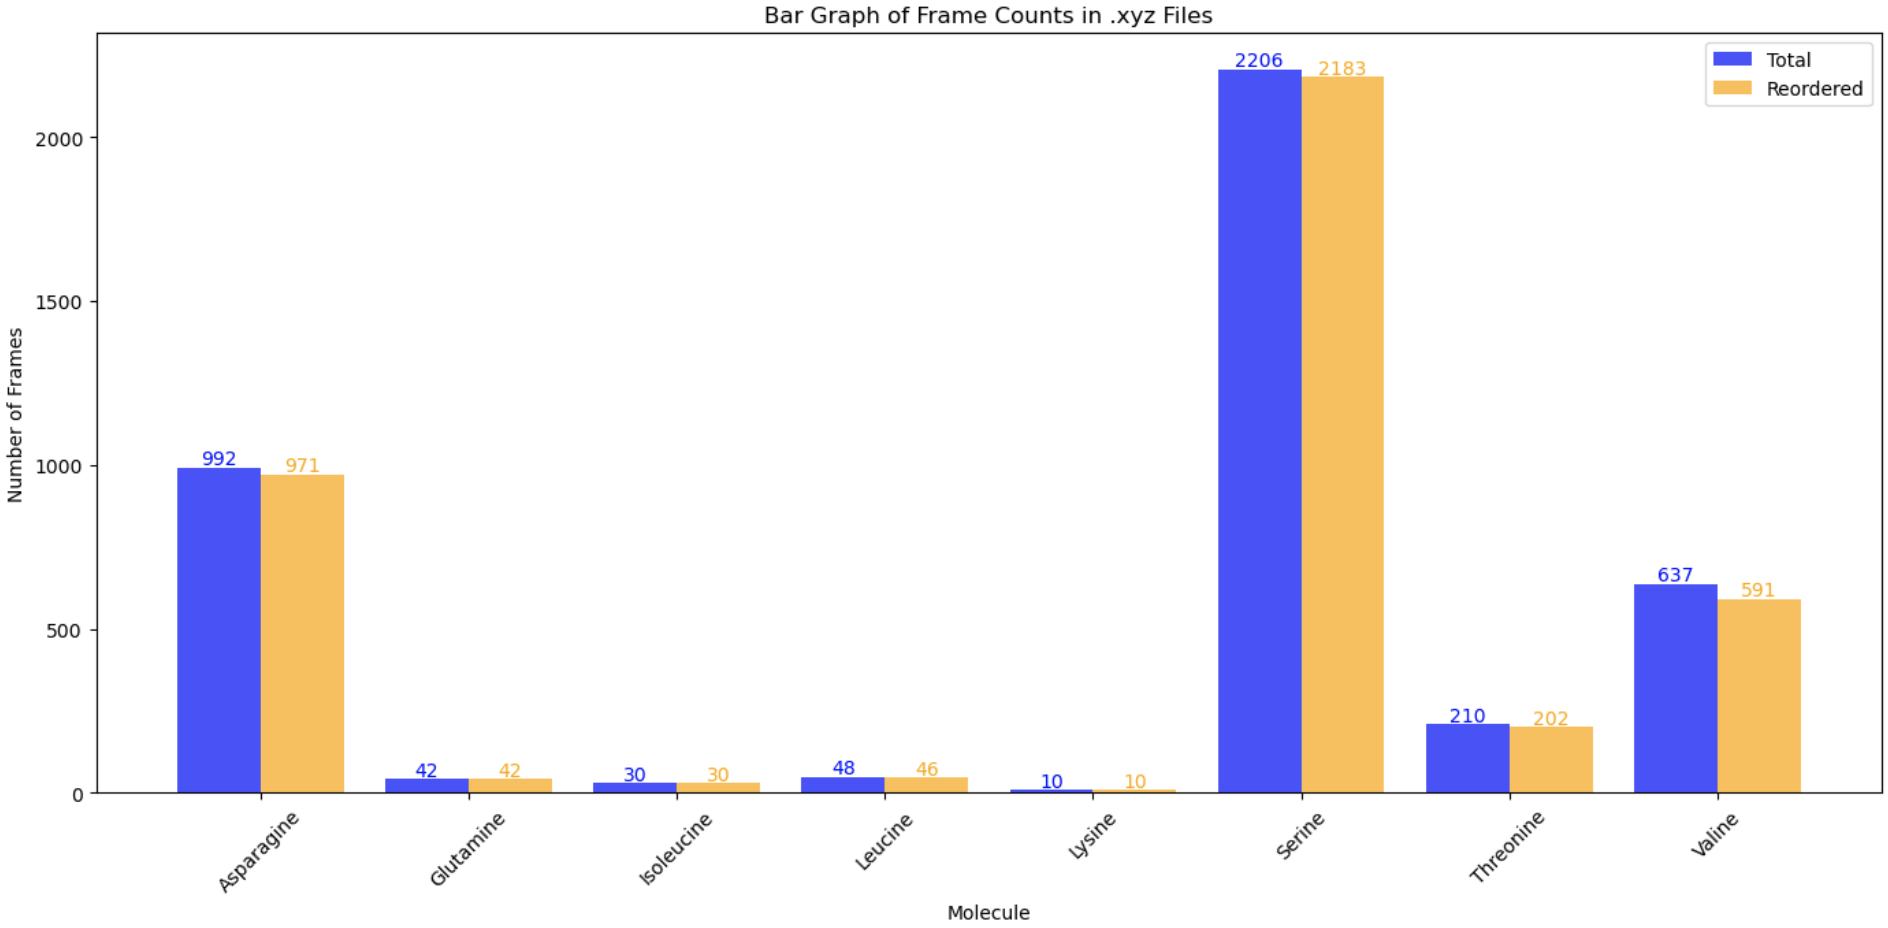
\includegraphics[width=1\linewidth]{Images/early_earth/remake_graph_matching.png}
    \caption[Molecules identified incorrectly in the initial search]{Molecule counts (excluding glycine and alanine) before and after correcting the graph-matching algorithm to account for the proper configuration.}
    \label{fig:graph_matching}
\end{figure}{}

With the corrected graph-matching procedure in place, the identification of alanine molecules in the simulation is now more reliable, allowing for a detailed analysis of their structural properties. 

\begin{figure}[!ht]
    \centering
    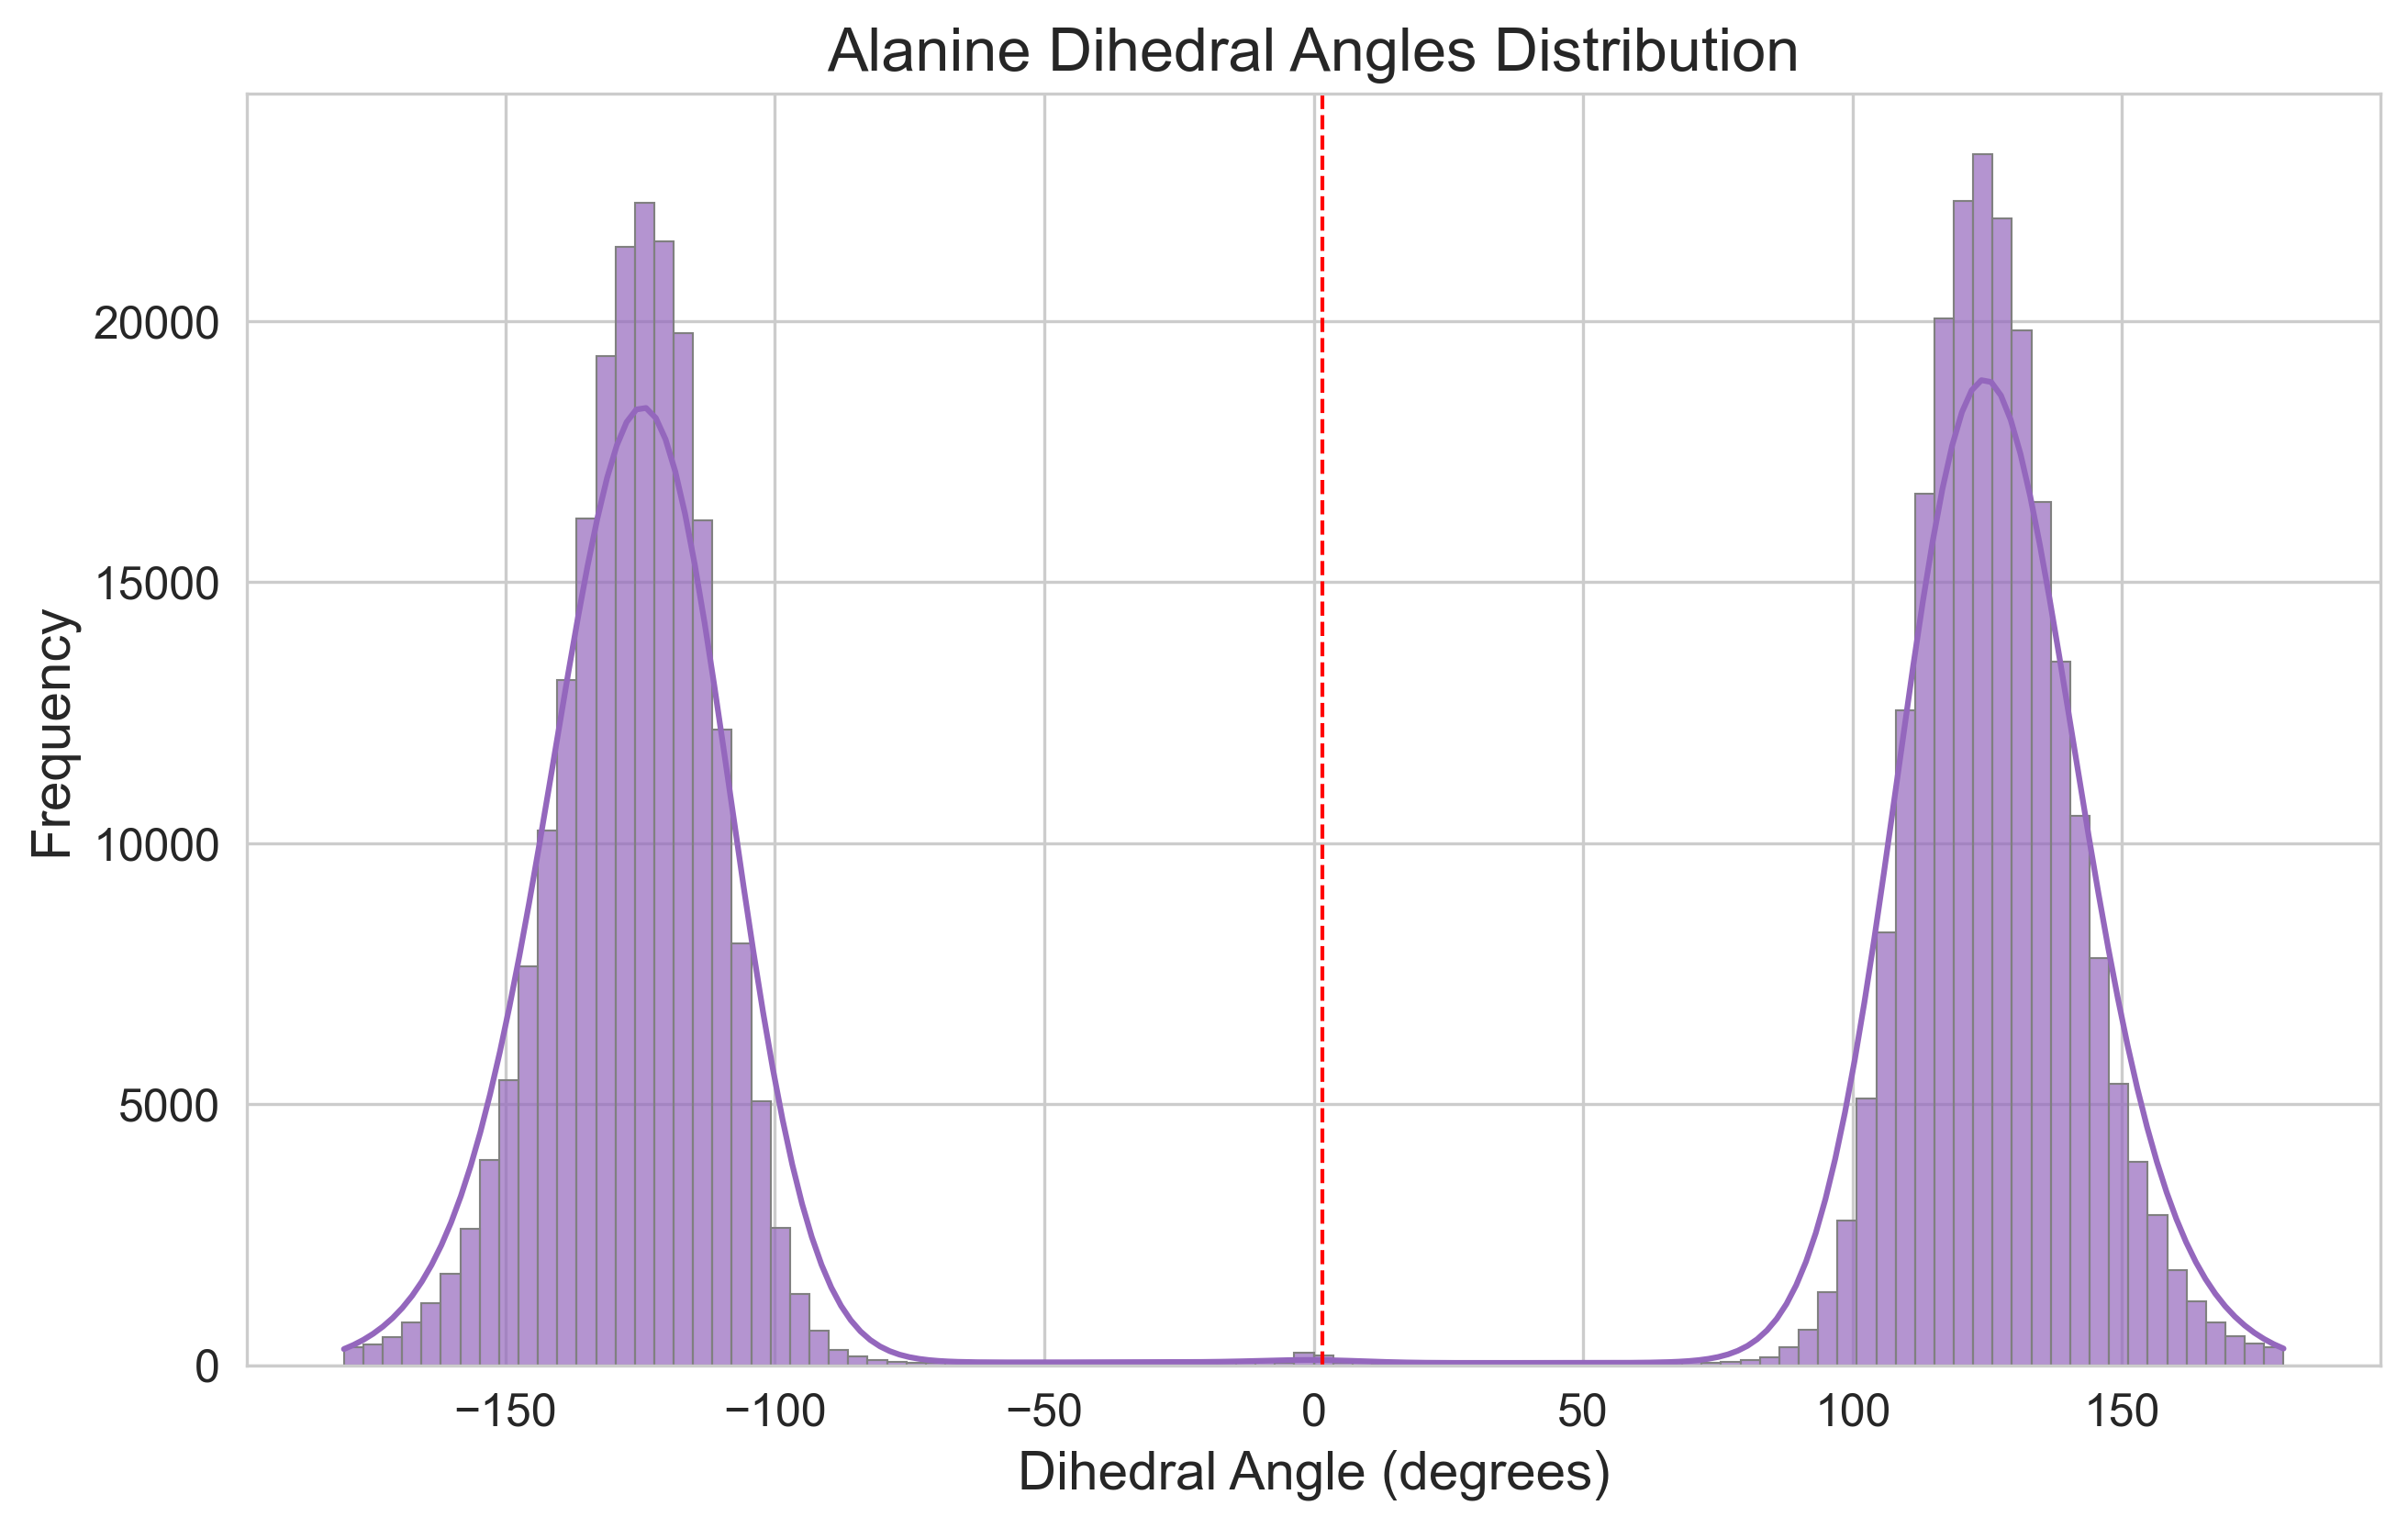
\includegraphics[width=1\linewidth]{Images/alanine_dihedral/dihedral_angles_distribution.png}
    \caption[Distribution of synthesized alanine dihedral angles]{Distribution of dihedral angles in alanine molecules synthesized in the early earth simulation run. Structures obtained from the initial graph search, post-processed with refined graph matching. All molecules fall within the expected range of dihedral angles, centered at $\pm$125$^\circ$.}
    \label{fig:ala_dihedral}
\end{figure}

From the approximately 500,000 alanine molecules synthesized in the Early Earth hero run, dihedral angles were measured to assess conformational distributions. As shown in Figure \ref{fig:ala_dihedral}, the dihedral angles cluster around $\pm$125$^\circ$, consistent with expected alanine geometries. This analysis confirms that the molecular structures identified through the refined graph search not only match the expected connectivity patterns but also exhibit realistic conformational behavior, further validating the accuracy of the updated graph-matching approach.

\subsection{Parallelization}
\label{subsec:molfind_parallelization}

To efficiently process the vast amounts of molecular data generated in the Early Earth simulation, MolFind leverages GPU-accelerated computing through the RAPIDS ecosystem, specifically cuGraph and cuDF, to minimize CPU bottlenecks and perform large-scale graph analysis directly on the GPU. The core of the molecular identification workflow—constructing atomic graphs, finding molecular fragments, and analyzing connectivity—is executed using cuGraph, which provides highly optimized, massively parallel algorithms for graph operations. Instead of iterating through millions of atomic interactions on the CPU, cuGraph’s connected component search rapidly groups atoms into discrete molecular fragments, enabling near-instantaneous classification of structures.

Once fragments are identified, cuDF is used  to store and manipulate molecular descriptors, allowing for rapid filtering, sorting, and aggregation of molecular data while remaining in GPU memory. Unlike traditional CPU-based approaches, which require costly data transfers between RAM and GPU memory, cuDF enables columnar data operations directly within GPU memory, accelerating tasks such as counting molecular occurrences, applying transformations to chemical formulas, and merging results with reference databases. The entire pipeline—from reading molecular dynamics trajectories to identifying molecules and performing statistical analysis—remains within the GPU as much as possible, significantly reducing computation time compared to CPU-bound methods. By using RAPIDS' GPU-native tools, MolFind achieves a scalable approach to analyzing tens of millions of atoms across thousands of trajectory frames, making high-throughput molecular discovery feasible for large-scale simulations.

\section{Restarts -- Quench analysis}
\label{sec:restarts_quench_analysis}

In the Early Earth simulation, 415 selected frames from the 22.8-million-atom system were quenched from 2500 K to 300 K, allowing us to observe how molecular structures stabilize at lower temperatures. The histograms in Figure \ref{fig:ee_quench_hist} compare the distribution of named molecules before and after quenching, highlighting a significant increase in molecular complexity. 

\begin{figure}[!h]
    \centering
    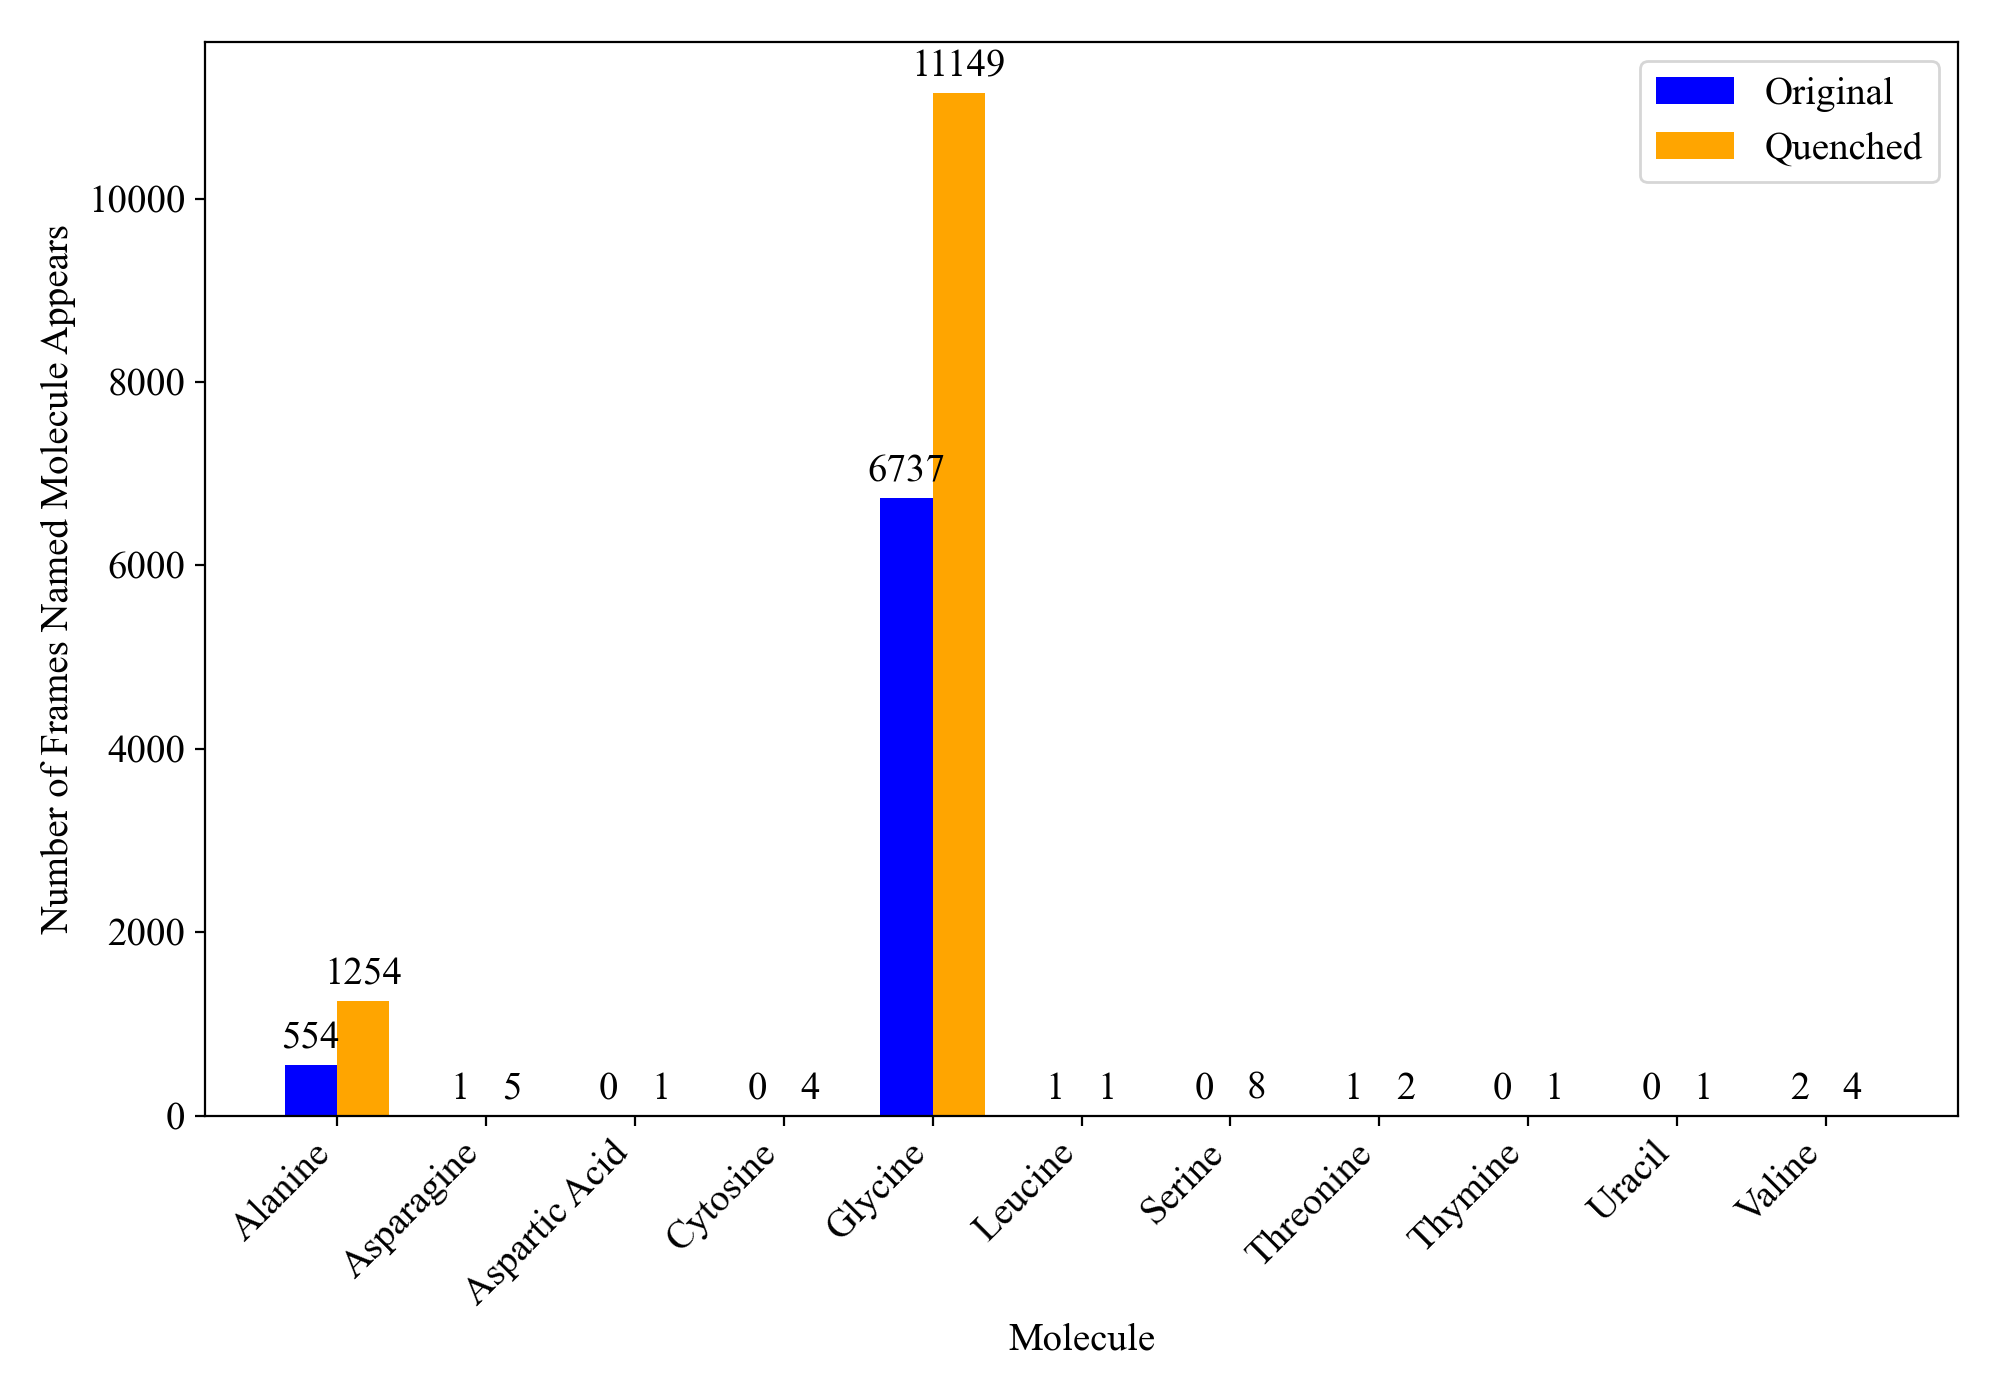
\includegraphics[width=1\linewidth]{Images/early_earth/hist-before-after-quench.png}
    \caption[Histogram: molecules found before and after quenching system]{Histogram of named molecules found before and after quenching 415 selected frames from the 22.8M atom system from 2500 K to 300 K.}
    \label{fig:ee_quench_hist}
\end{figure}

Many smaller fragments coalesced into larger molecules, with a notable rise in carbon-based structures, suggesting that polymerization and oligomerization events occur as the system cools.
This transition is further illustrated in Figure \ref{fig:ee_quench_lineplot}, which tracks the total per-frame count of named molecules before and after the quench. While the total number of individual fragments decreased after cooling, the presence of larger, more chemically diverse molecules increased, indicating that higher-order molecular assembly is favored at lower temperatures.

\begin{figure}[!h]
    \centering
    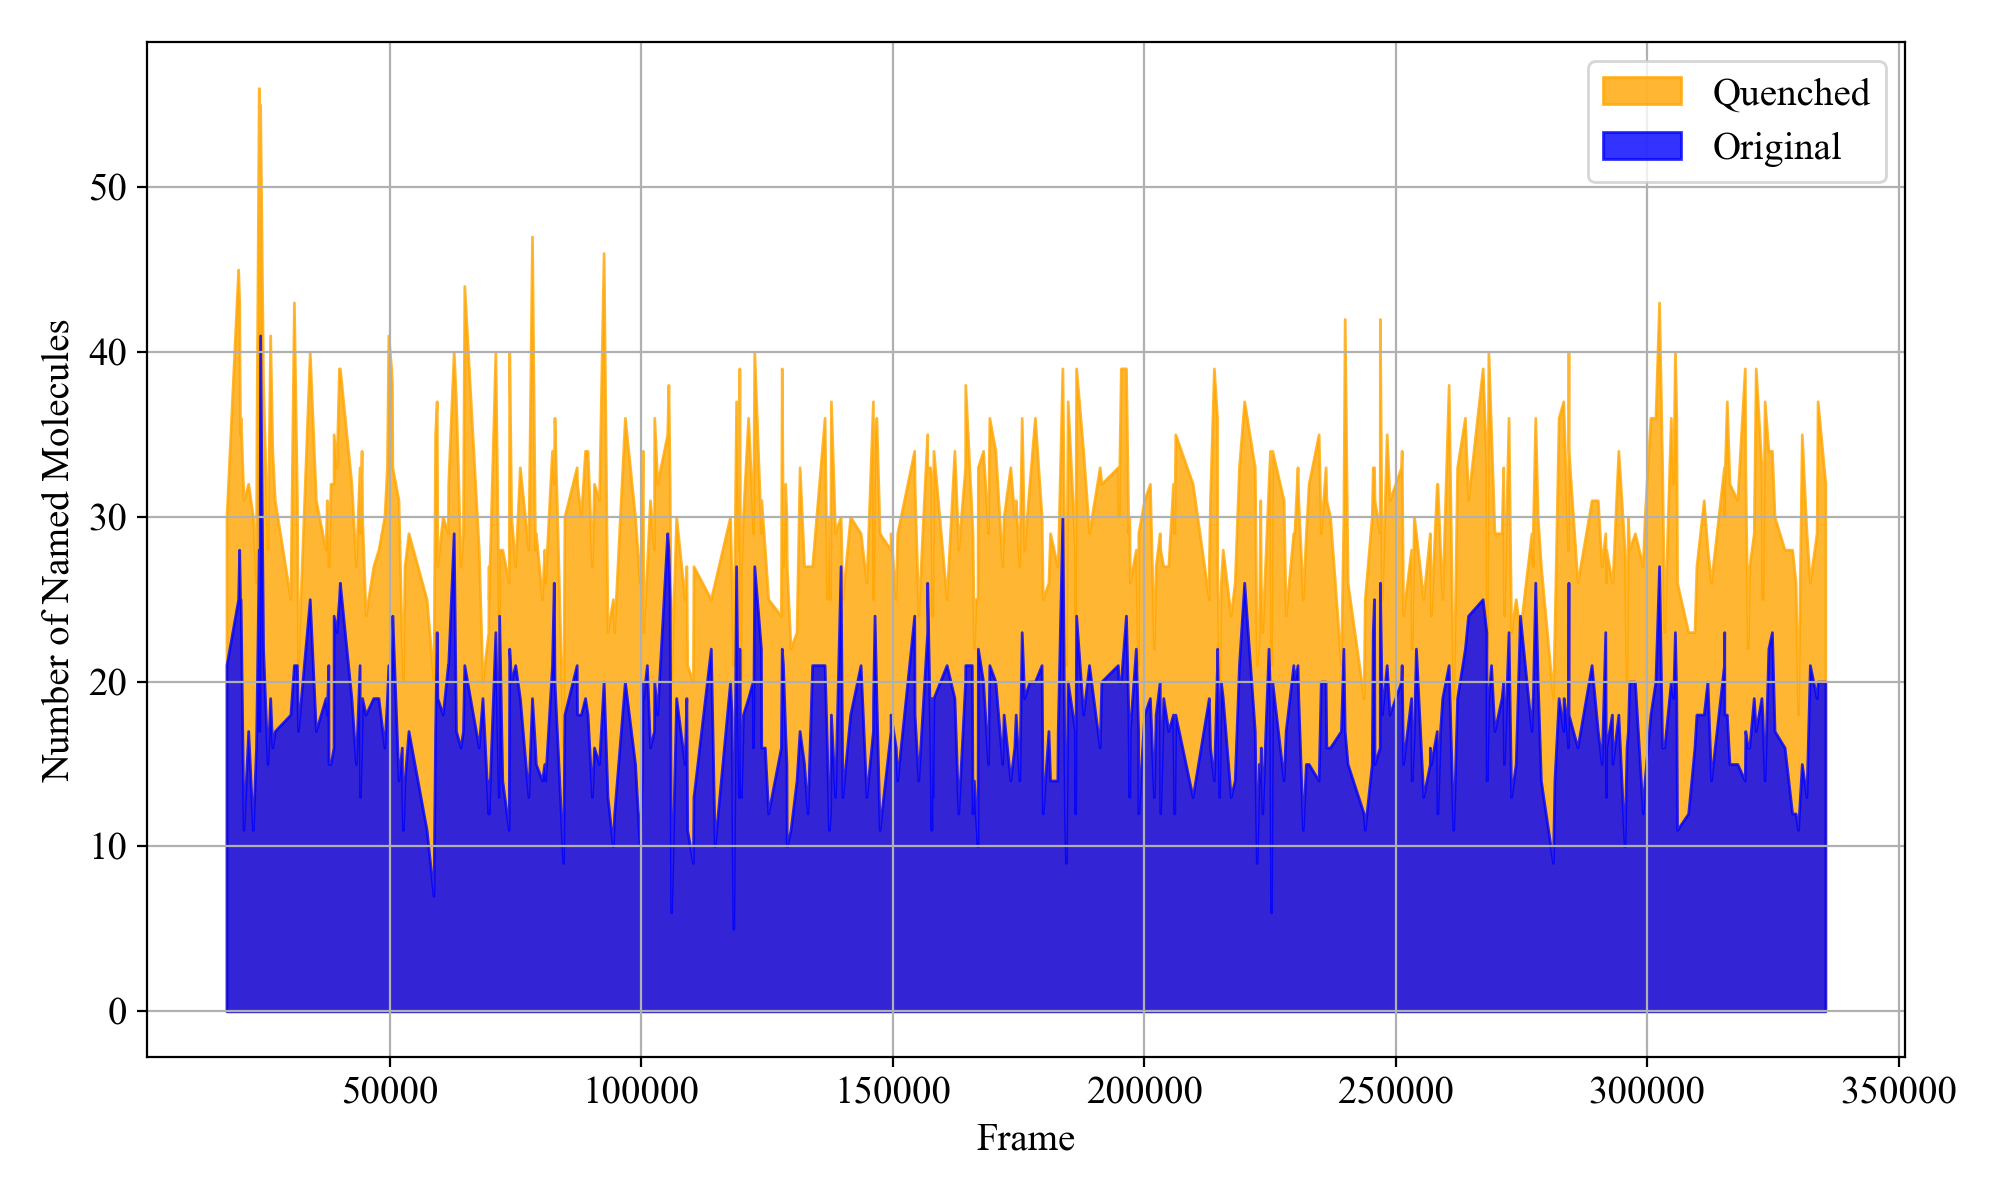
\includegraphics[width=1\linewidth]{Images/early_earth/mol_counts-before-after-quench.png}
    \caption[Line plot: total named molecules found before and after quenching system]{Total per-frame count of named molecules found before and after quenching 415 selected frames from the 22.8M atom system from 2500 K to 300 K.}
    \label{fig:ee_quench_lineplot}
\end{figure}

Prior to quenching, molecular fragments were smaller and more transient, with an average molecule size of 18 atoms per fragment, reflecting the high degree of fragmentation and reactive dynamics at elevated temperatures. However, following the temperature drop, the system exhibited a shift toward larger and more stable molecular species, with the average fragment size increasing to about 30 atoms per molecule in each frame as demonstrated in Figure \ref{fig:ee_quench_violinplot}.

\begin{figure}[!ht]
    \centering
    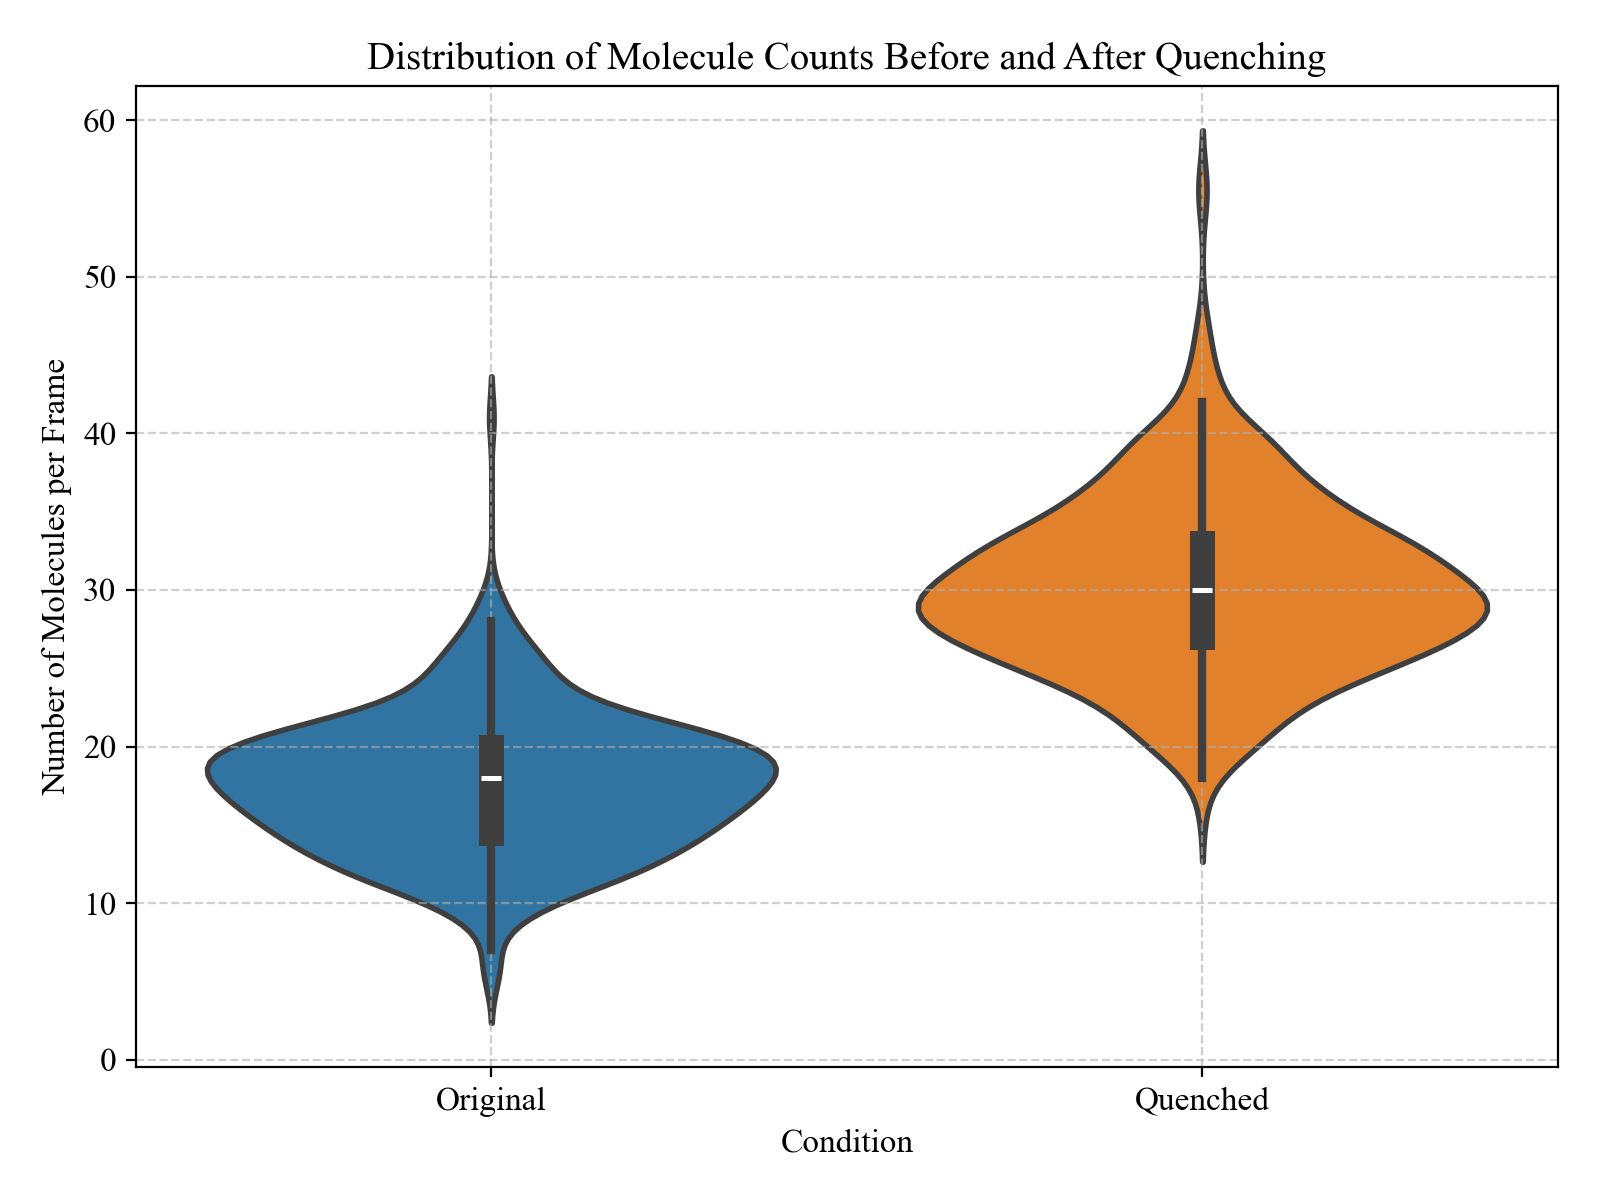
\includegraphics[width=1\linewidth]{Images/early_earth/violinplot-mol_counts-before-after-quench.png}
    \caption[Violin plot: total named molecules found before and after quenching system]{Distribution of per-frame counts of named molecules found before and after quenching 415 selected frames from the 22.8M atom system from 2500 K to 300 K.}
    \label{fig:ee_quench_violinplot}
\end{figure}

This analysis reinforces the idea that thermal history plays a crucial role in the emergence of molecular complexity, with high-temperature conditions promoting fragmentation and chemical diversity, while subsequent cooling allows for the stabilization of more intricate molecular architectures. These findings provide key insights into potential prebiotic chemistry pathways, where transient high-energy environments could generate molecular building blocks that later assemble into more stable organic structures under cooler conditions.

\section{Exploring New Molecular Configurations}
\label{sec:exploring_new_mol_configs}

As mentioned in Subsection \ref{subsec:drawback_config_sampling}, configurational is difficult in the active learning via query by committee used in generating ANI datasets, and as a result new molecular configurations have been sampled from enumeration datasets and other curated chemical datasets.
The ANI-1xnr \cite{ani-1xnr} approach to generating training set data via nanoreactors and other approaches taken in 1xnr paper serves as an inspiration for sampling new configurations from a massive batch of reaction data.


\section{Interpretation of Results}
\label{sec:hero_run_interpretation}

Our initial search targeted 357 molecules of biological relevance, specifically focusing on fundamental building blocks of life. These included the 20 proteinogenic amino acids, all possible dipeptides formed by combinations of these amino acids, the five canonical nucleobases (adenine, guanine, cytosine, thymine, and uracil), simple fatty acids, and other known prebiotic molecules hypothesized to emerge under early Earth conditions. This set was chosen to reflect both experimentally observed prebiotic chemistry, such as the Miller-Urey experiment, and biologically significant molecules that play a role in protein synthesis, nucleotide formation, and metabolic pathways.

From this initial search, using this limited but biologically relevant list, we identified nearly 6 million occurrences of named biomolecules throughout the simulation---listed in Table \ref{tab:inital_molfind_counts}. 

\begin{table}[hb]
    \centering
    \begin{tabularx}{3in}{Xr}
        \toprule
        Molecule name & Molecules identified \\
        \midrule
        Glycine & 5,297,484 \\
        Alanine & 445,342 \\
        Serine & 2,183 \\
        Asparagine & 971 \\
        Valine & 591 \\
        Aspartic Acid & 439 \\
        Uracil & 414 \\
        Cytosine & 227 \\
        Threonine & 202 \\
        Caprylic acid & 137 \\
        Leucine & 46 \\
        Glutamine & 42 \\
        Glutamic Acid & 37 \\
        Isoleucine & 30 \\
        GlycylGlycine & 14 \\
        Lysine & 10 \\
        Thymine & 9 \\
        \bottomrule
    \end{tabularx}
    \caption[Initial Early Earth molfind search]{The molecules identified in the initial analysis of the Hero Run data.}
    \label{tab:inital_molfind_counts}
\end{table}

The vast majority of these identifications were glycine, the simplest amino acid, which appeared over 5.2 million times. This high frequency aligns with glycine’s known prebiotic abundance and its formation in numerous laboratory simulations of early Earth conditions. Alanine, another small and structurally simple amino acid, was the second most commonly detected species, appearing in over 445,000 instances. Beyond these, we identified additional amino acids—including serine, asparagine, valine, and aspartic acid—as well as nucleobases such as uracil and cytosine, which are essential components of RNA.

A particularly interesting result was the identification of dipeptides, including glycylglycine, which was detected 14 times in the dataset. The presence of peptide bonds suggests that polymerization reactions were occurring within the simulation, possibly facilitated by the high-temperature conditions and reactive intermediates. Additionally, we detected caprylic acid, a medium-chain fatty acid, which may indicate the formation of simple lipid-like molecules under these conditions. While many larger amino acids, such as leucine, glutamine, and lysine, were detected in only a handful of instances, their presence supports the hypothesis that molecular complexity can emerge from simple precursors given the right conditions.

This initial analysis represents a conservative lower bound on molecular diversity within the simulation, as it only considers molecules from our predefined list. As subsequent searches expand beyond this initial set to include all possible molecular structures that obey valence rules, we anticipate uncovering an even greater variety of prebiotic molecules, shedding further light on the chemical pathways that may have led to life’s molecular precursors.

\section{Expanding the Search}
\label{sec:expanding_the_search}

Following the initial search, efforts have been made to expand the molecular identification process beyond the predefined set of 357 biomolecules. By leveraging the graph-based molecular search framework, we aim to systematically identify all possible molecular structures that form within the simulation while adhering to chemical valence rules. This expansion is motivated by both experimental and astronomical evidence suggesting that early Earth conditions and extraterrestrial bodies may have harbored a much broader range of prebiotic molecules than previously considered.

Recent studies have demonstrated that protocell-like structures and prebiotic compounds can form simultaneously under plausible early Earth atmospheric conditions, supporting the idea that a diverse chemical inventory existed in prebiotic environments \cite{prebiotic_compounds_EE_atmosphere}. Similarly, analysis of asteroid samples has revealed an abundance of ammonia and nitrogen-rich organic matter, further suggesting that prebiotic molecules were not only synthesized on Earth but may have also been delivered via extraterrestrial sources \cite{astroid_sample}. These findings reinforce the importance of broadening our molecular search beyond canonical biological molecules to include a more diverse range of heterocyclic compounds, reactive intermediates, and non-proteinogenic amino acids that may have played a role in prebiotic chemistry.

To address this, we are refining molecular graph searching algorithms to dynamically detect and classify novel molecular species based on their connectivity and bonding patterns. By allowing the search space to grow beyond known biological molecules, we can systematically explore the chemical landscape of early Earth, uncovering potential precursors to metabolic and structural biomolecules that may have contributed to the origins of life.%
\chapter{SUMMARY AND CONCLUSIONS} \label{conclusion}

Machine-learned potentials such as ANI provide a powerful framework for conducting large-scale molecular dynamics simulations with near-quantum accuracy. However, fully realizing the potential of ANI models requires advances in uncertainty quantification, data-efficient training, and computational scalability. The Early Earth project has been a proving ground for ANI’s capabilities, pushing the boundaries of reactive molecular dynamics with machine learning to an unprecedented scale. In this chapter, we reflect on the key advancements made throughout this work and discuss the future directions that build upon these achievements.

\section{Outlook on Uncertainty in ANI Predictions}

Uncertainty quantification remains a major challenge in the field of machine-learned interatomic potentials. While ANI’s ensemble-based approach provides a natural means of estimating uncertainty, early methods—such as Query by Committee (QBC)—relied on total molecular energy variance, which we have shown to be insufficient for large, complex systems. By shifting the focus toward atomic force uncertainty, this work has provided a more physically meaningful approach to assessing model confidence.

The maximum deviation in force predictions has emerged as a promising uncertainty metric, offering a scalable way to identify high-error regions of molecules. However, several open questions remain. Future work must investigate how this metric generalizes across different chemical spaces, temperatures, and molecular environments. Additionally, integrating force-based uncertainty measures directly into the active learning loop will allow ANI models to be trained more efficiently, requiring fewer high-level quantum mechanical calculations while improving model accuracy in underrepresented regions of chemical space.

With the development of Atom Isolator, a tool for extracting and refining high-uncertainty atomic environments, we move toward a more targeted approach to data selection. By refining training sets based on regions where the model struggles most, future ANI iterations can achieve greater accuracy with less data, a key step toward scaling machine-learned potentials for broader applications.

\section{Outlook on the Early Earth Hero Run}

The Early Earth project has demonstrated the viability of ANI-based machine learning potentials for modeling prebiotic chemistry on a massive scale. The Hero Run simulation---spanning 22.8 million atoms and 4.5 nanoseconds of evolution---represents an unprecedented exploration of chemical complexity in a high-temperature, reactive system. This study opens new avenues for probing the origins of life, but also presents several challenges that future research must address.

A primary challenge lies in data analysis. The massive trajectory dataset generated by the Hero Run required the development of new GPU-accelerated methods to filter and classify molecules. However, even with these improvements, identifying meaningful reaction pathways in hundreds of terabytes of data remains a bottleneck. 


%\section{Reflections on PhD research}


%
\include{8_references}


% Below is two lines on including a chapter in the main.tex file and loading another .tex of content into that chapter
% This is useful for editor remarks. 
%\chapter{EXAMPLES OF EDITOR/Author TOOLS}% Notice that we can use chapter/section etc breaks in the master file if we want, and then use \input instead of \include to avoid unneccessary page breaks.
%\authorRemark{Test! This is a remark written by the author, to themselves, for review purposes. It will be suppressed unless editMode is used in the class options.}

\editorRemark{This is an editor's remark, written by an editor in-line so that they can write into the content itself with something easy to see. But the remark will be suppressed unless editMode is used in the class options. To get this remark to go away, simply remove ``editMode" from the documentclass options at the top of the user's tex-file. This also removes the blue Author Remarks.}



\authorRemark{
If for some reason the AMBER papers need to be cited: \\
Original AMBER publication: \cite{original_amber}\\
AMBER suite: \cite{amber_suite}\\
overview of AMBER: \cite{amber_overview}\\

}%     Stuff about using editorRemark and authorRemark commands


\end{document}
